\documentclass[11pt,a4paper]{article}
\usepackage[english]{babel}
\usepackage{graphicx}
\usepackage{titlesec}
\usepackage{tikz, pgfplots}
\pgfplotsset{compat=1.17}
\usepackage[none]{hyphenat}
\usepackage{hyperref}
\hypersetup{pdfborder=0 0 0}
\usepackage{amssymb}
\usepackage{amsmath}
\usepackage{amsthm}
\makeatletter

\newtheorem{thm}{Theorem}
\numberwithin{thm}{section}
\newtheorem{prop}{Proposition}
\numberwithin{prop}{section}
\newtheorem{obs}{Observation}
\numberwithin{obs}{section}
\numberwithin{equation}{section}
\newtheorem{defin}{Definition}
\numberwithin{defin}{section}
\usepackage{multicol}
\usepackage{float}
\usepackage[margin=1.2in]{geometry}
\usepackage{fancyhdr}
\usepackage{booktabs}
\usepackage{multirow}
\usepackage[caption=false]{subfig}
\pagestyle{fancy}
%\fancyhead[RO,LE]{\textbf{Differential geometry}}
%\fancyhead[LO,RE]{Luca Morelli}

\begin{document}

\begin{titlepage}
	\vspace*{5cm}
	\begin{center}
	\huge \textbf{Phase transitions on networks}
	
	\rule{7cm}{0.4pt} 
	
	\LARGE The Ising model on network
	
	\vspace{40pt}
	
	\LARGE \textbf{Luca Morelli}
	
	\vspace{20pt}
	
	\LARGE May 2024
	
	\end{center}
   
   \vspace{200pt}
   
    \begin{flushright}
    	The universe is a big place, 

		perhaps the biggest.

        -Kurt Vonnegut
    \end{flushright}	
\end{titlepage}

\tableofcontents

\section{Introduction}
Due to its simplicity, while already showing really important behaviors like spontaneous symmetry breaking, the Ising model is probably the most well known model of theoretical physics. The model describe interactions between neighbors atoms that have spin, either $+1$ or $-1$, and thus are part of a body that exhibit ferromagnetic behavior. These systems show a phase transition at a critical temperature: before this temperature the system behaves magnetically while after it stops to be magnetic. 

All the atoms are arranged on a lattice that represent the structure of the material: network theory can be used to study the dynamics of this model and how the lattices proprieties can influence the overall behavior. A network is a collection of nodes connected by links, each network is characterized by how its nodes are connected: in our model every atom is represented by a node with each interacting pair connected by a link. 

In this project we simulate numerically the Ising model on different kind of networks using the Hastings-Metropolis algorithm. This algorithm explores the phase space of the system simulating thermal fluctuations that bring the system to equilibrium at a defined temperature. At different temperatures then we measure the main thermodynamic variables and also some relevant network quantities, these allow us to detect phase transitions in the system and then to compare the measured critical temperatures with the theoretical predictions. The network quantities are also used to study how the networks behaves during a phase transitions: in particular these allow us to understand how small groups of aligned atoms form during the transition. 



\subsection{Phase transitions}
We are familiar with the concept of \emph{phase transitions}, mainly from the everyday experience of the different phases of water, this concept is more general and can be applied to many systems other than the usual states of matter, such as in the study of ferromagnetic materials or even the universe in its early stages. 

In general, we have a phase transition when some thermodynamic variable exhibit a discontinuity. It is useful to label the different phase transition by which thermodynamic variable is discontinuous: mainly we distinguish \textbf{first order phase transitions}, when one of the first derivatives of the free energy is discontinuous, and \textbf{second order phase transition}, that are continuous in the first derivatives but not in the second. There can be also other kind of phase transitions, but for our purpose we just have to know that a phase transition occurs when we have a discontinuity of some thermodynamic variable.
\subsubsection{Ising model}
One of the easiest model that was first studied for phase transitions is the \emph{Ising model}: this describes a system of $N$ atoms with some "classical spin", represented by a discrete variable (that usually can be $\pm 1$). These atoms are arranged in a lattice and each pair of neighbors can interact together. 

Once the structure of the atoms is defined, the interactions are determined by the Hamiltonian of the system
\begin{equation}
    \label{Ising_Hamiltonian}
    \mathcal{H}(\sigma)=\sum_{i,j \\ \text{ neighbors}} (-J_{ij})\sigma_i\sigma_j-H\sum_i \sigma_i,
\end{equation}
where $\sigma_i=\pm 1$ is the spin of the $i$ atom, $J_{ij}=J_{ji}$ is the interaction constant between atom $i$ and $j$ and $H$ is an external field that can influence the system. From this Hamiltonian, it is clear that if $J_{ij}>0$ aligned spins will generate lower energy states (all terms of the first sum are negative), in this case the model have a \textbf{ferromagnetic} behavior, while if $J_{ij}<0$ aligned spins states will have the highest energies, in this case we have an \textbf{antiferromagnetic} behavior.

Without doing any calculation we can catch the main features of the system just by having in mind that equilibrium is reached (in the canonical ensemble since the number of atom is fixed) when the free energy 
\begin{equation*}
    F=E-TS=-\frac{1}{\beta}\log Z_{N},\qquad \text{with }Z_{N}=\sum_{\{\sigma_i\}}\exp\{-\beta\mathcal{H} (\sigma)\},
\end{equation*}
is at a minimum point. Considering a zero external field ($H=0$) and $J_{ij}>0\ \forall i,j$:
\begin{itemize}
    \item at \textbf{low temperatures} the main contribution to $F$ comes from $E$, which have a minimum when all spins are aligned, thus at low temperatures we expect all the spins to align;
    \item at \textbf{high temperatures} the contribution given by $TS$ is not negligible anymore, furthermore we cannot expect to have low energies at high temperatures, therefore the only way to minimize the free energy is by maximizing entropy, this is achieved by having all spins randomly aligned.
\end{itemize}
We can measure the overall alignment of the spins by introducing the \textbf{magnetization} $m=\frac{\sum_i\langle \sigma_i\rangle}{N} $: at low $T$ we expect to have $m\neq 0$ while at high $T$ we expect $m=0$.
\subsubsection{Mean field approximation}
To achieve a better description of the system, we can employ the \emph{mean field approximation}: this approximation becomes exact in higher dimension but also exact solutions for the lower ones can be found. We will now study this approximation assuming that $J_{ij}=J\ \forall i,j$.

Mean field approximation is obtained by neglecting fluctuation of each spin from the magnetization of the system (their mean), this can be done linearizing the interaction:
\begin{align*}
    \sigma_i\sigma_j &= [m+(\sigma_i-m)][m+(\sigma_j-m)]\\&=m^2+m(\sigma_i-m)+m(\sigma_j-m)+\underbrace{(\sigma_i-m)(\sigma_j-m)}_{negligible}\\&\simeq m^2+m(\sigma_i-m)+m(\sigma_j-m)=-m^2+m(\sigma_i+\sigma_j).
\end{align*} 
In this way the Hamiltonian now reads
\begin{equation*}
    \mathcal{H}_{MF}(\sigma)=-J\sum_{i,j \\\text{ neighbors}} [-m^2+m(\sigma_i+\sigma_j)]-H\sum_i \sigma_i,
\end{equation*}
having linearized the interaction term, we can express it as a field interaction term (as the external one), to do so we should first define the number of neighbors of each atom $z$, in this way we can run the first summation over the appearing index of each term and then, for each one, on its neighbors (having linear terms this sum is just a multiplication by $\frac{z}{2}$, where the over two factors is needed to avoid double counting the interactions)
\begin{align}
    \nonumber 
    \mathcal{H}_{MF}(\sigma)&=-J\frac{z}{2}[-Nm^2+2m\sum_{i}\sigma_i]-H\sum_i \sigma_i\\
    \label{mean_field_hamiltonian}&=\frac{JNm^2z}{2}-(Jzm+H)\sum_{i}\sigma_i.
\end{align}
As already mentioned, now the interactions appear as a sort of external field generated by the overall magnetization of the system: note that this field depends also on the geometrical proprieties of the system through $z$.

The \eqref{mean_field_hamiltonian} now allows us to evaluate the canonical partition function of the system
\begin{align*}
    Z_{N}^{MF}&=\sum_{\{\sigma_i\}}\exp\{-\beta\mathcal{H}_{MF} (\sigma)\}\\&=e^{-\beta\frac{JNm^2z}{2}}\sum_{\{\sigma_i\}}e^{\beta(Jzm+H)\sum_i \sigma_i}=e^{-\beta\frac{JNm^2z}{2}}\sum_{\{\sigma_i\}}\prod_{i}e^{\beta(Jzm+H)\sigma_i}\\&=e^{-\beta\frac{JNm^2z}{2}}\prod_{i}\sum_{\sigma_i=\pm1}e^{\beta(Jzm+H)\sigma_i}=e^{-\beta\frac{JNm^2z}{2}}(2\cosh[\beta(Jzm+H)])^N.
\end{align*}
From the partition function we can evaluate the free energy
\begin{equation}
    \label{mf_free_energy}
    F_{MF}=-\frac{1}{\beta}\log Z_{N}^{MF}=\frac{Jm^2z}{2}N-\frac{N}{\beta}\log\{2\cosh[\beta(Jzm+H)]\},
\end{equation}
this let us understand the behavior (in Fig. \ref{Fig:free energy} we can see how $F$ varies at different temperatures) that we previously just sketched.\newpage Supposing the absence of the external field $H=0$:
\begin{itemize}
    \item at high temperatures ($\beta \rightarrow0$) we can Taylor expand the logarithm at the second order to get the following approximation of the free energy 
    \begin{equation*}
        \frac{Jm^2z}{2}N-\frac{N}{\beta} \frac{1}{\cosh^2(0)}  (\beta Jzm)^2=JzN\bigg(\frac{1}{2}-\beta Jz\bigg)m^2,
    \end{equation*}
    which is a parabola with a minimum in $m=0$;
    \item at low temperatures ($\beta \rightarrow\infty$) we can approximate $2\cosh(x)\simeq e^{|x|}$, and thus the free energy \eqref{mf_free_energy} goes as 
    \begin{equation*}
        \frac{Jm^2z}{2}N-\frac{N}{\beta}|\beta Jzm|= NJz|m|\bigg(\frac{|m|}{2}-1\bigg)
    \end{equation*}
    which is a parabola mirrored along the $y$ axis, with minima in $m=\pm1$, for which all spins are aligned.
\end{itemize}
\begin{figure}[h]
    \centering
    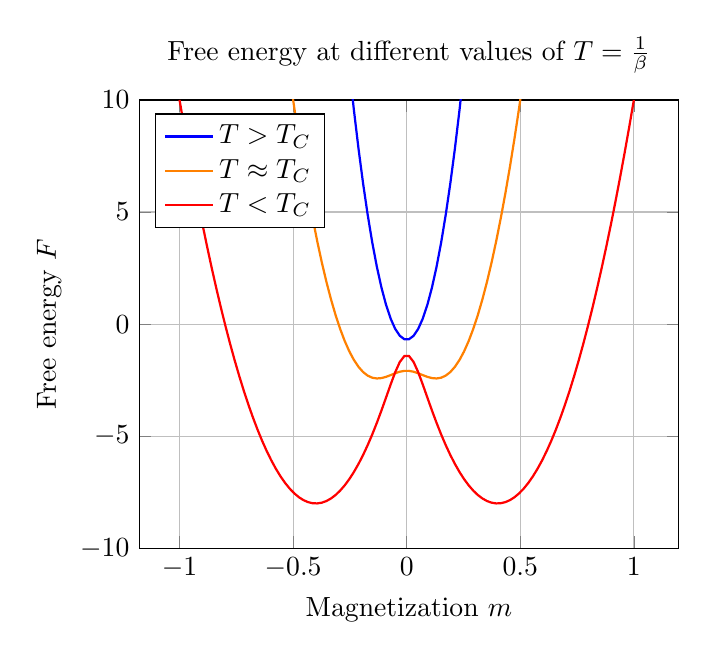
\begin{tikzpicture}
        \begin{axis}[
            ylabel=Free energy $ F$,
            xlabel=Magnetization $m$,
            ymin=-10,
            ymax=10,
            legend pos=north west,
            grid=major,
            title={Free energy at different values of $T=\frac{1}{\beta}$}
        ]
        \addplot[domain=-1:1, samples=100, blue, thick] {x^2*200 - 1 * ln(2*cosh(x/2*10))};
        \addlegendentry{$T> T_C$}
        \addplot[domain=-1:1, samples=100, orange, thick] {x^2*100 - 3 * ln(2*cosh(x*10))};
        \addlegendentry{$T \approx T_C$}
        \addplot[domain=-1:1, samples=100, red, thick] {x^2/2*100 - 2 * ln(2*cosh(x*20))};
        \addlegendentry{$T < T_C$}
        \end{axis}
        \end{tikzpicture}
    \label{Fig:free energy}
    \caption{Free energy of the system at different temperatures with a zero external field: here it is shown how $F$ goes from having a minimum in $m=0$ to having two distinct minima for $m\neq0$.}
\end{figure}
Known this, we can study these minima and so determine the magnetization of the system
\begin{equation}
    0=\frac{\partial F_{MS}}{\partial m}=Jz\{m-\tanh[\beta(Jmz+H)]\}, \quad \Rightarrow\quad m=\tanh[\beta(Jmz+H)],\label{mean_field_magnetization_equation}
\end{equation}
which is the solution of this transcendental equation. Unfortunately, being transcendental, this equation cannot be exactly solved, but we can determine when we transition from the single solution (the previous minimum in $m=0$) to multiple solutions (the two minima in $m=\pm1$ for example). Examining the graph (Fig. \ref{Fig:Soluzione m}) of the two functions equated by \eqref{mean_field_magnetization_equation} we can observe that, assuming no external field:
\begin{figure}[h]
    \centering
    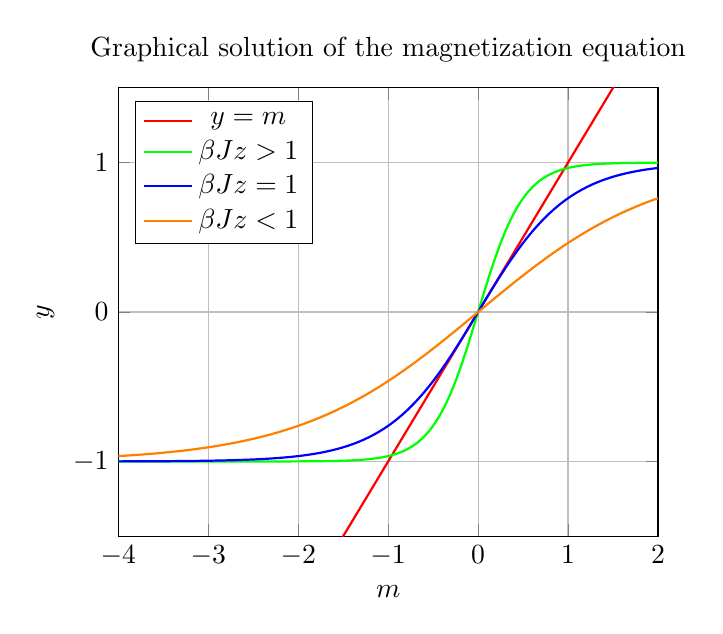
\begin{tikzpicture}
        \begin{axis}[
            xlabel=$m$,
            ylabel=$y$,
            ymin=-1.5,
            ymax=1.5,
            xmin=-4,
            xmax=2,
            legend pos=north west,
            grid=major,
            title={Graphical solution of the magnetization equation}
        ]
        \addplot[domain=-4:2, samples=2, red, thick] {x};
        \addlegendentry{$y = m$}
        \addplot[domain=-4:2, samples=100, green, thick] {tanh(2*x)};
        \addlegendentry{$\beta Jz>1$}
        \addplot[domain=-4:2, samples=100, blue, thick] {tanh(x)};
        \addlegendentry{$\beta Jz =1$}
        \addplot[domain=-4:2, samples=100, orange, thick] {tanh(0.5*x)};
        \addlegendentry{$\beta Jz<1$}
        \end{axis}
        \end{tikzpicture}
    \label{Fig:Soluzione m}
    \caption{Resolution of the implicit equation defining the magnetization for 3 different temperatures.}
\end{figure}
\begin{itemize}
    \item if $\frac{\partial}{\partial m}\tanh(\beta Jmz)\big|_{m=0}=\beta Jz\leq1$ then we have only one point of intersection in $m=0$;
    \item if $\frac{\partial}{\partial m}\tanh(\beta Jmz)\big|_{m=0}=\beta Jz>1$ then we have 3 intersections between the two functions.
\end{itemize}
This shows us that there is a temperature, that we call \textbf{critical temperature} $T_c=Jz$, before which the magnetization is exactly zero, and then it transitions to being non-zero, since a further inspection of the above stationary points will show that for $T>T_c$ the point $m=0$ becomes a maximum.

Even though we showed that the system spontaneously transitions between a magnetized state to a zero magnetization state, we haven't showed that this is a phase transition, we will now look for discontinuity in the thermodynamic variables. Consider the magnetic susceptibility
\begin{equation*}
    \chi=\frac{\partial m}{\partial H}=\frac{\partial }{\partial H}\tanh(\beta(Jzm+H))=\beta\frac{1+Jz\frac{\partial m}{\partial H}}{\cosh^2[\beta(Jzm+H)]},
\end{equation*}
once solved this equation can be evaluated at the critical temperature in absence of external fields to get
\begin{equation}
    \chi(H=0,T=JZ)=\frac{\beta}{\cosh^2(\beta(Jzm+H))-JZ\beta}\bigg|_{H=0,T=JZ}\rightarrow\infty.
\end{equation}
We should also mention that the specific heat at constant volume diverges at the critical temperature, however the mean field approximation cannot show this discontinuity.
\subsubsection{Spontaneous symmetry breaking}
We should highlight a peculiar propriety of the Ising model. Notice that the Hamiltonian \eqref{Ising_Hamiltonian}, in absence of the external field $H$, is invariant under the discrete symmetry $\mathbb{Z}_2$, defined by $\sigma_i\rightarrow\sigma_i'=-\sigma_i$. Note that the interaction with the external magnetic field explicitly breaks this symmetry: we could interpret $\mathbb{Z}_2$ as a consequence of isotropy of space, in this way the external field defines a preferred direction breaking the isotropy of space.

From this symmetry, we could argue that at equilibrium we should be in a $\mathbb{Z}_2$ invariant state, a state for which $m=0$. As we saw this is not true at every temperature: above the critical temperature the magnetization is zero, and thus we respect $\mathbb{Z}_2$ symmetry, while below the critical temperature the magnetization is non-zero, breaking the symmetry. Note that the Hamiltonian possesses the $\mathbb{Z}_2$ symmetry in both cases, therefore there is none explicit breaking of the symmetry, on the contrary with what happened with the external field. Even the mean field interaction term of \eqref{mean_field_hamiltonian} does not break the symmetry, since if $\sigma_i\rightarrow\sigma_i'=-\sigma_i$ also $m\rightarrow m'=-m$ (in the Hamiltonian appears their product). In this case we have a \textbf{spontaneous breaking of the symmetry}.

What actually happens here is that the "\emph{ground state}" breaks the symmetry, since as we saw a single minimum splits into two different minima, then the system could hypothetically remain in a stationary state which preserve the symmetry (in this case $m=0$) but that would be an unstable state. At this point thermal fluctuations are enough to move the system to a minimum breaking the symmetry.

This kind of behavior, not only is interesting to be studied per se, but it revealed to be key into the development of many deep mechanisms of nature, first over all the Higgs mechanism that gives mass for example to gauge bosons in the standard model. 

\subsubsection{Exact solutions}
We employed the mean field approximation just to illustrate the general behavior that we should expect from the system, however if we want to study this system some exact results should be used too. 

Mean field approximation fails for a lattice of dimension 1, since it would predict a $T_c=2J$ while the exact solution predicts that there is no spontaneous symmetry breaking in this case. For higher dimension than 4 the approximation become suitable while at lower the exact results can differ, as happens for dimension 1. In dimension 2, some non-trivial exact solutions can be found: we present the exact critical temperature for some simple topology of the lattice, these results can be found in \cite{ExactIsing}:
\begin{align}
    &\text{Square lattice: } &T_c^S&=\frac{2}{\log(1+\sqrt{2})}J &\simeq 2.26929 J,&&\\
    &\text{Triangular lattice: } &T_c^T&=\frac{2}{\log(\sqrt{3})}J &\simeq 3.64096 J,&&\\
    &\text{Hexagonal lattice: } &T_c^H&=\frac{2}{\log(2+\sqrt{3})}J &\simeq 1.51865 J.&&
\end{align}
These results can be compared to the mean field ones: $T_c^{S}=4J,\ T_c^{T}=6J$ and $T_c^H=3J$. In this way we can see that mean field approximations should be considered as an estimate of an upper bound of the critical temperatures.

\subsection{Networks and their proprieties}
A network, mathematically speaking, is defined as a pair of sets $(V,\ E)$, where elements of $V$ are called \textbf{vertices} and $E$ is a set of pairs of vertices, called \textbf{edges}. We also call the vertices \textbf{nodes} and the edges \textbf{links}. With this structure we can describe a set of points ($V$), that can represent some data, and how they are connected each other, through the links.
\begin{figure}[h]
    \centering
    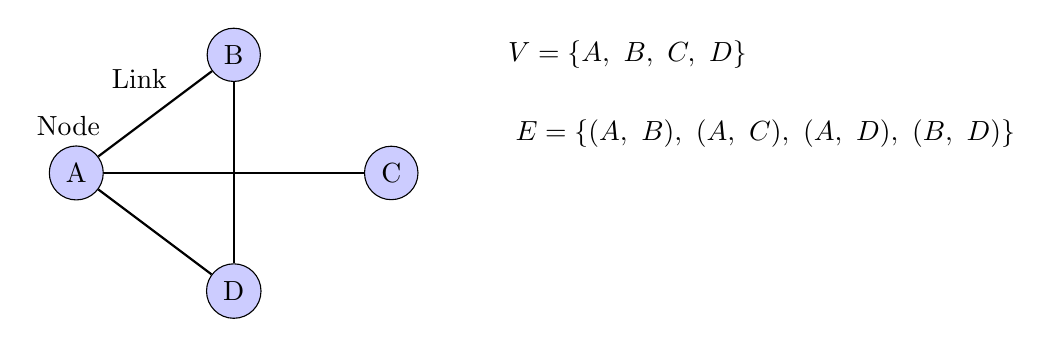
\begin{tikzpicture}
        \node[circle, draw, fill=blue!20] (A) at (0,0) {A};
        \node[circle, draw, fill=blue!20] (B) at (2,1.5) {B};
        \node[circle, draw, fill=blue!20] (C) at (4,0) {C};
        \node[circle, draw, fill=blue!20] (D) at (2,-1.5) {D};
        \node at (-0.1,.6) {Node};
        
        \draw[ thick] (A) -- (B);
        \draw[ thick] (A) -- (C);
        \draw[ thick] (A) -- (D);
        \draw[ thick] (B) -- (D);
        \node at (.8,1.2)  {Link};

        \node at (7,1.5)  {$V=\{A,\ B,\ C,\ D\}$};
        \node at (8.75,0.5)  {$E=\{(A,\ B),\ (A,\ C),\ (A,\ D),\ (B,\ D)\}$};
    \end{tikzpicture}
    \label{Fig:General Network}
    \caption{Pictorial representation of a network: each point is a node and each line connecting nodes is a link.}
\end{figure}  

Network theory can easily be applied to the Ising model in order to describe the lattice structure: each node can represent an atom and each link the possible interactions between neighbors. In this way we also manage to use more general structures, other than square, triangular and hexagonal lattices, that can be then studied numerically. Furthermore, this theory allows us to study the proprieties of a network by measuring some quantities that can be then used to analyze its structure.
\subsubsection{Topologies of a network}
As we already said, using networks to describe the lattice allows us to easily study, by numerical methods, different types of topologies in different dimensions: starting from $2D$ lattices with different structures, square, triangular, hexagonal lattices, to $3D$ lattices to Erdős–Rényi graphs and so on. Let's spend some time analyzing the graph that we used.

Lattices are regular networks that periodically repeat a basic structure: square lattices are made by the repetition of 4 nodes connected together into a square, triangular by 3 nodes to form a triangle and lastly hexagonal are made by groups of 6 nodes forming hexagons. These structures can also be created in 3 dimensions or higher.

Herdos Renyl graphs are networks made up by a fixed number of nodes $N$ and are characterized by a probability $p$: this is the probability that a pair of nodes is connected by a link. In this way the number of links connected to a node (degree of the node) follows the binomial distribution.

Lastly, we used some more specific networks: we call \emph{broken lattices} lattices from which we removed a fraction of vertices (and their edges), and \emph{more than nearest neighbors} lattices in which we connected each node to the neighbors of its neighbors.


\subsubsection{Measuring proprieties of networks}
To end our introduction on networks, we will now illustrate the main quantities that we aim to measure in our simulation of the Ising model.
\begin{itemize}
    \item \textbf{Network density}: this parameter measure how many links are present in a network compared to the maximum number of links possible given the nodes, it is defined as:
    \begin{equation}
        d=\frac{2m}{n(n-1)},\label{density}
    \end{equation}
    where $m$ is the number of edges and $n$ the number of nodes, $\frac{n(n-1)}{2}$ is the maximum number of edges given $n$ nodes.
    \item \textbf{Diameter}: this measures the minimum number of links connecting the two farthest nodes of a connected graph (if every point can be reached moving along the graph starting from every other point), it is defined as:
    \begin{equation}
        D=\max_{i,j} D_{i,j},\label{diameter}
    \end{equation}
    where $D_{ij}$ is the geodesic distance between node $i$ and $j$, which is the number of links of the shortest path connecting $i$ to $j$.
    \item \textbf{Betweenness centrality}: for every node we can measure how the network changes removing 1 node, this is done by this quantity defined by:
    \begin{equation}
        \label{Betweenness centrality}
        B_i=\sum_{j,k\neq i}\frac{N_{jik}}{N_{jk}},
    \end{equation}
    where $N_{jik}$ is the number of the shortest path starting form the node $j$, passing for the node $i$ and ending in the node $k$ and $N_{jk}$ are the shortest path from the node $j$ to node $k$, in this way we measure the fraction of the shortest paths that would be broken by removing the $i$-th node.
    \item \textbf{Node connectivity}: this quantifies the minimum number of nodes needed to be removed in order to disconnect the graph or make it trivial.
\end{itemize}
Note that all the networks described in the previous section have precise proprieties, therefore we won't measure these quantities for the lattice networks, but we will study the networks emerging from the Ising dynamic.

Discussing these proprieties we introduced the concept of a connected graph, for which every pair of point can be connected moving along the network, however this implies that there can be also network that are disconnected. This kind of networks are composed by at least two connected subnetworks: it can be interesting to study the proprieties of these connected components, for this reason we use the \textbf{number of connected components} and the \textbf{giant component}, which is the largest connected component. The giant component can then be used to study the behavior of those quantities, as the betweenness centrality, that cannot be defined on disconnected networks. 

\section{Implementation of the model}
To simulate the Ising model we generated a network using the Phyton library \textbf{Networkx}, then we assigned a random spin, $\pm1$, to each node. Given an initial temperature we thermalized the system using the Metropolis-Hastings algorithm, that we will describe in the next sections. When thermalization is reached we started measuring the quantities we are interested in. This procedure is repeated for a set of different temperatures to obtain the thermodynamic variables and the network measures as functions of the temperature.
All the code that we used is available in our repo: \url{https://github.com/MorelliLuca/Complex_Network_Ising_Model.git}.
\subsection{The Metropolis-Hastings algorithm}
To obtain an equilibrium microstate of a system, monte carlo methods can be used, for our purpose the \textbf{Metropolis-Hastings algorithm} can mimic the thermal fluctuations that are generated by a thermal bath in canonical ensemble.

The main idea behind this algorithm is that, if we have two different states of our system, say $A$ and $B$, and we know the probability of finding the system in each state, say $P(A)$ and $P(B)$, we can connect the two probabilities by the probability of transitioning $A\rightarrow B,\ P(A\rightarrow B)$
\begin{equation*}
    P(B)=P(A\rightarrow B)P(A)\qquad \Leftrightarrow\qquad P(A\rightarrow B)=\frac{P(B)}{P(A)}.
\end{equation*}
In the canonical ensemble the probability of observing the microstate with energy $E_A$ is given by the Boltzmann exponential divided by the canonical partition function, in this way we can easily determine the transition probability between two states of different energies
\begin{equation*}
    P(E_A)=\frac{e^{-\beta E_A}}{Z}\qquad \Rightarrow\qquad P(E_A\rightarrow E_B)=e^{-\beta(E_B-E_A)}.
\end{equation*} 
Note that when $E_B-E_A<0$, the new microstate has a grater energy than the starting one, the probability that the transition occurs is grater then one, in this case we just assume that the probability is one. This could seem a bold assumption, but actually it follows from the idea that equilibrium is reached at minimum of the (free) energy. Our criterion thus become
\begin{equation}
    \label{MHCriterion}
    P(E_A\rightarrow E_B)=\begin{cases}
        1\qquad\qquad\quad\ \  \text{if}\ E_B<E_A\\
        e^{-\beta(E_B-E_A)}\quad \text{if}\ E_B>E_A
    \end{cases}.
\end{equation}
Now, the Metropolis-Hastings algorithm explores the phase space of our system by flipping one random spin at the time, then for each flip we evaluate the variation of the energy, and we decide whether the flip occurs using the criterion \eqref{MHCriterion}. Iterating this procedure, as we already said, we mimic the thermal fluctuation induced by a bath of a given temperature $\beta$, after a big number of iterations the system reaches equilibrium with the bath. The number of iteration needed to reach equilibrium is called \emph{thermalization time} and will vary with the dimension of the phase space that the system has to explore.

A useful feature of this algorithm is that, once reached equilibrium, the system will remain at equilibrium exploring just a neighborhood of the equilibrium microstates. In this way, by continuing the iteration at equilibrium for a sufficient number of steps, in order to suppress the correlations with the first microstate that we found at equilibrium, we can obtain other microstates at equilibrium. These can be then used to measure thermal averages over a fictitious ensemble. The main advantage of this procedure is that the thermalization time is usually grater then the number of steps needed to suppress the correlation between microstates, in this way we can obtain an ensemble in more efficient and faster way than restarting again the whole procedure.

For our simulation the algorithm has been repeated for each temperature, but, since the thermalization time grows with the number of atoms and in theory we would like to reach the thermodynamic limit $N\rightarrow\infty$, we used a trick. If the difference between successive temperatures is small, the "distance" in phase space between the old equilibrium states and the new ones should be small too. For this reason, after the first run at the first temperature, we make evolve the system from the last microstate found to the new temperature, for a number of iteration sufficient to lose correlations between old states and the new ones. In this way the full thermalization has to occur just one time and then each thermalization between each successive temperature is greatly reduced.

\subsection{Measure procedure}
As already mentioned, the Metropolis-Hasings algorithm allows us to efficiently create a canonical ensemble of our system at each temperature. To obtain $N$ samples every $\Delta$ steps (needed to remove correlations) we measured the desired quantities only in the $N\cdot \Delta$ last iterations of the evolution process between successive temperatures, assuming that when we start measuring the system has already reached equilibrium. Then, for each temperature, we averaged over those measures.
\subsubsection{Thermodynamic measures}
Thermodynamic variables are often related one to the other, for this reason some of them cannot be directly measured, but they must be obtained from some that can be measured directly.

We now describe the procedure used to obtain these last ones.
\begin{itemize}
    \item The \textbf{energy} can be evaluated at each step from the Hamiltonian \eqref{Ising_Hamiltonian} (remember that we need to know it for the Metropolis-Hasings algorithm) however this wouldn't be very efficient, since we should go through the whole network and for each atom through its neighbors: for this reason we evaluated it just one time in the beginning, then at each step we calculated the energy contribution of just the flipped spin, since the spin can either be $+1$ or $-1$ the variation of the total energy is twice the energy of the flipped spin.
    \item The \textbf{magnetization} could be evaluated averaging the spins of all the atoms, however again this process can be optimized since the change of magnetization due to a spin flip is just twice its new spin over the number of atoms, for this reason we calculated the full magnetization just at the beginning and the for each step we update it.
    \item The \textbf{entropy} is easily obtained as a function of the magnetization using the micro-
    canonical formula and the Stirling approximation 
    \begin{align*}
        S=\log\omega=\log\frac{N!}{N_+!N_-!}&\simeq N\log N-N-(N_+\log N_+-N_++N_-\log N_--N_-)\\
        &=-N\bigg(\frac{1+m}{2}\log{\frac{1+m}{2}}+\frac{1-m}{2}\log{\frac{1-m}{2}}\bigg).
    \end{align*} 
    \item The \textbf{free energy} is evaluated at each step from its definition $F=E-TS$. 
\end{itemize}
From these we can obtain the \textbf{heat capacity} and the \textbf{magnetization}. Consider the so-called generating function
\begin{equation}
    W(\beta, H)=\log Z_N(\beta, H)=-\beta F(\beta, H),
\end{equation}
recalling the discussion of section 1.1, we can use this function to obtain the above quantities:
\begin{align*}
    NC_V&=\frac{\partial E}{\partial T}= \beta^2\frac{\partial^2\log Z_N}{\partial\beta^2} =\beta^2\frac{\partial^2 W}{\partial\beta^2},\\\quad N\chi&=N\frac{\partial m}{\partial H}=N\frac{\partial}{\partial H}\frac{\left\langle\sigma_i \right\rangle }{N}=\beta\frac{\partial^2 \log Z_N}{\partial H^2}=\beta\frac{\partial^2 W}{\partial H^2}.
\end{align*}
We can calculate the last derivatives of each of the above lines to get 
\begin{align*}
    \frac{\partial^2 W}{\partial\beta^2}&=\frac{\partial^2 \log Z_N}{\partial\beta^2}= \frac{\partial}{\partial\beta}\frac{1}{Z_N}\frac{\partial}{\partial\beta}\sum_{\{\sigma_i\}} \exp(-\beta\mathcal{H} )=-\frac{\partial }{\partial\beta}\frac{1}{Z_N}\sum_{\{\sigma_i\}}\mathcal{H} \exp(-\beta\mathcal{H} )
    \\&=\frac{\sum_{\{\sigma_i\}}\mathcal{H}^2 \exp(-\beta\mathcal{H} )}{Z_N}-\frac{[\sum_{\{\sigma_i\}}\mathcal{H} \exp(-\beta\mathcal{H} )]^2}{Z_N^2}=\left\langle E^2 \right\rangle-\left\langle E \right\rangle^2\\
    \frac{\partial^2 W}{\partial H^2}&=\frac{\partial^2 \log Z_N}{\partial H^2}=\frac{\partial}{\partial H}\frac{1}{Z_N}\frac{\partial}{\partial H}\sum_{\{\sigma_i\}} \exp(-\beta\mathcal{H} )=\frac{\partial}{\partial H}\frac{\beta}{Z_N}\sum_{\{\sigma_i\}}\sum_{i=1}^N \sigma_i \exp(-\beta\mathcal{H} )
    \\&=\frac{\sum_{\{\sigma_i\}}(\sum_{i=0}^N\sigma_i)^2 \exp(-\beta\mathcal{H} )}{Z_N}-\frac{[\sum_{\{\sigma_i\}}\sum_{i=0}^N\sigma_i \exp(-\beta\mathcal{H} )]^2}{Z_N^2}=\left\langle m^2 \right\rangle-\left\langle m \right\rangle^2.
\end{align*}
Putting these results together we discover that the heat capacity and the susceptibility are a measure of the dispersion from the mean of, respectively, the energy and magnetization:
\begin{equation}
    C_V=\frac{\left\langle E^2 \right\rangle-\left\langle E \right\rangle^2}{NT^2},\qquad \chi=\frac{\left\langle m^2 \right\rangle-\left\langle m \right\rangle^2}{NT}.
\end{equation}
These two formulae give us a simple way to measure the heat capacity and the susceptibility, however these must be extracted from the ensemble measures (they need means in the first place) and therefore we haven't measured their average but one single value for each temperature.
\subsubsection{Graph measures}
All the network measures (the quantities of section 1.2.2) are obtained using the Networkx (for more informations \cite{Networkx}) features. For each one we evaluated the average as we have done with the thermodynamic variables.

For each iteration in which a measure occurred we separated the network in two, one containing only \emph{spin up} atoms, and another with only \emph{spin down}, preserving the links of the lattice that connected neighbor aligned spins. Then the measures was conducted on the two networks. As already explained, for some quantities we need connected networks, however this splitting procedure generates also disconnected graphs, for this reason some measures was restricted only on the giant component of each network. Lastly, we compared the results obtained from the spin up and spin down networks.
\section{Discussion of the results}
We conducted 2 main types of measurements: the first ones are intended to check whether our simulation is compatible with the theoretical predictions, then we started studying the network behavior. We will now discuss these results using different types of networks.
\subsection{Seeking the phase transition}
To understand if our simulations agree with the theoretical predictions, we compared the phase transition temperatures (measured) with the predicted one from theory. Since the measuring procedure for these quantities is not so computationally heavy, we let the simulation thermalize for longer times, taking more measures, and we also used bigger lattices.

We simulated, with $J=50$, a square lattice of 900 atoms, a triangular lattice of 496 atoms and a hexagonal lattice of 38 atoms. At each temperature we obtained an ensemble of 3000 systems, one every 100 steps. The agreement between the model and the simulation is appreciable from Figure \ref{Fig:Behaviour1}, \ref{Fig:Behaviour2} and \ref{Fig:Behaviour3}, which show the phase transition in the magnetization, the entropy, in the susceptibility and in the heat capacity.

\begin{figure}[!htb]
    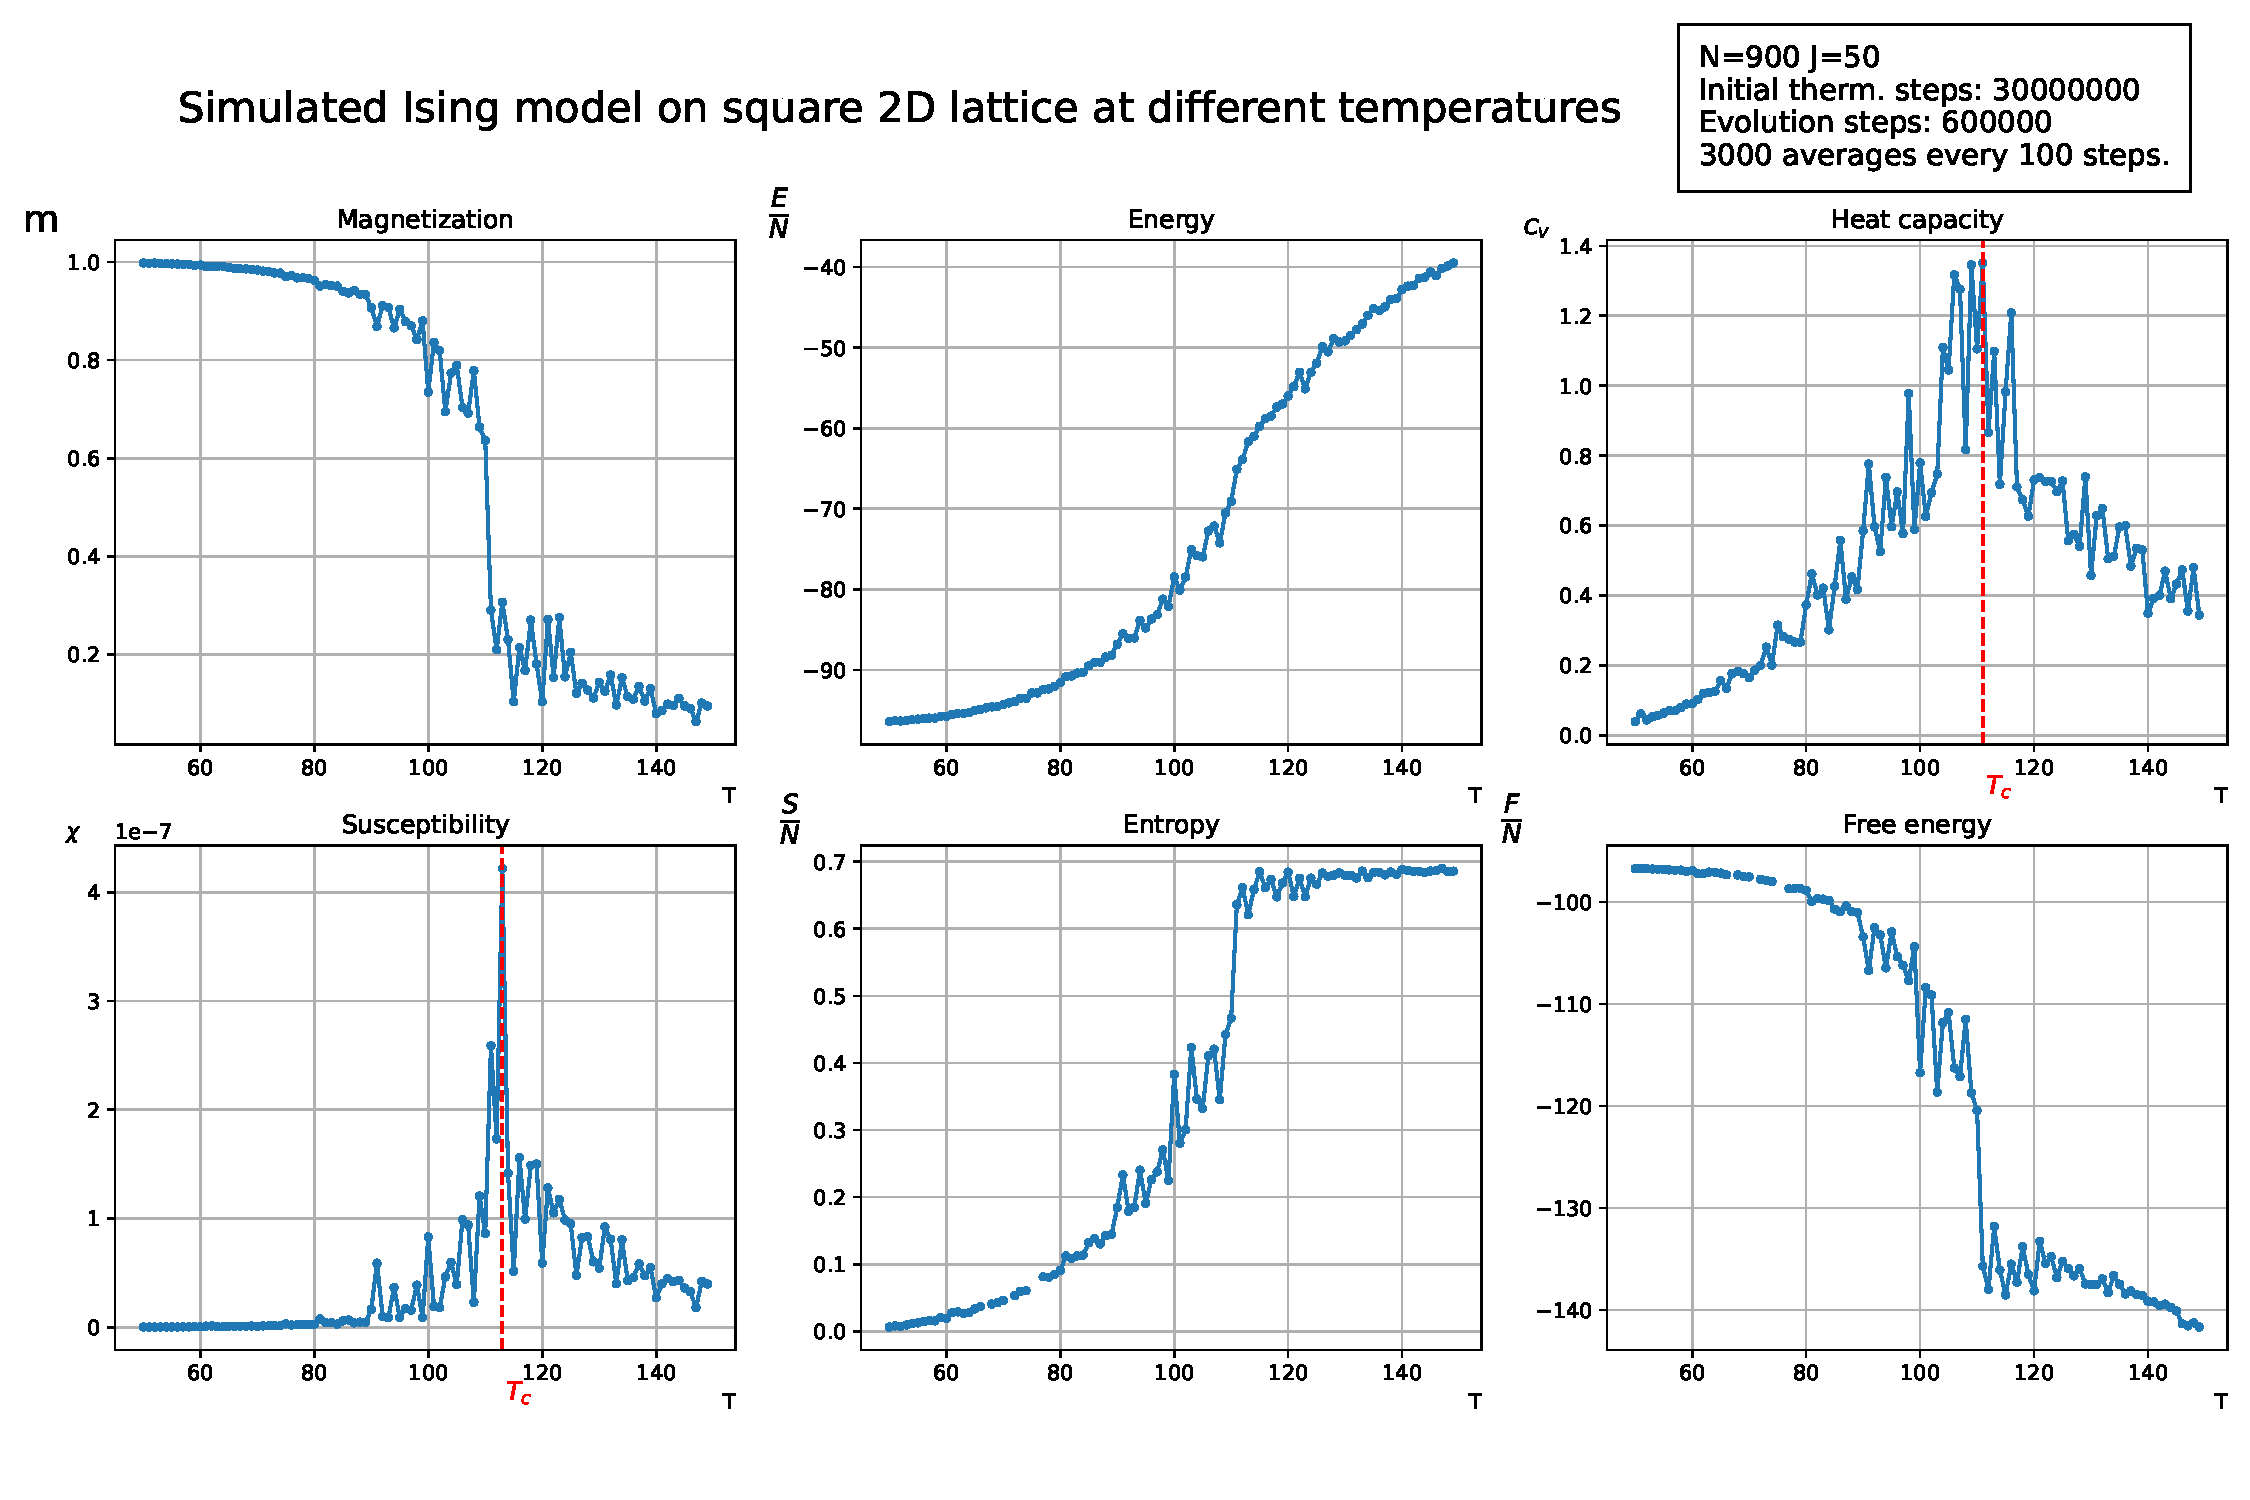
\includegraphics[width=\linewidth]{2d_square_thermal.pdf}
      \caption{Behavior of the square lattice at increasing temperatures. We highlighted with a dashed line the critical temperatures we measured.}\label{Fig:Behaviour1}
\end{figure}

\begin{figure}[!htb] 
    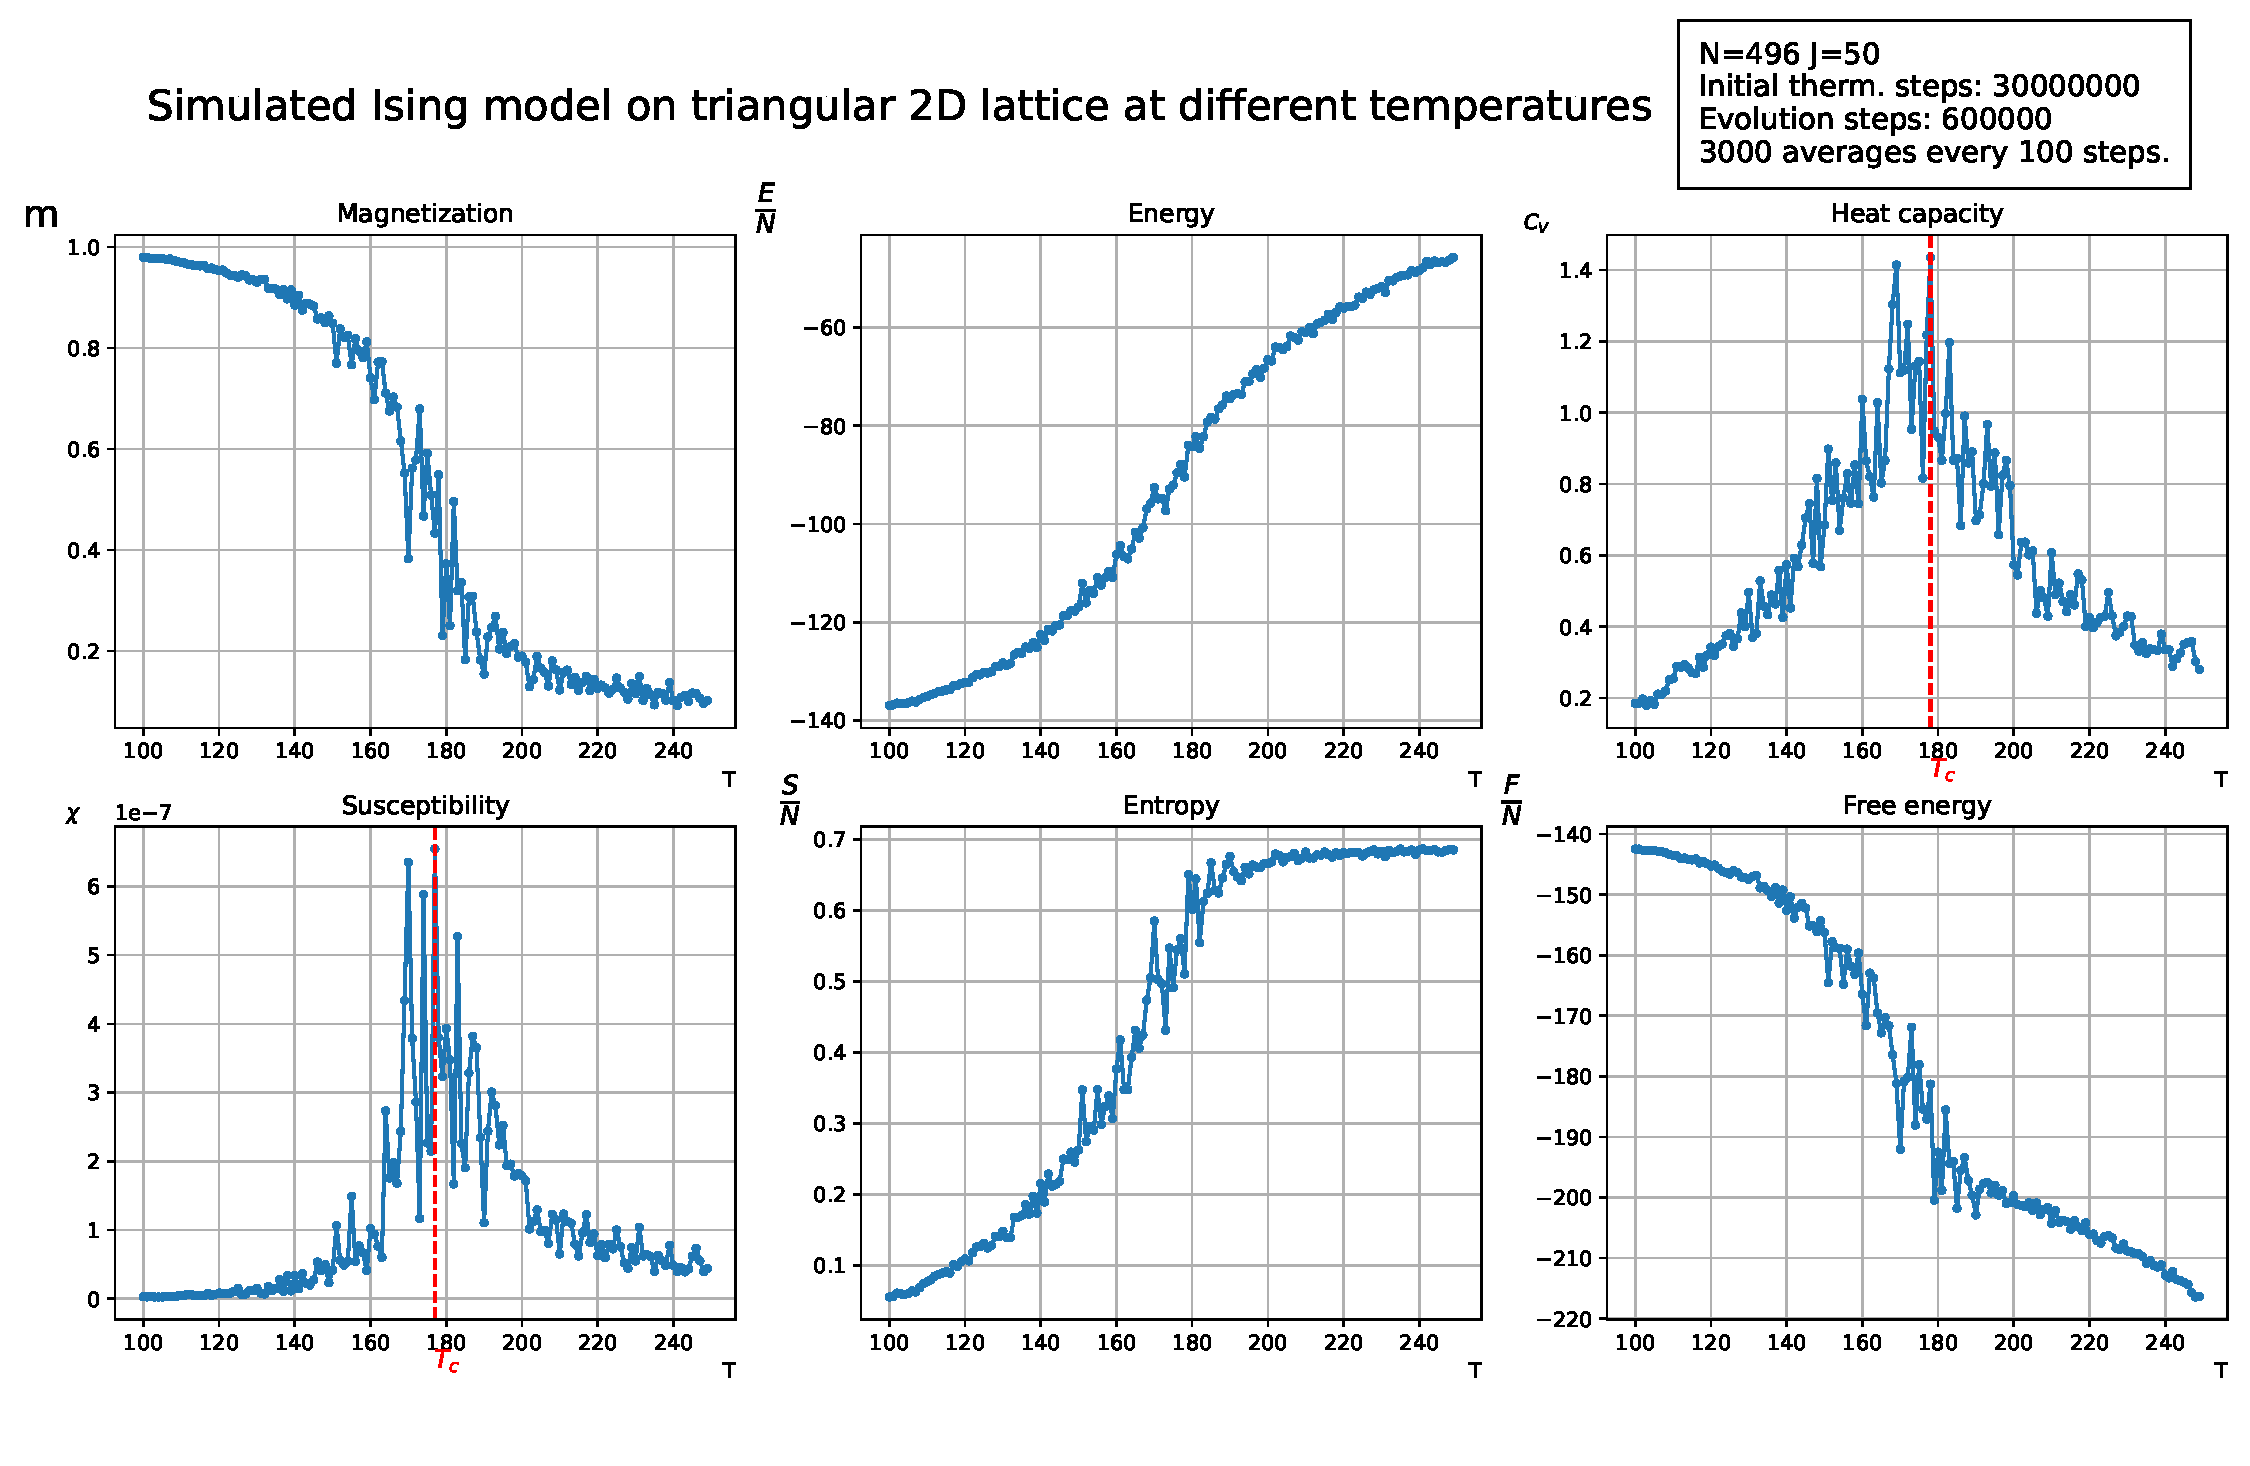
\includegraphics[width=\linewidth]{2d_triangular_thermal.pdf}
      \caption{Behavior of the triangular lattice at increasing temperatures. We highlighted with a dashed line the critical temperatures we measured.}\label{Fig:Behaviour2}
\end{figure}

\begin{figure}[!htb]
    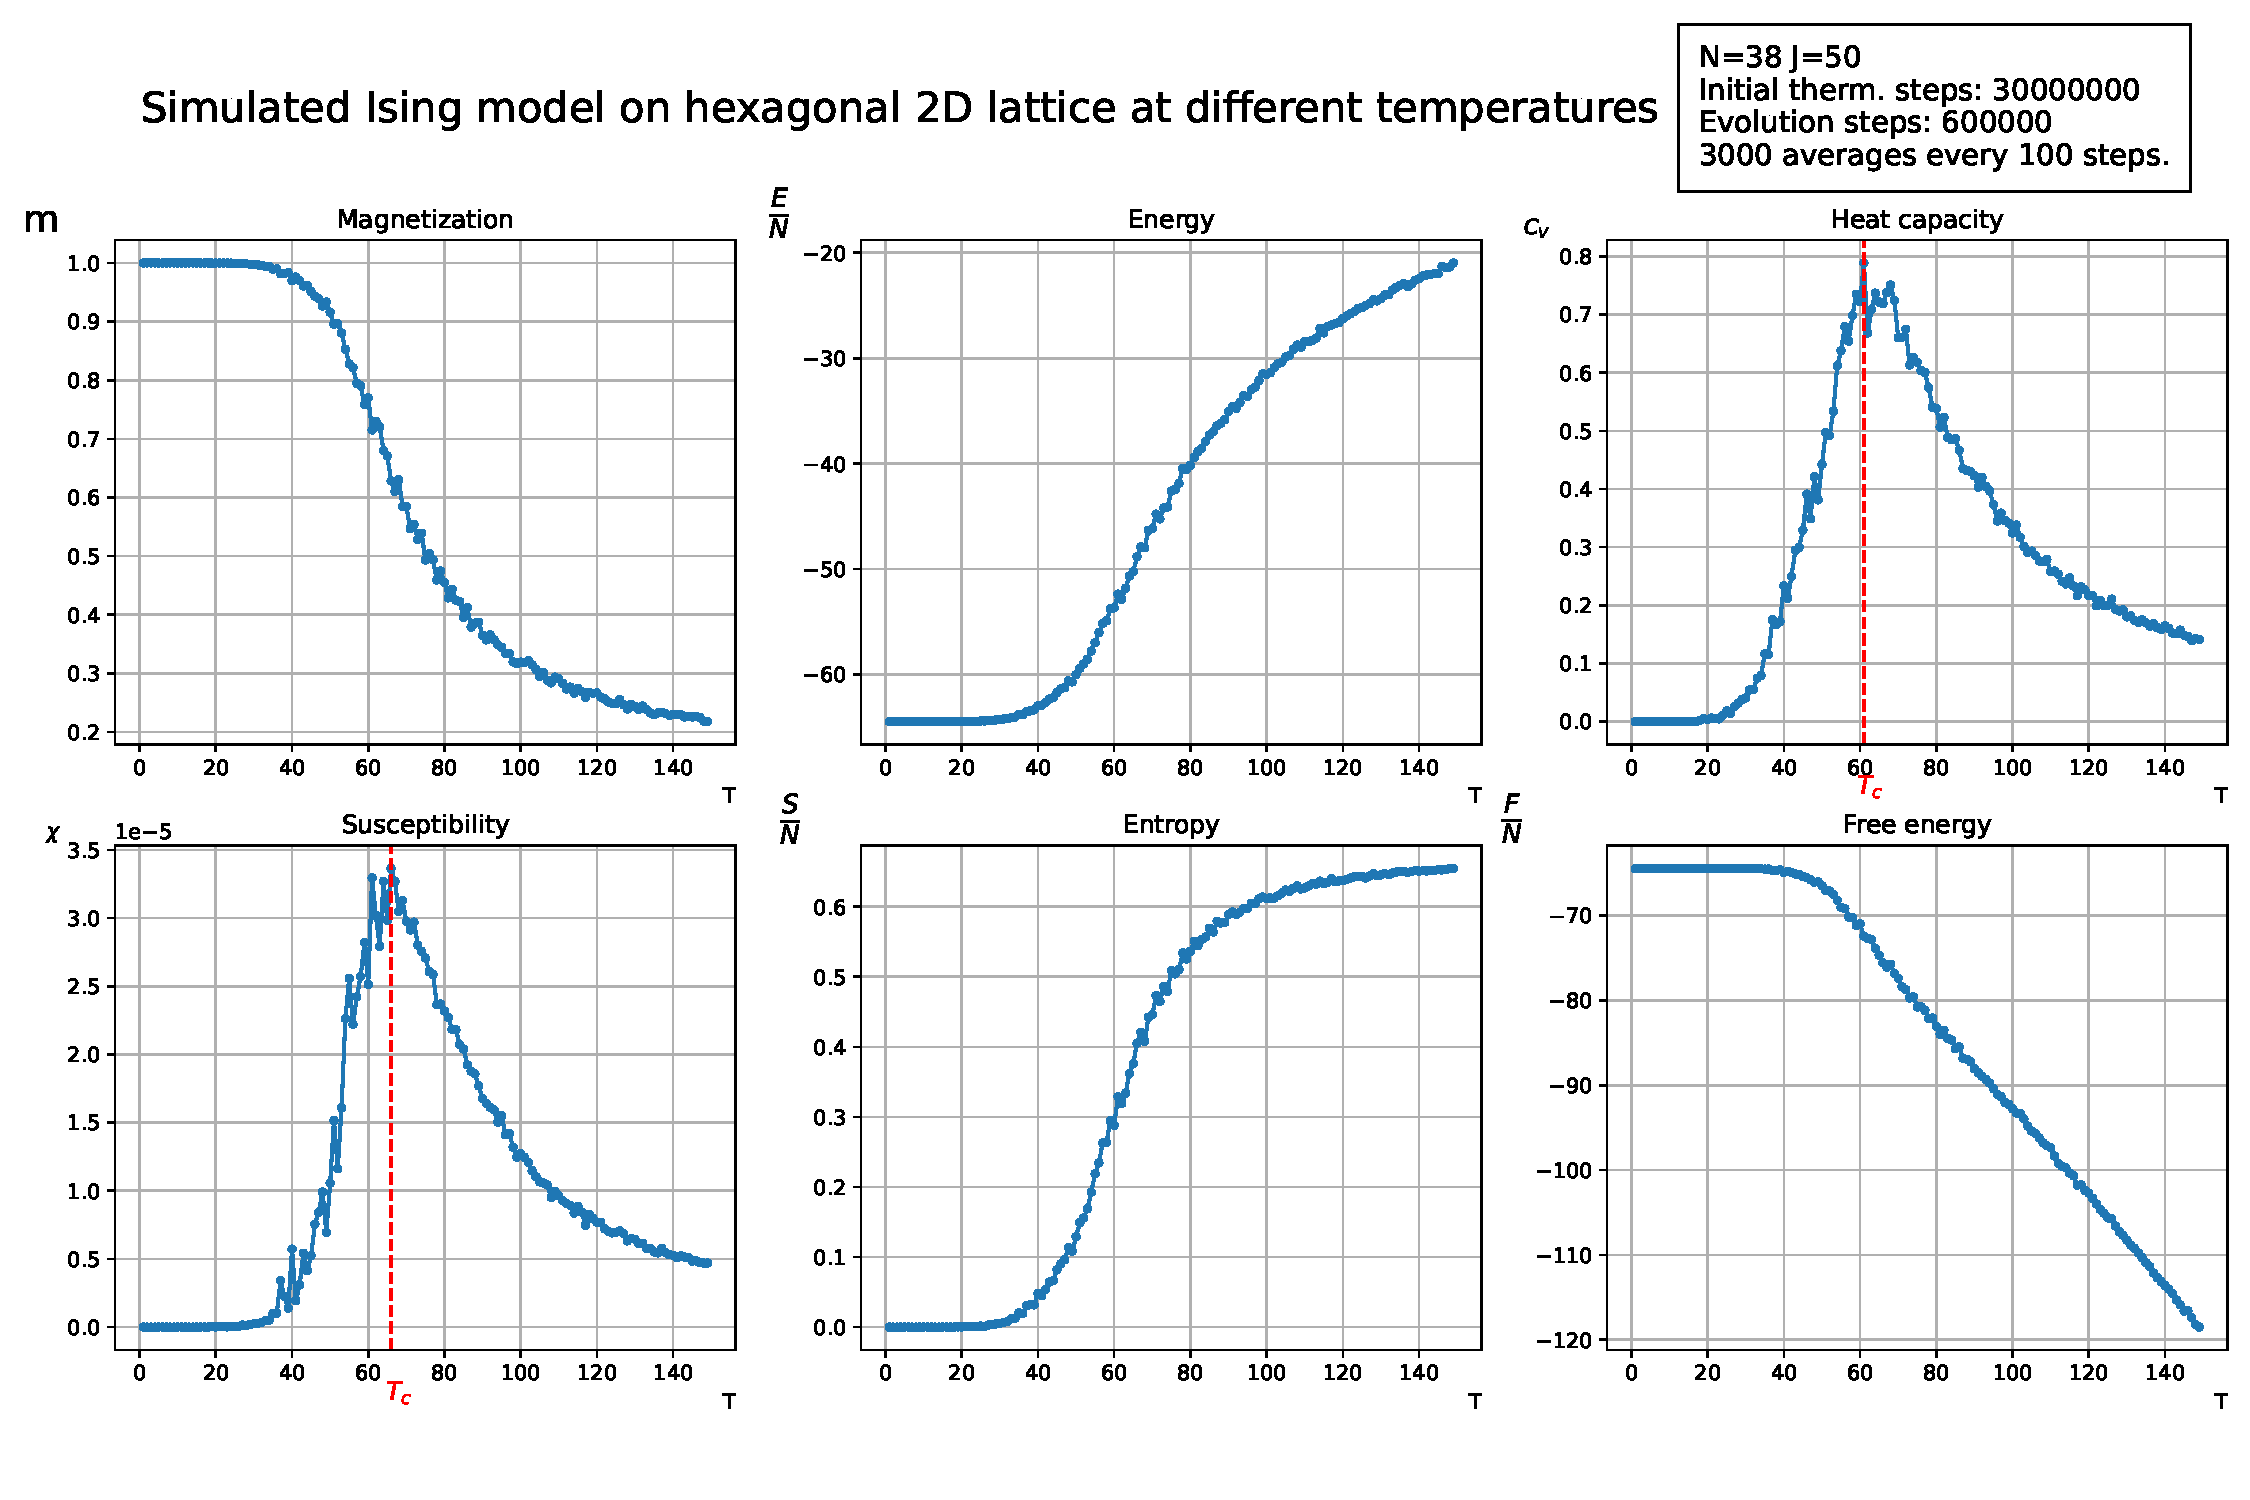
\includegraphics[width=\linewidth]{2d_hexagonal_thermal.pdf}
      \caption{Behavior of the hexagonal lattice at increasing temperatures. We highlighted with a dashed line the critical temperatures we measured.}\label{Fig:Behaviour3}
\end{figure}
We plotted the absolute value of the magnetization (to have a more readable plot), we can see that at low temperatures $m$ is close to 1, and then it quickly transitions to a zero magnetization around the critical temperature. Also the entropy, at the critical temperature, transitions from 0 to higher value, as we expected transitioning from ordered states to disordered ones. The heat capacity and the susceptibility also show the phase transition since, as expected, they have a peak around the critical temperatures. Lastly, the energy is constant at low temperatures and then, while transitioning, it increases, instead the free energy has the opposite behavior.

For each lattice we determined the phase transition temperature using the peak of the susceptibility and the heat capacity (which should diverge at $T=T_c$), then we compared the results with the theoretical predictions we previously discussed.
\begin{table}[!htbp]
    \centering
    \label{Tab:Check}
    \begin{tabular}{cccc}
        \toprule
        \multirow{2}{*}{Lattice} & \multicolumn{3}{c}{Critical temperature} \\
         \cmidrule(lr){2-4}
        & $C_V$ measure &  $\chi$ measure & Theoretical \\
        \midrule
        2D Square $30\times30$ & $1.11\times10^{2}$ & $1.13\times10^{2}$ & $1.134645\times10^{2}$ \\
        2D Triangular $30\times30$ & $1.78\times10^{2}$ & $1.77\times10^{2}$ & $1.82048\times10^{2}$ \\
        2D Hexagonal $4\times3$ & $6.1\times10^1$ & $6.6\times10^1$ & $7.5\times10^1$ \\
        \bottomrule
    \end{tabular}
    \caption{Comparison between measured and predicted critical temperatures for different lattices. Every measure was obtained from an ensemble of 3000 system every 100 steps at every $\Delta T=1$ with $J=50$.}
\end{table}

Table \ref{Tab:Check} shows that our model behaves in the predicted way since the measured critical temperatures are in agreement with the exact theoretical one. 

\subsection{The phase transition of the network}
We now want to study the behavior of the network itself as the temperature varies. As we already mentioned, we divided the network into the spin up and spin down networks to study them separately. In this way, when studying how these networks are connected (connected components, connectivity, and so on) we are studying how neighbors aligned atoms group together creating domains. Since the network measures are computationally heavy, we reduced the number of atoms and also the number of points that we measured: the next graphs will show measures repeated every $\Delta T=5$. Let's first analyze the simplest structure, the square lattice.

The first thing that we note in Figure \ref{Fig:squareNetworkmeasure} is that these graphs show really well the spontaneous symmetry breaking behavior, that otherwise only the non-zero magnetization would signal. Indeed, we can see that spin up and spin down networks behave in totally different ways at low temperature: initially all the spins all aligned, and thus they form 1 single connected component. As the temperature raises it starts to appear a second connected component of a few anti-aligned spins until, approaching the critical temperature, we start to get more  connected components and both networks break into smaller components. After the critical temperature the broken symmetry is restored and both networks behave in the same way: the number of components keeps to increase with the temperature while the size of the giant components asymptotically reaches 20 nodes. This shows that at high temperature aligned atoms still form two big connected networks containing almost half of the atoms each (one is spin up while the other spin down) with a few satellites small groups of atoms. However, the betweenness centrality, the diameter of the giant components and the average node connectivity of the giant components show that at higher temperatures the networks become less connected. The raise of the betweenness centrality means that the number of the shortest path that could be broken by removing 1 node increases. This is even better shown by the node connectivity: approaching 1 it signals that removing 1 single node is enough to disconnect the giant components. Lastly, the diameter shows that, even though the giant components are not chains, their structure is close to it: before the critical temperature we observe a single giant component with 50 atoms but with a small diameter of just 7 links, instead after the critical temperature each giant component becomes of around 20 atoms but with a higher diameter of almost 10 links. Lastly, we can observe that the density of links (the percentage of links of each network that exist over the possible ones) has a spike around the critical temperature.

\begin{figure}[!htb]
  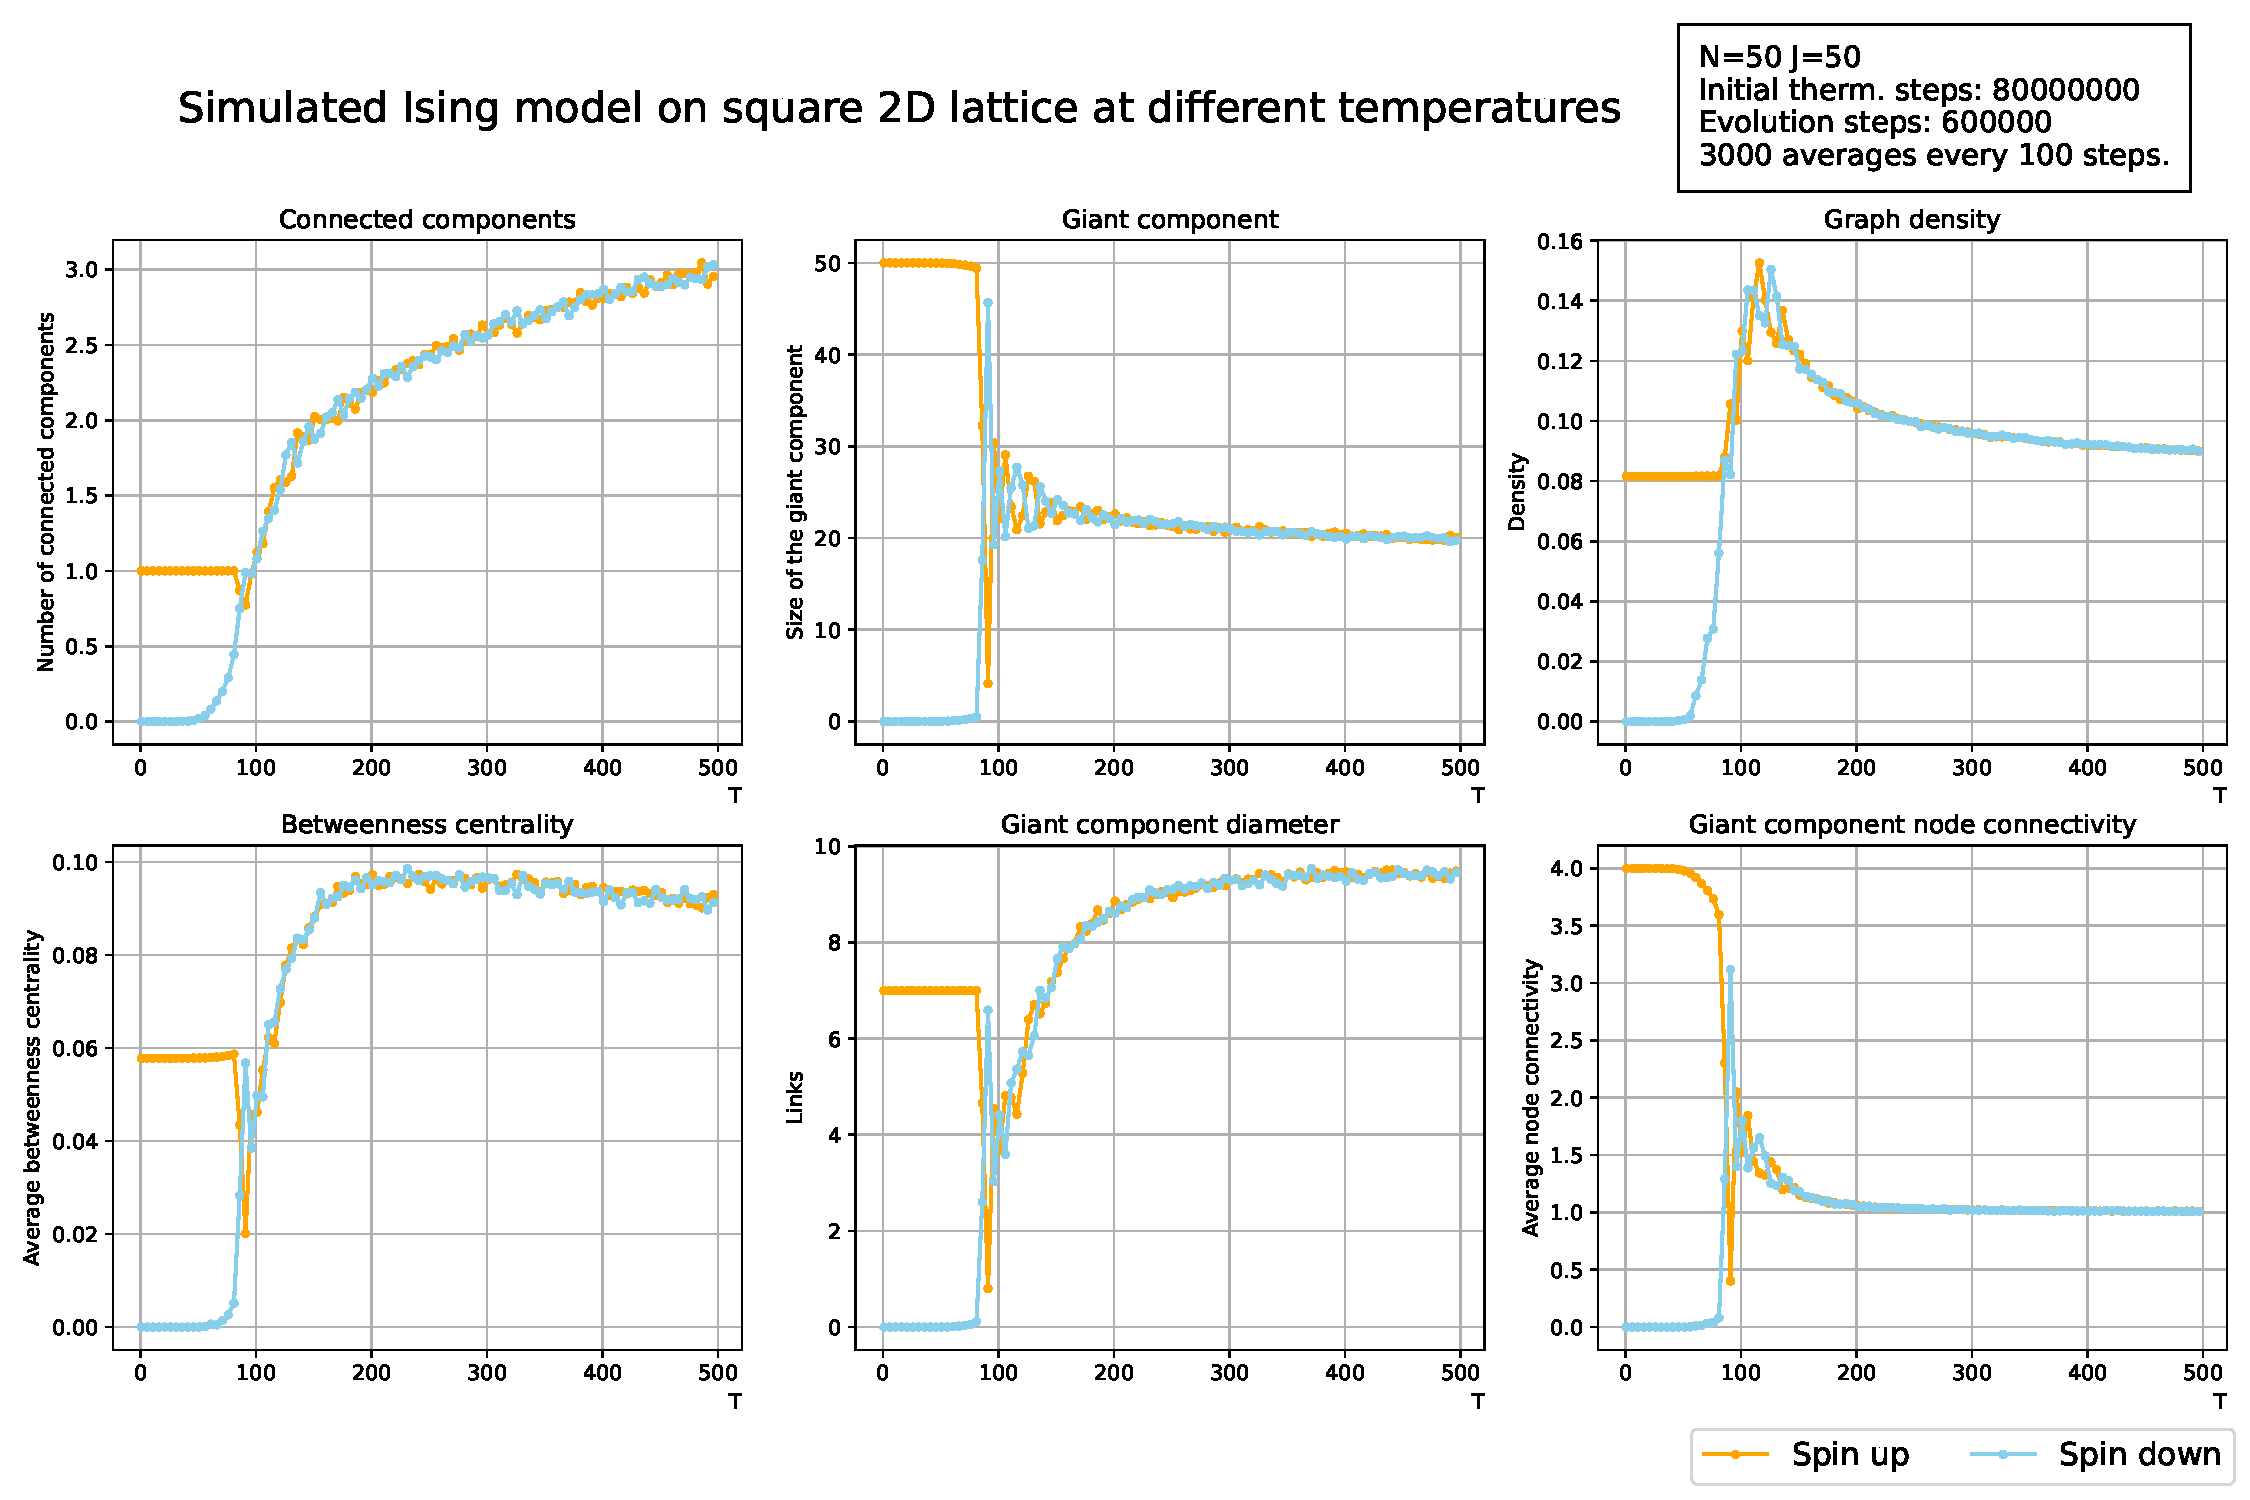
\includegraphics[width=\linewidth]{Network meausres/Square_Network.pdf}
    \caption{Behavior of the network proprieties of the square lattice at increasing temperatures. The orange line is the spin up network while the blue is the spin down one.}
    \label{Fig:squareNetworkmeasure}
\end{figure}

\begin{figure}[!htb]
  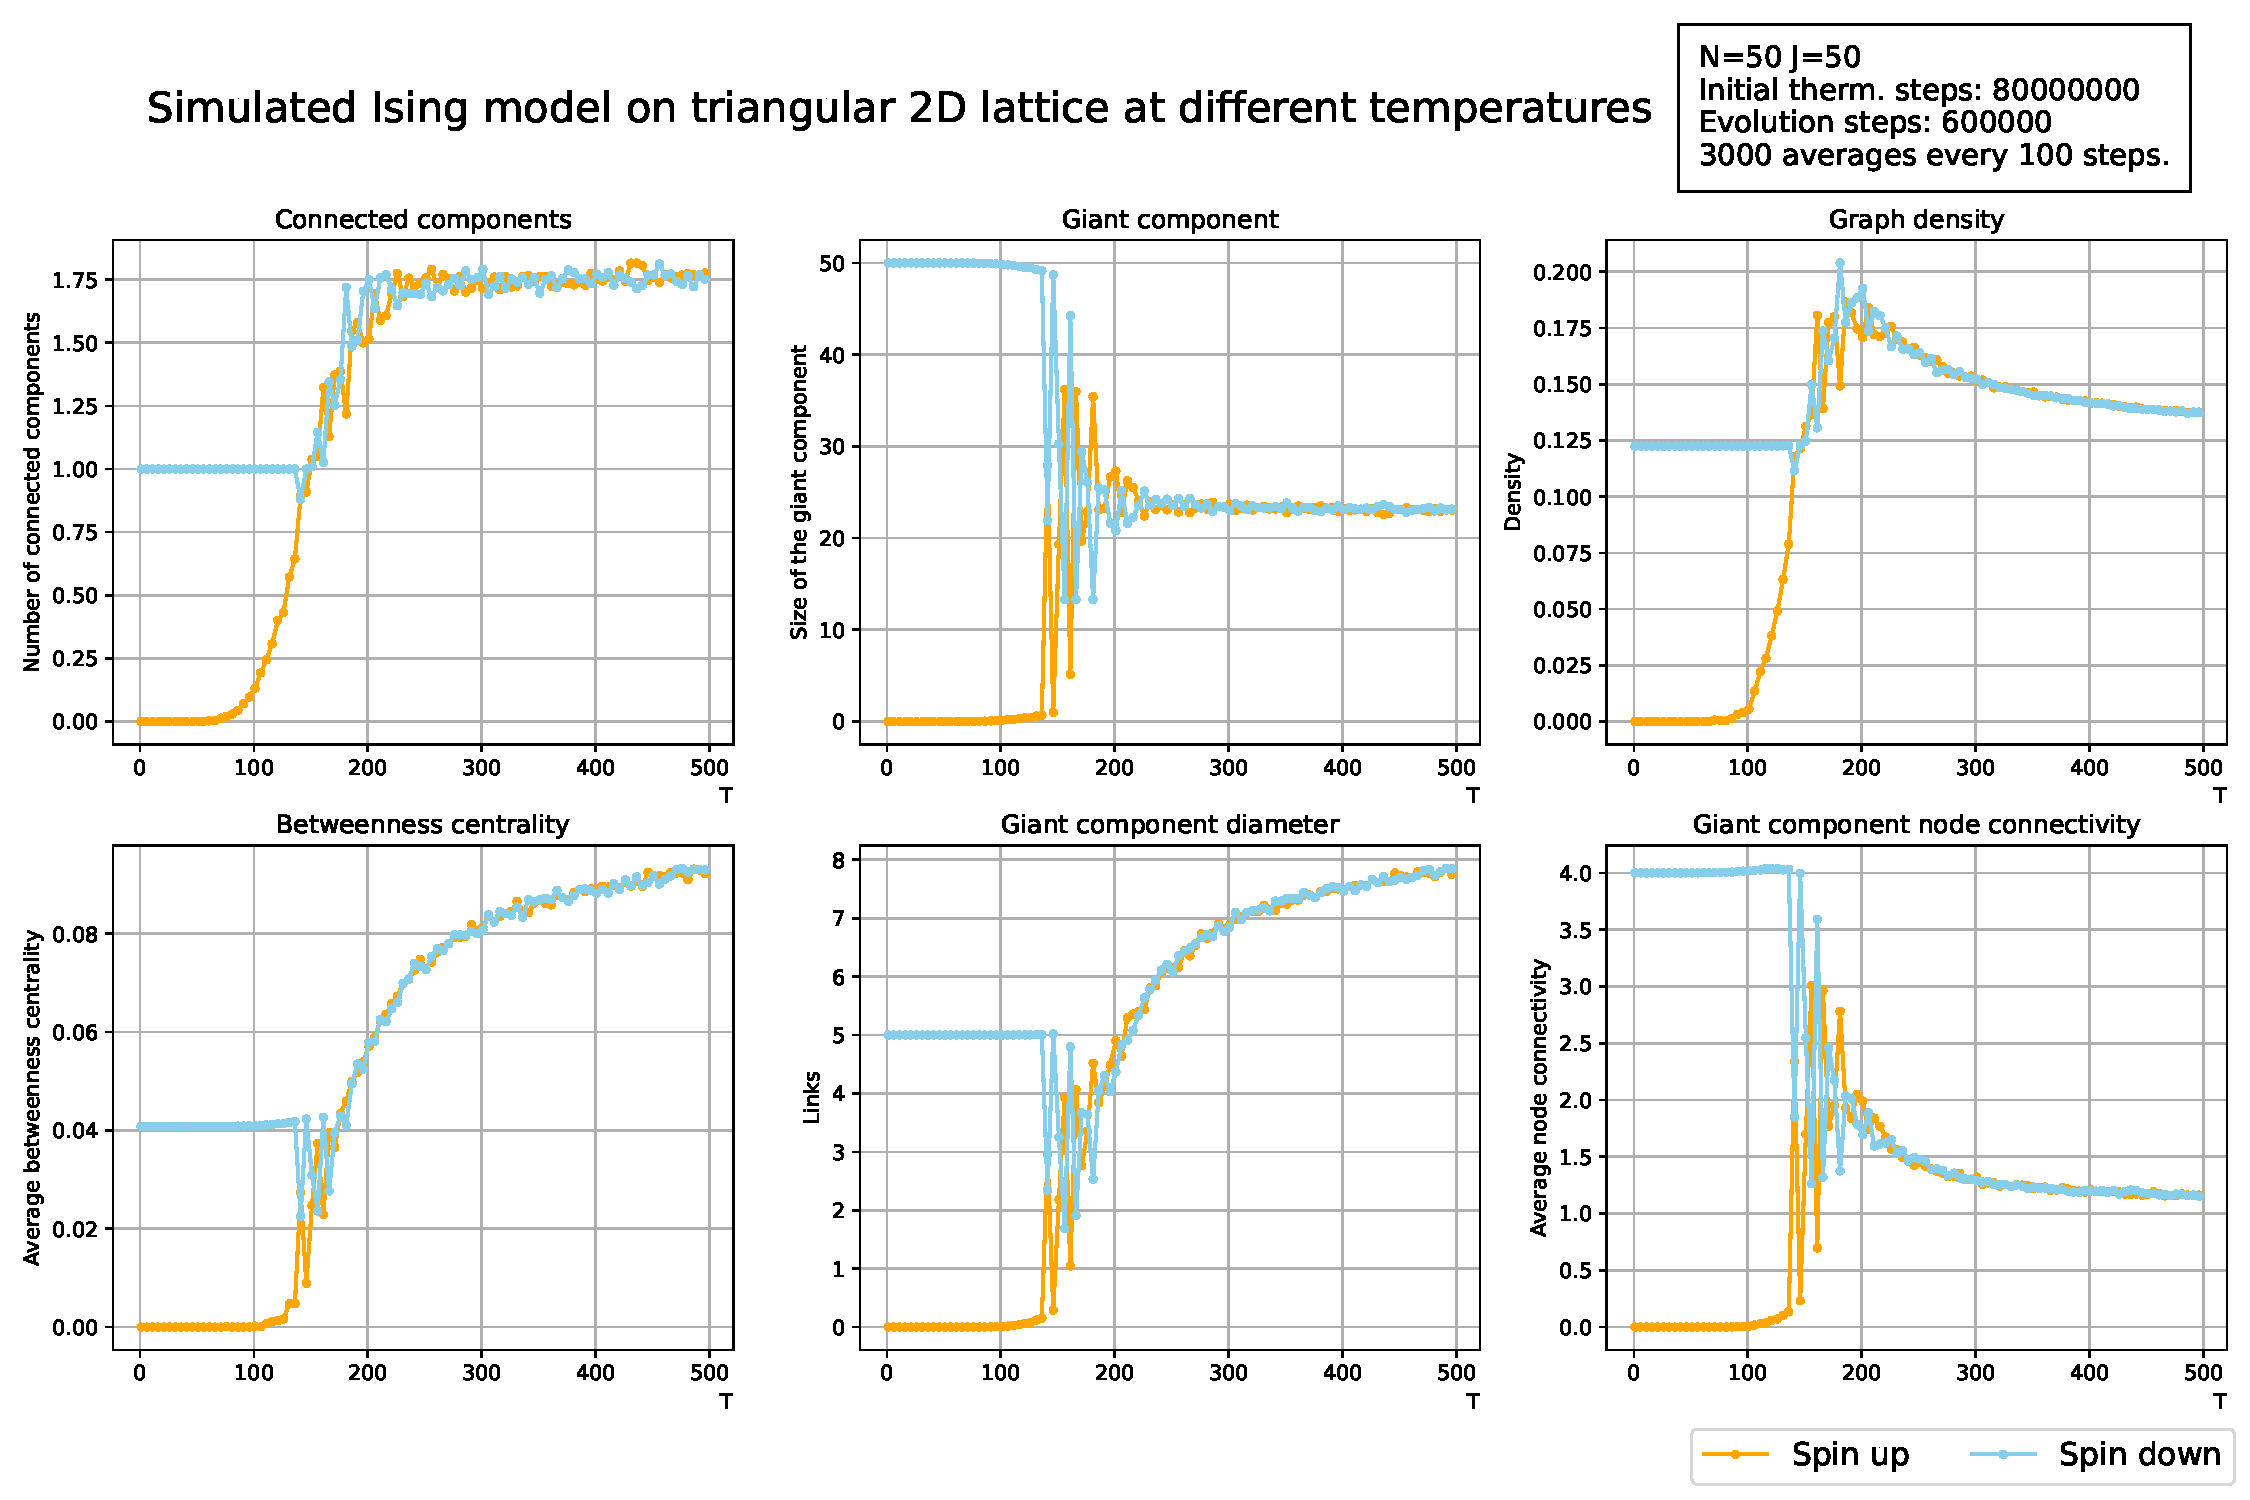
\includegraphics[width=.96\linewidth]{Network meausres/Triangular_Network.pdf}
    \caption{Behavior of the network proprieties of the triangular lattice at increasing temperatures. The orange line is the spin up network while the blue is the spin down one.}
    \label{Fig:triangularNetworkmeasure}
\end{figure}

\begin{figure}[!htb]
  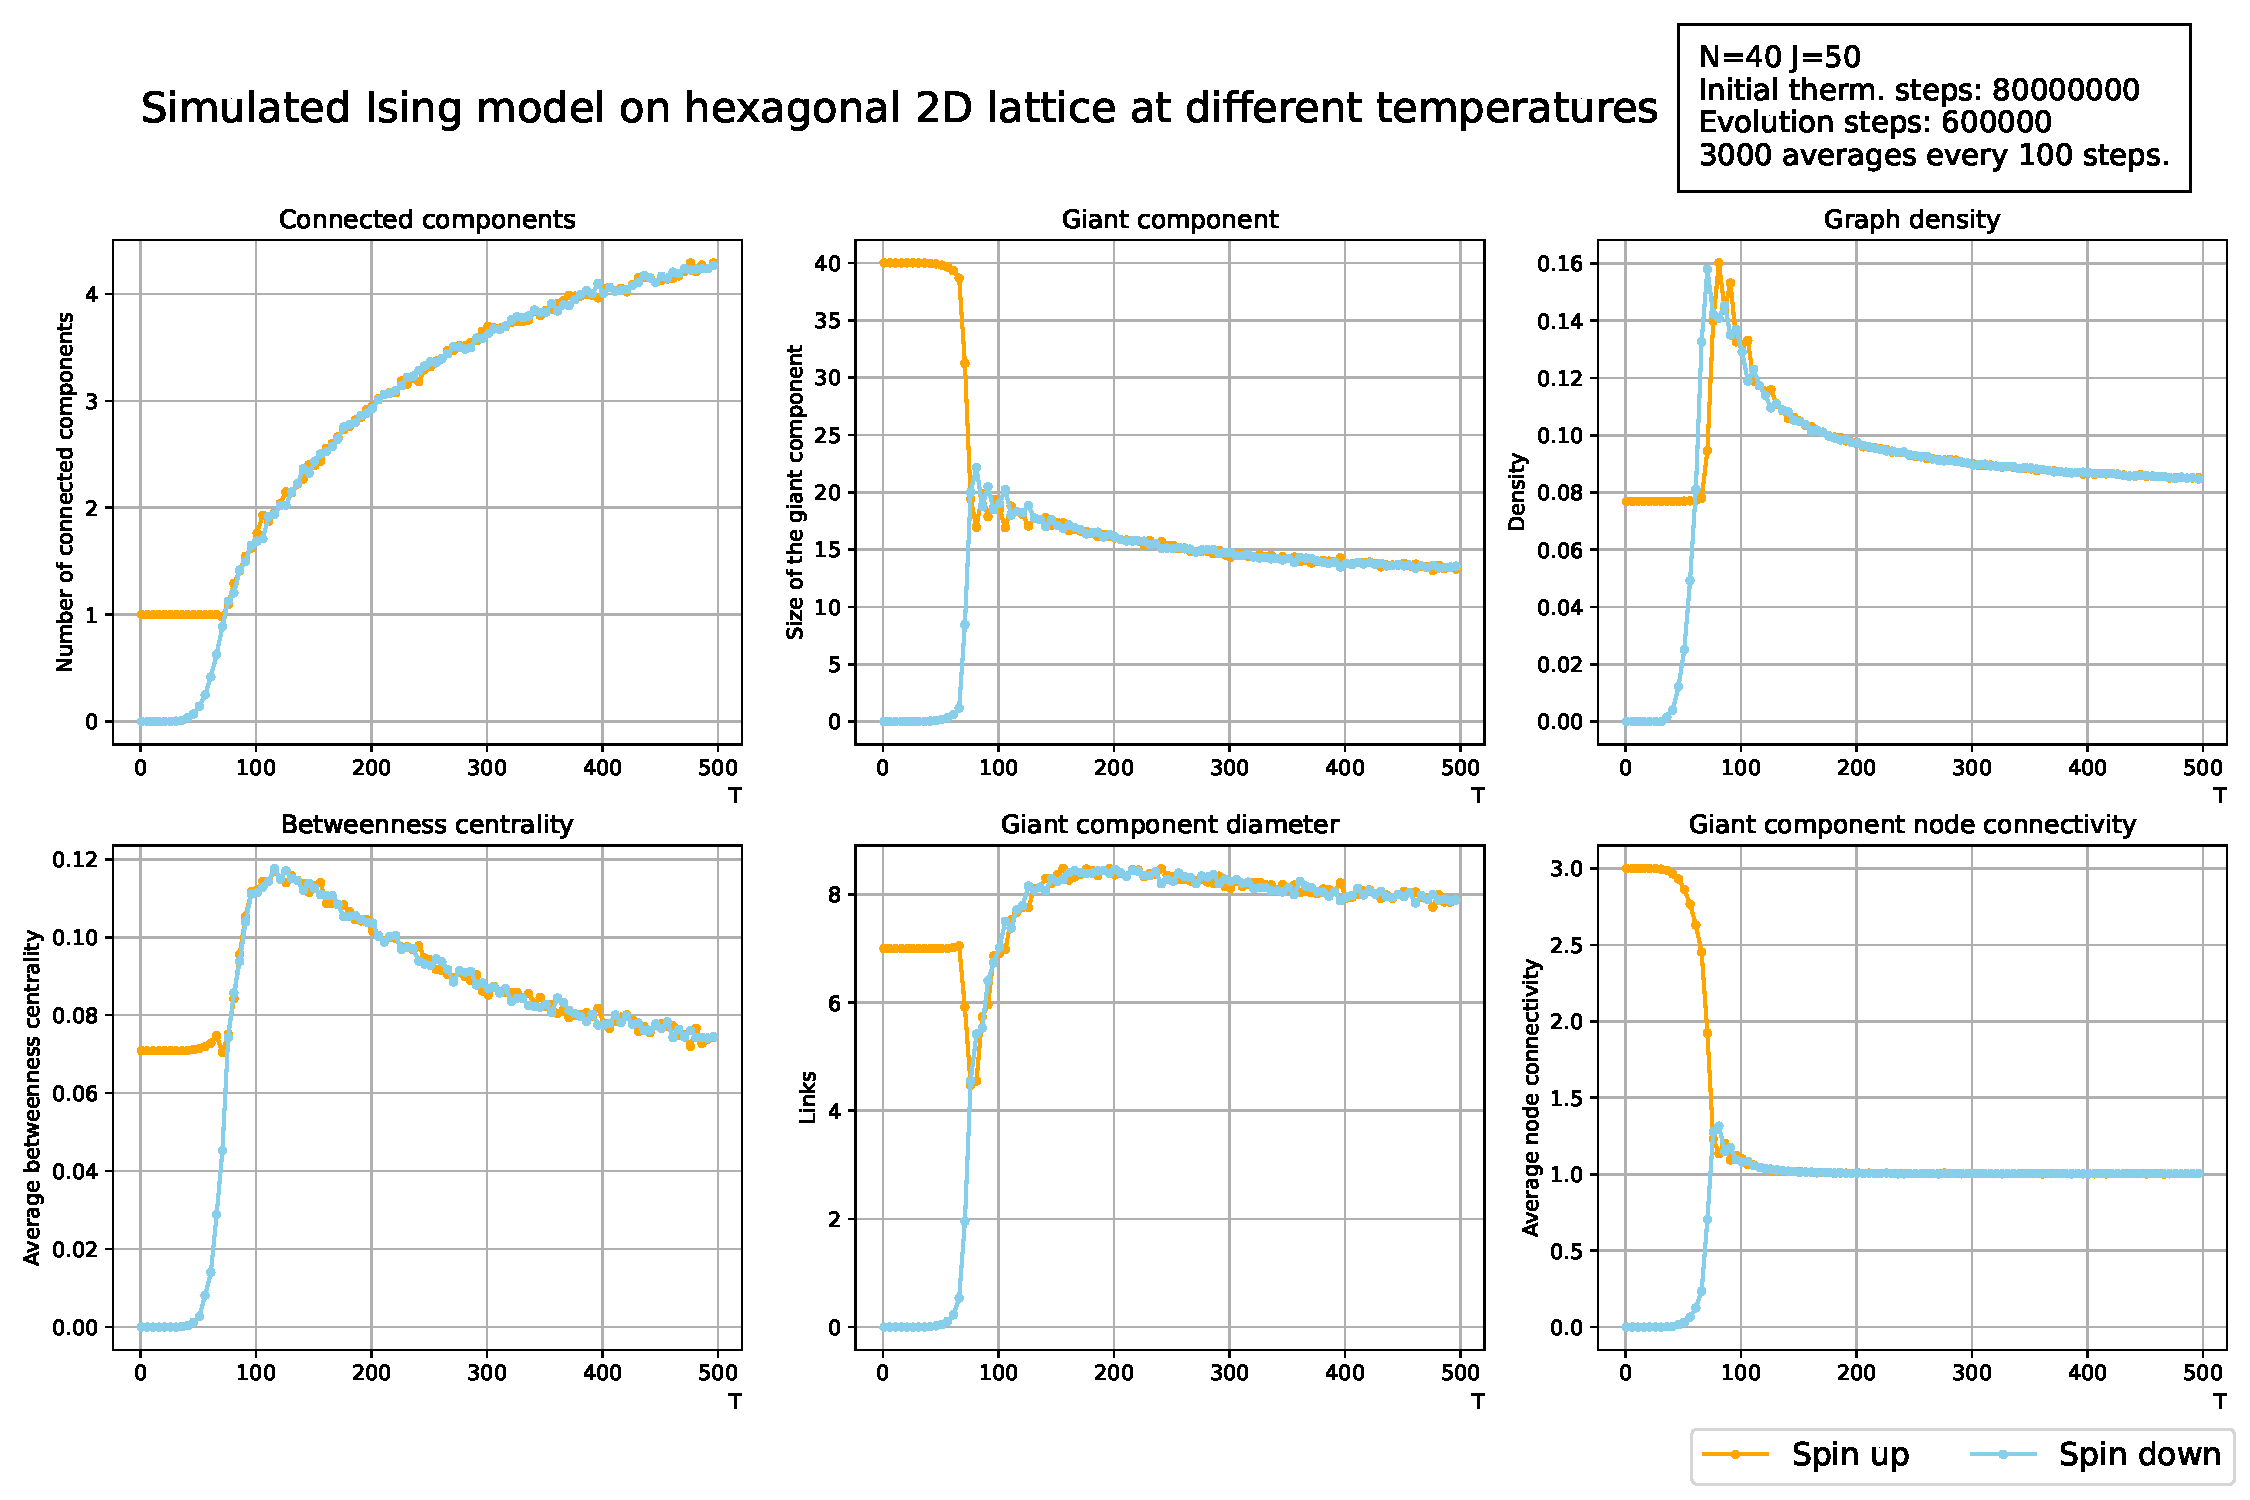
\includegraphics[width=.96\linewidth]{Network meausres/Hexagonal_Network.pdf}
    \caption{Behavior of the network proprieties of the hexagonal lattice at increasing temperatures. The orange line is the spin up network while the blue is the spin down one.}
    \label{Fig:hexagonalNetworkmeasure}
\end{figure}

Also the triangular and hexagonal lattices show the features we have just described. Figure \ref{Fig:triangularNetworkmeasure} shows that the triangular lattice breaks into fewer connected components with a slightly bigger giant compoents. Figure \ref{Fig:hexagonalNetworkmeasure} instead shows that hexagonal lattices break in more connected components, over 4, generating smaller giant components, with almost a third of atoms each. Furthermore, the hexagonal lattice shows an interesting behavior of the betweenness centrality: at the critical temperature it reaches a maximum point. This can be interpreted in the following way: first the network breaks into smaller components of a few atoms each with a higher betweenness centrality, however, then these smaller components start to become bigger and more connected and therefore their betweenness centrality drops.

\begin{figure}[!htb]
  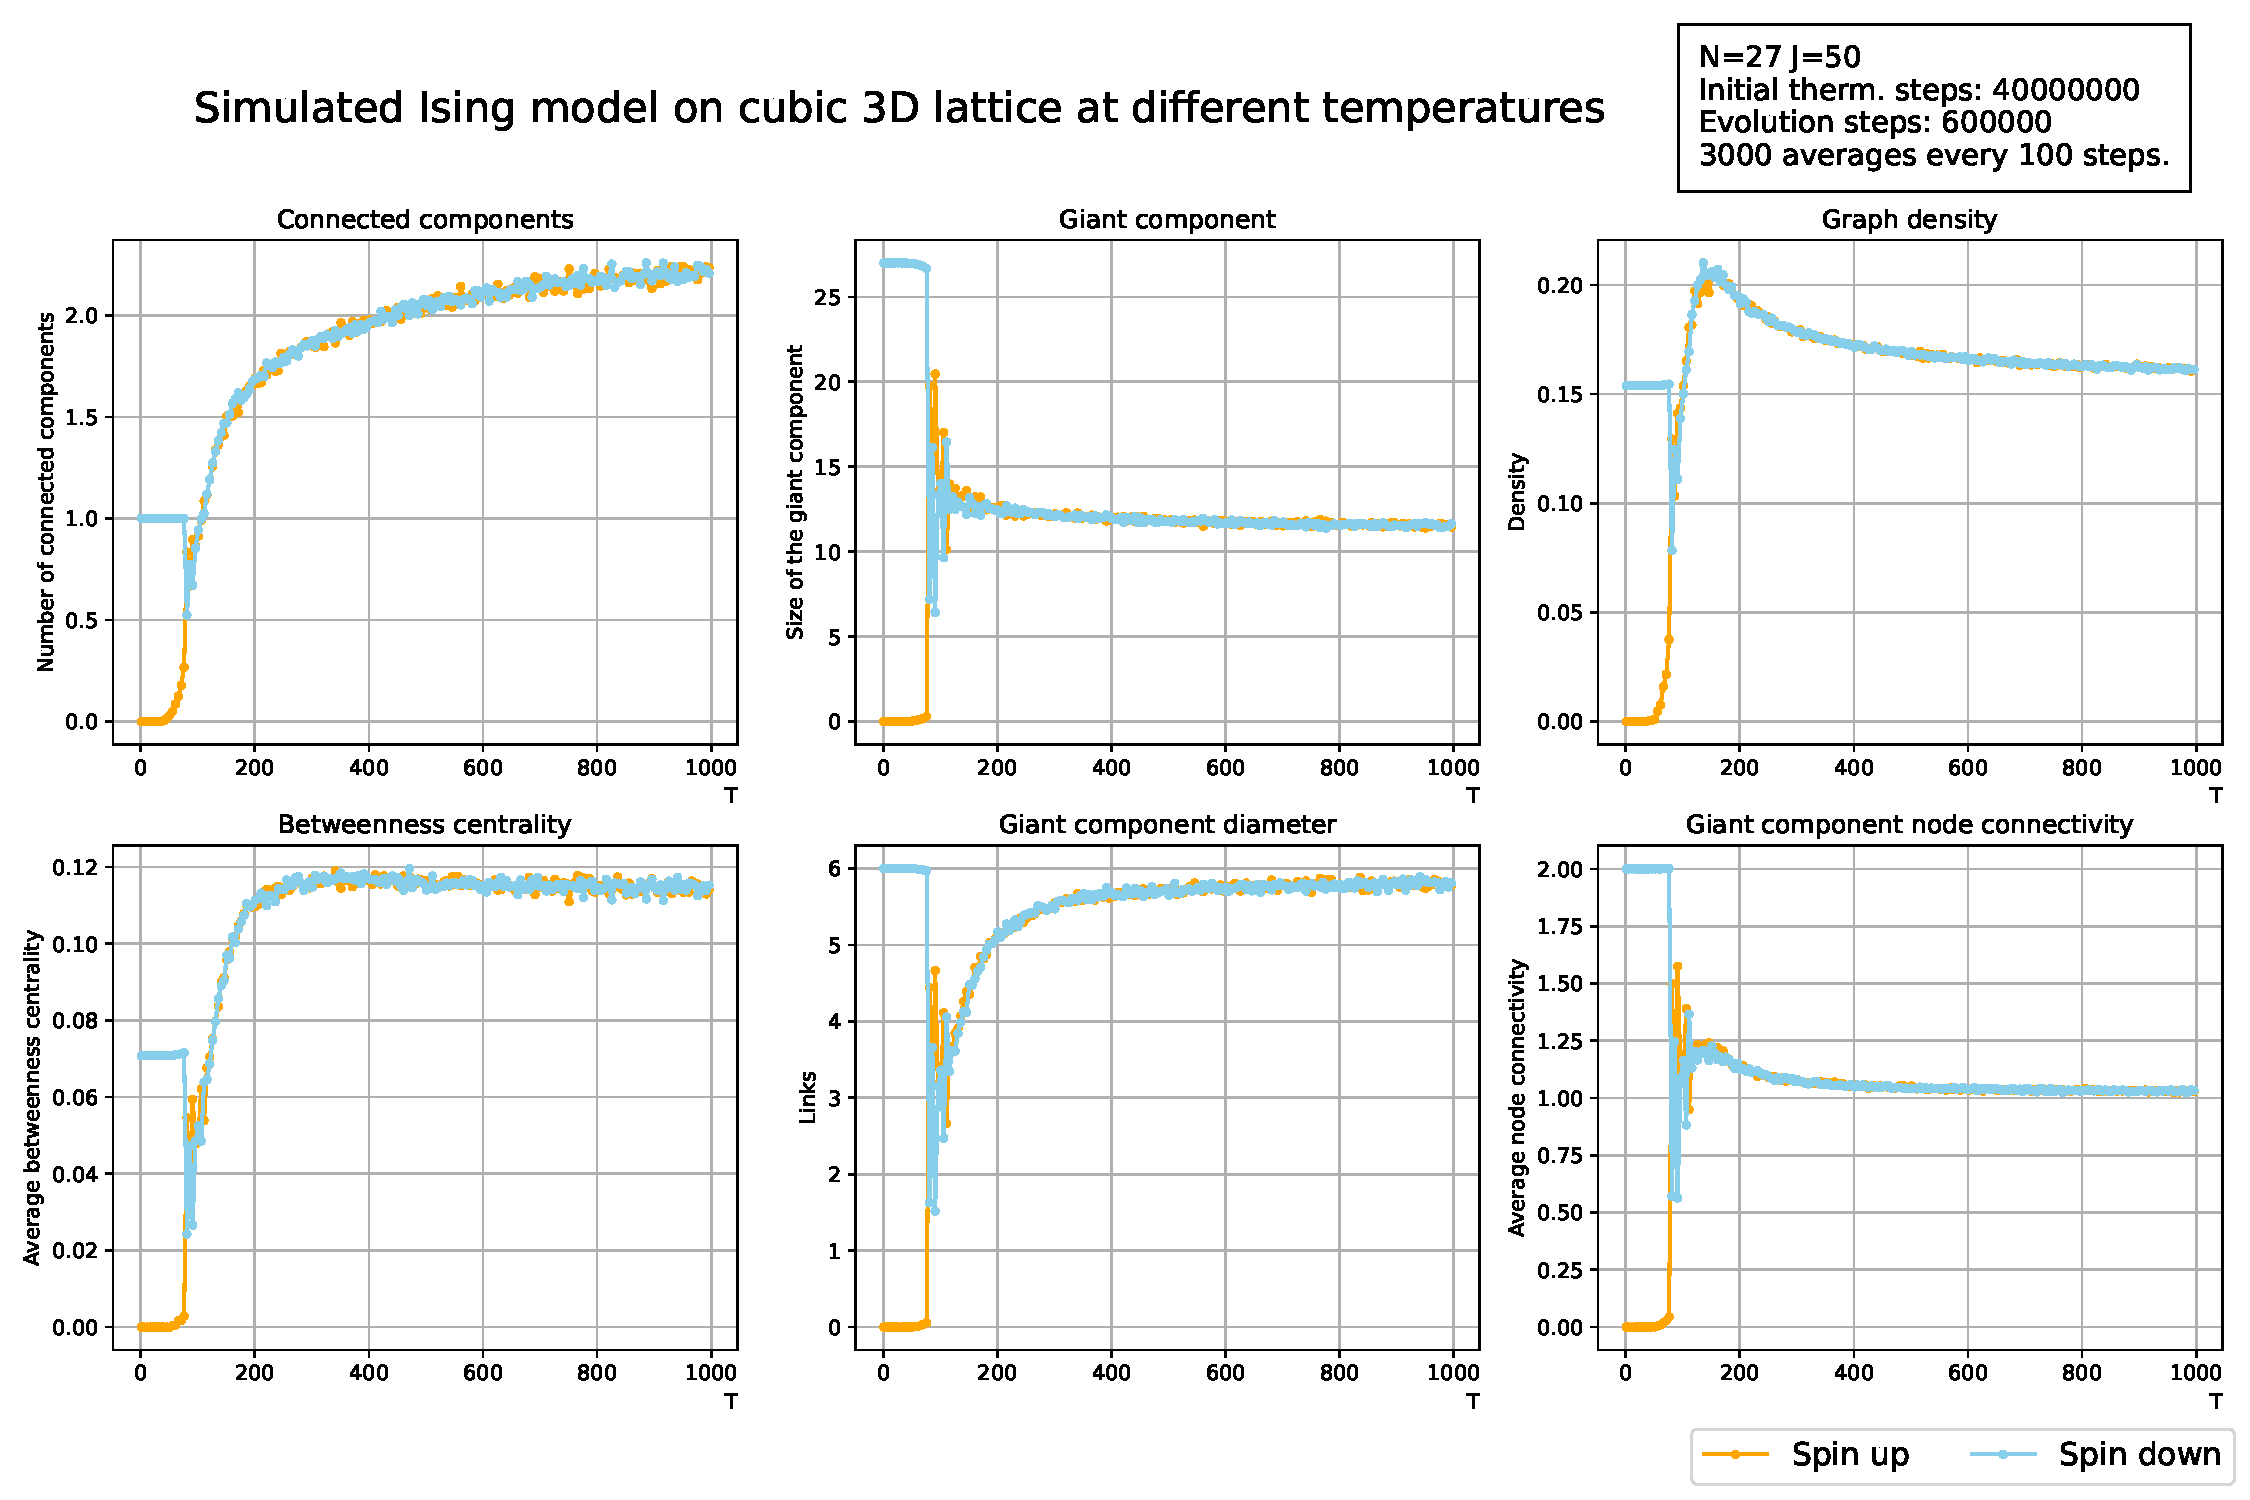
\includegraphics[width=\linewidth]{Network meausres/3D_Network.pdf}
    \caption{Behavior of the network proprieties of the 3D cubic lattice at increasing temperatures. The orange line is the spin up network while the blue is the spin down one.}
    \label{Fig:3DNetworkmeasure}
\end{figure}

The last analysis we conducted is on the 3D cubic lattice: this is shown in Figure \ref{Fig:3DNetworkmeasure}. The same behavior of the previous networks is again showed by the 3D cubic lattice, however it is interesting to note that in this case the diameter of the giant component, after its drop during the phase transition, slowly rises again approaching $6$ links, which is the diameter of the all aligned lattice at $T=0$.

Another interesting observation that emerges from these graphs is that, even though we analyzed 4 different types of networks in different dimension, staring from different average node connectivity all converges to 1 after the phase transition. This shows that, independently of the network proprieties, all aligned spins networks become a tree graph. 

\subsection{Exotic networks}
In this last section we will analyze some exotic kind of networks that we tried to simulate.
\subsubsection*{Broken lattices}
Networks with some fraction of atoms removed (broken) could mimic the behavior of lattices with defects: for this reason we simulated a square lattice of 100 atoms from which we started to remove some fractions of atoms. Form Figure \ref{Fig:BSNetworkmeasure} we can see that as we increase the number of removed atoms the phase transition is still manifest, however the critical temperature starts to change: with only 5 atoms removed the giant component starts to break at around $T=100$ while with 30 atoms removed it happens just after $T=50$. This is not unexpected, since removing atoms we also decrease the number of interactions, from the mean field approximation critical temperature $T_C=JZ$, we can see that lowering the number of links we decrease the critical temperature. Another interesting behavior we observe is that after the phase transition, as we remove atoms, the number of connected component raises: in every simulation we start 1 connected component but then we are left at $T=200$ with around 4 connected components per spin type, for lattices with fewer removed atoms, to over 7 components after the removal of one third of the atoms. As we could expect the size of the giant components get lowered, almost halved. This indicates that as we add defects the atoms struggle more to create magnetic domains. Lastly we observed, during the simulation, that the thermalization time, as we increase the number of removed atoms, increased too. For this reason we could just remove up to 30 atoms.
\begin{figure}[!htb]
\end{figure}
\begin{figure}[!htb]
  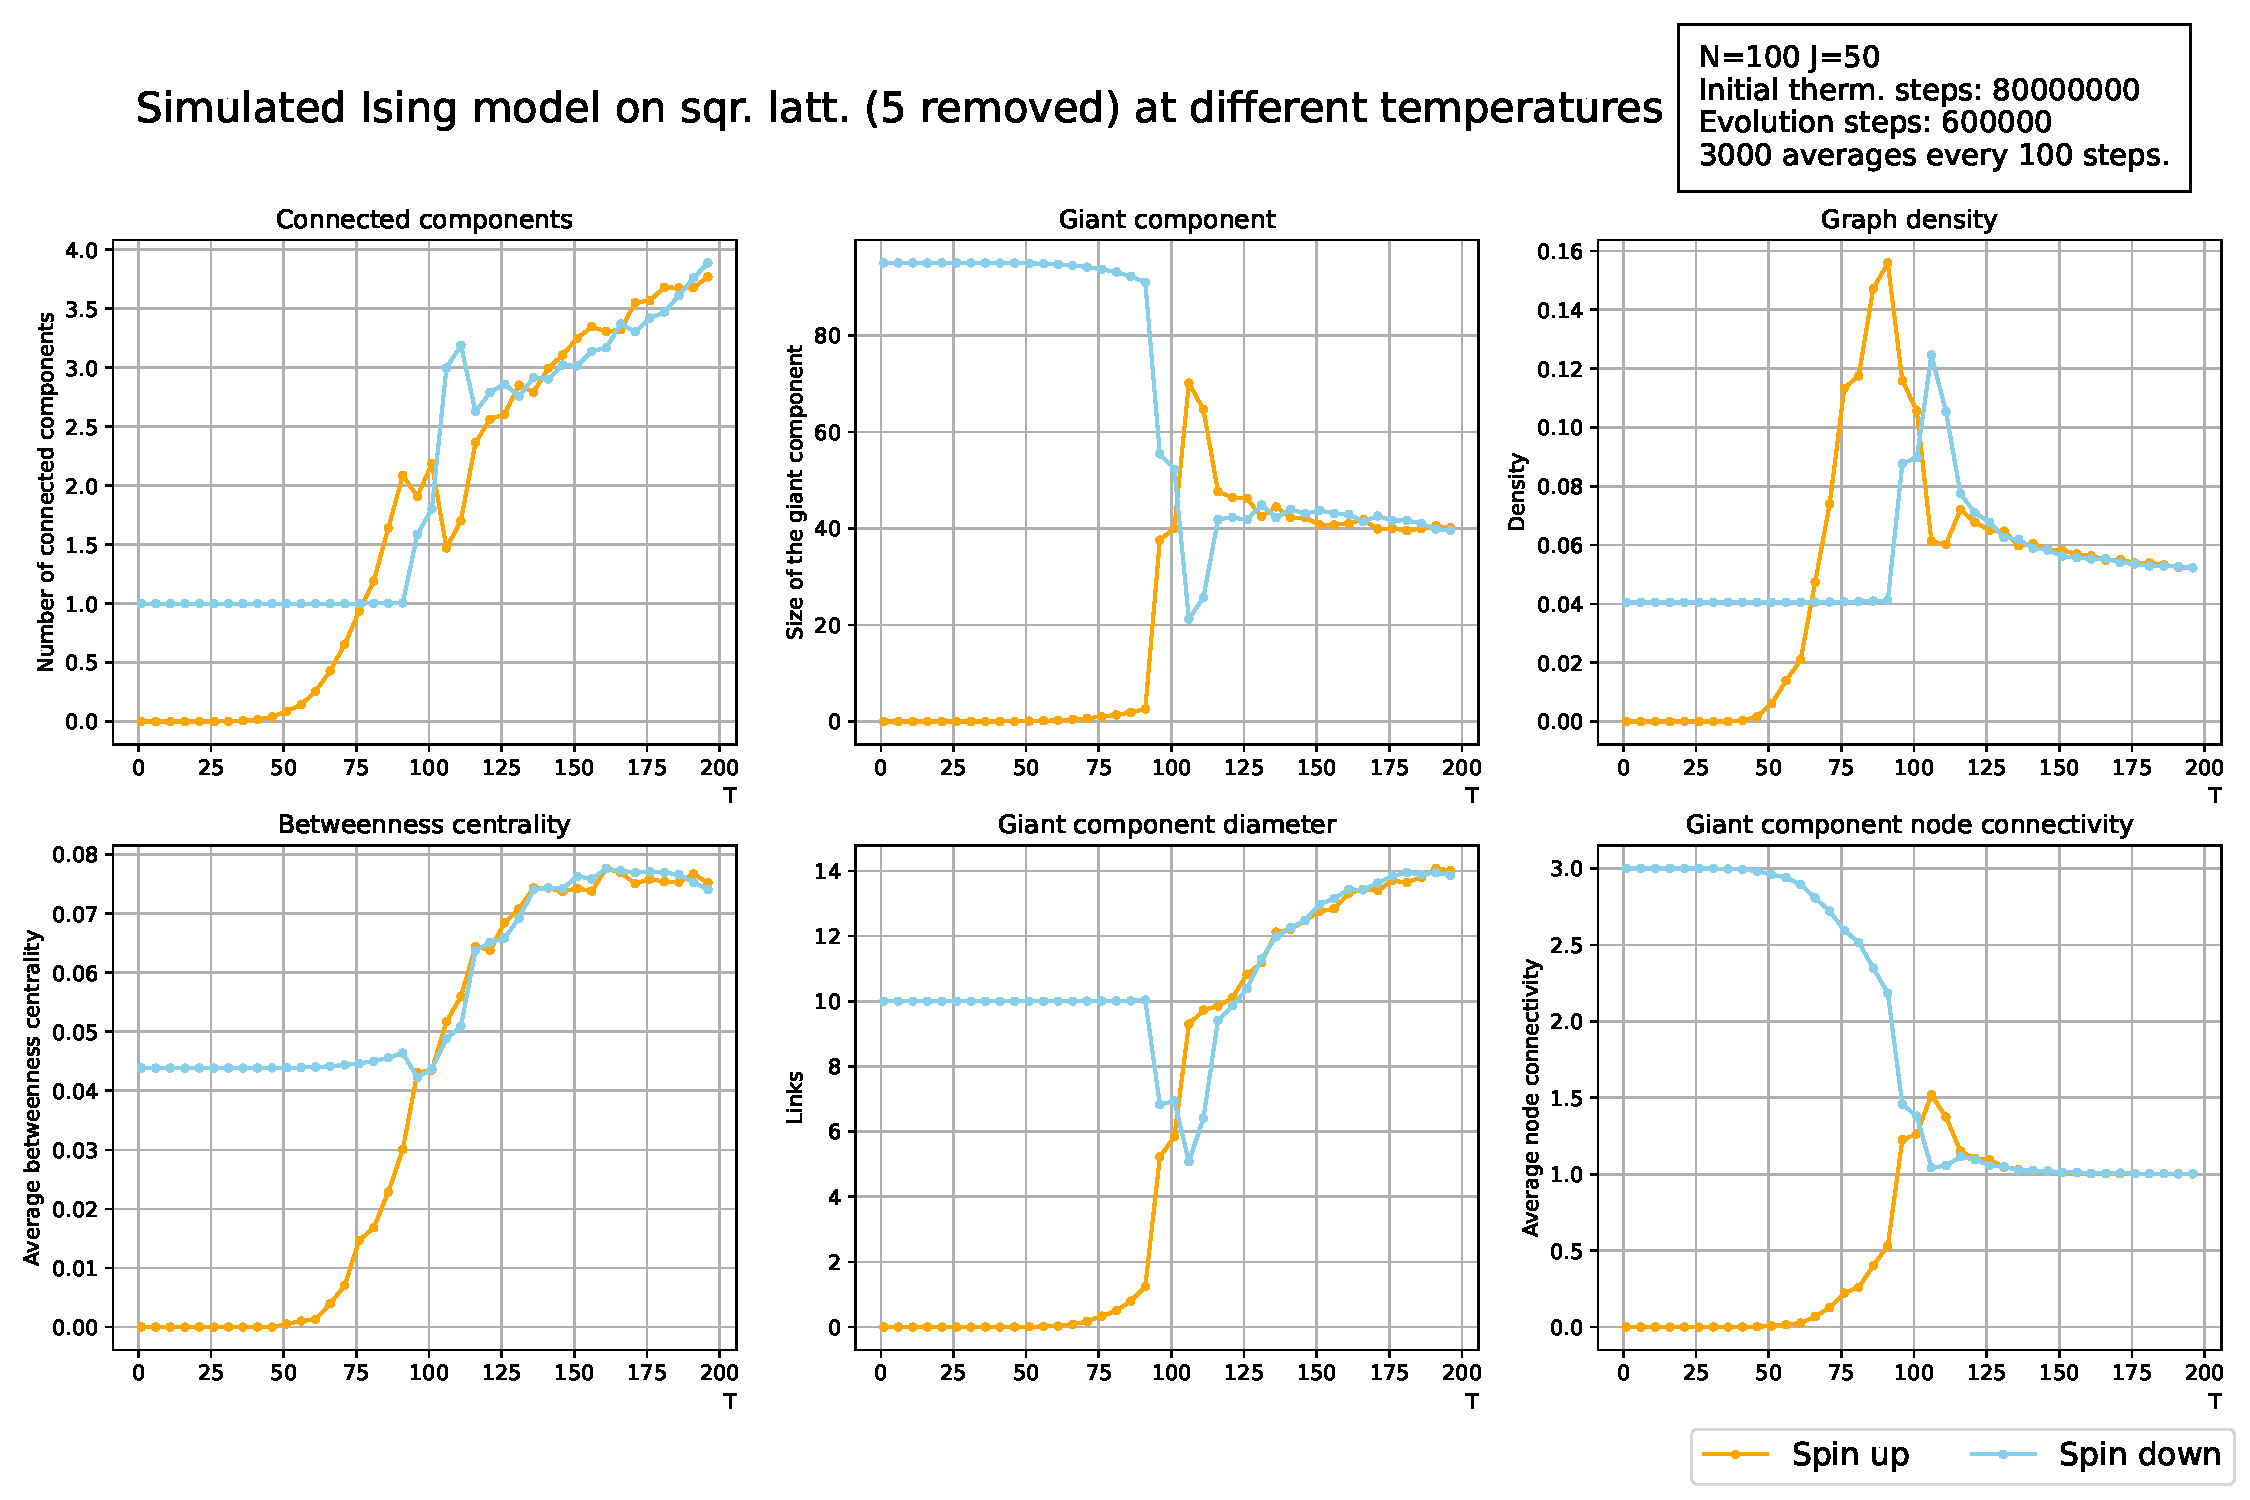
\includegraphics[width=.5\linewidth]{Broken/Figure_5.pdf}
  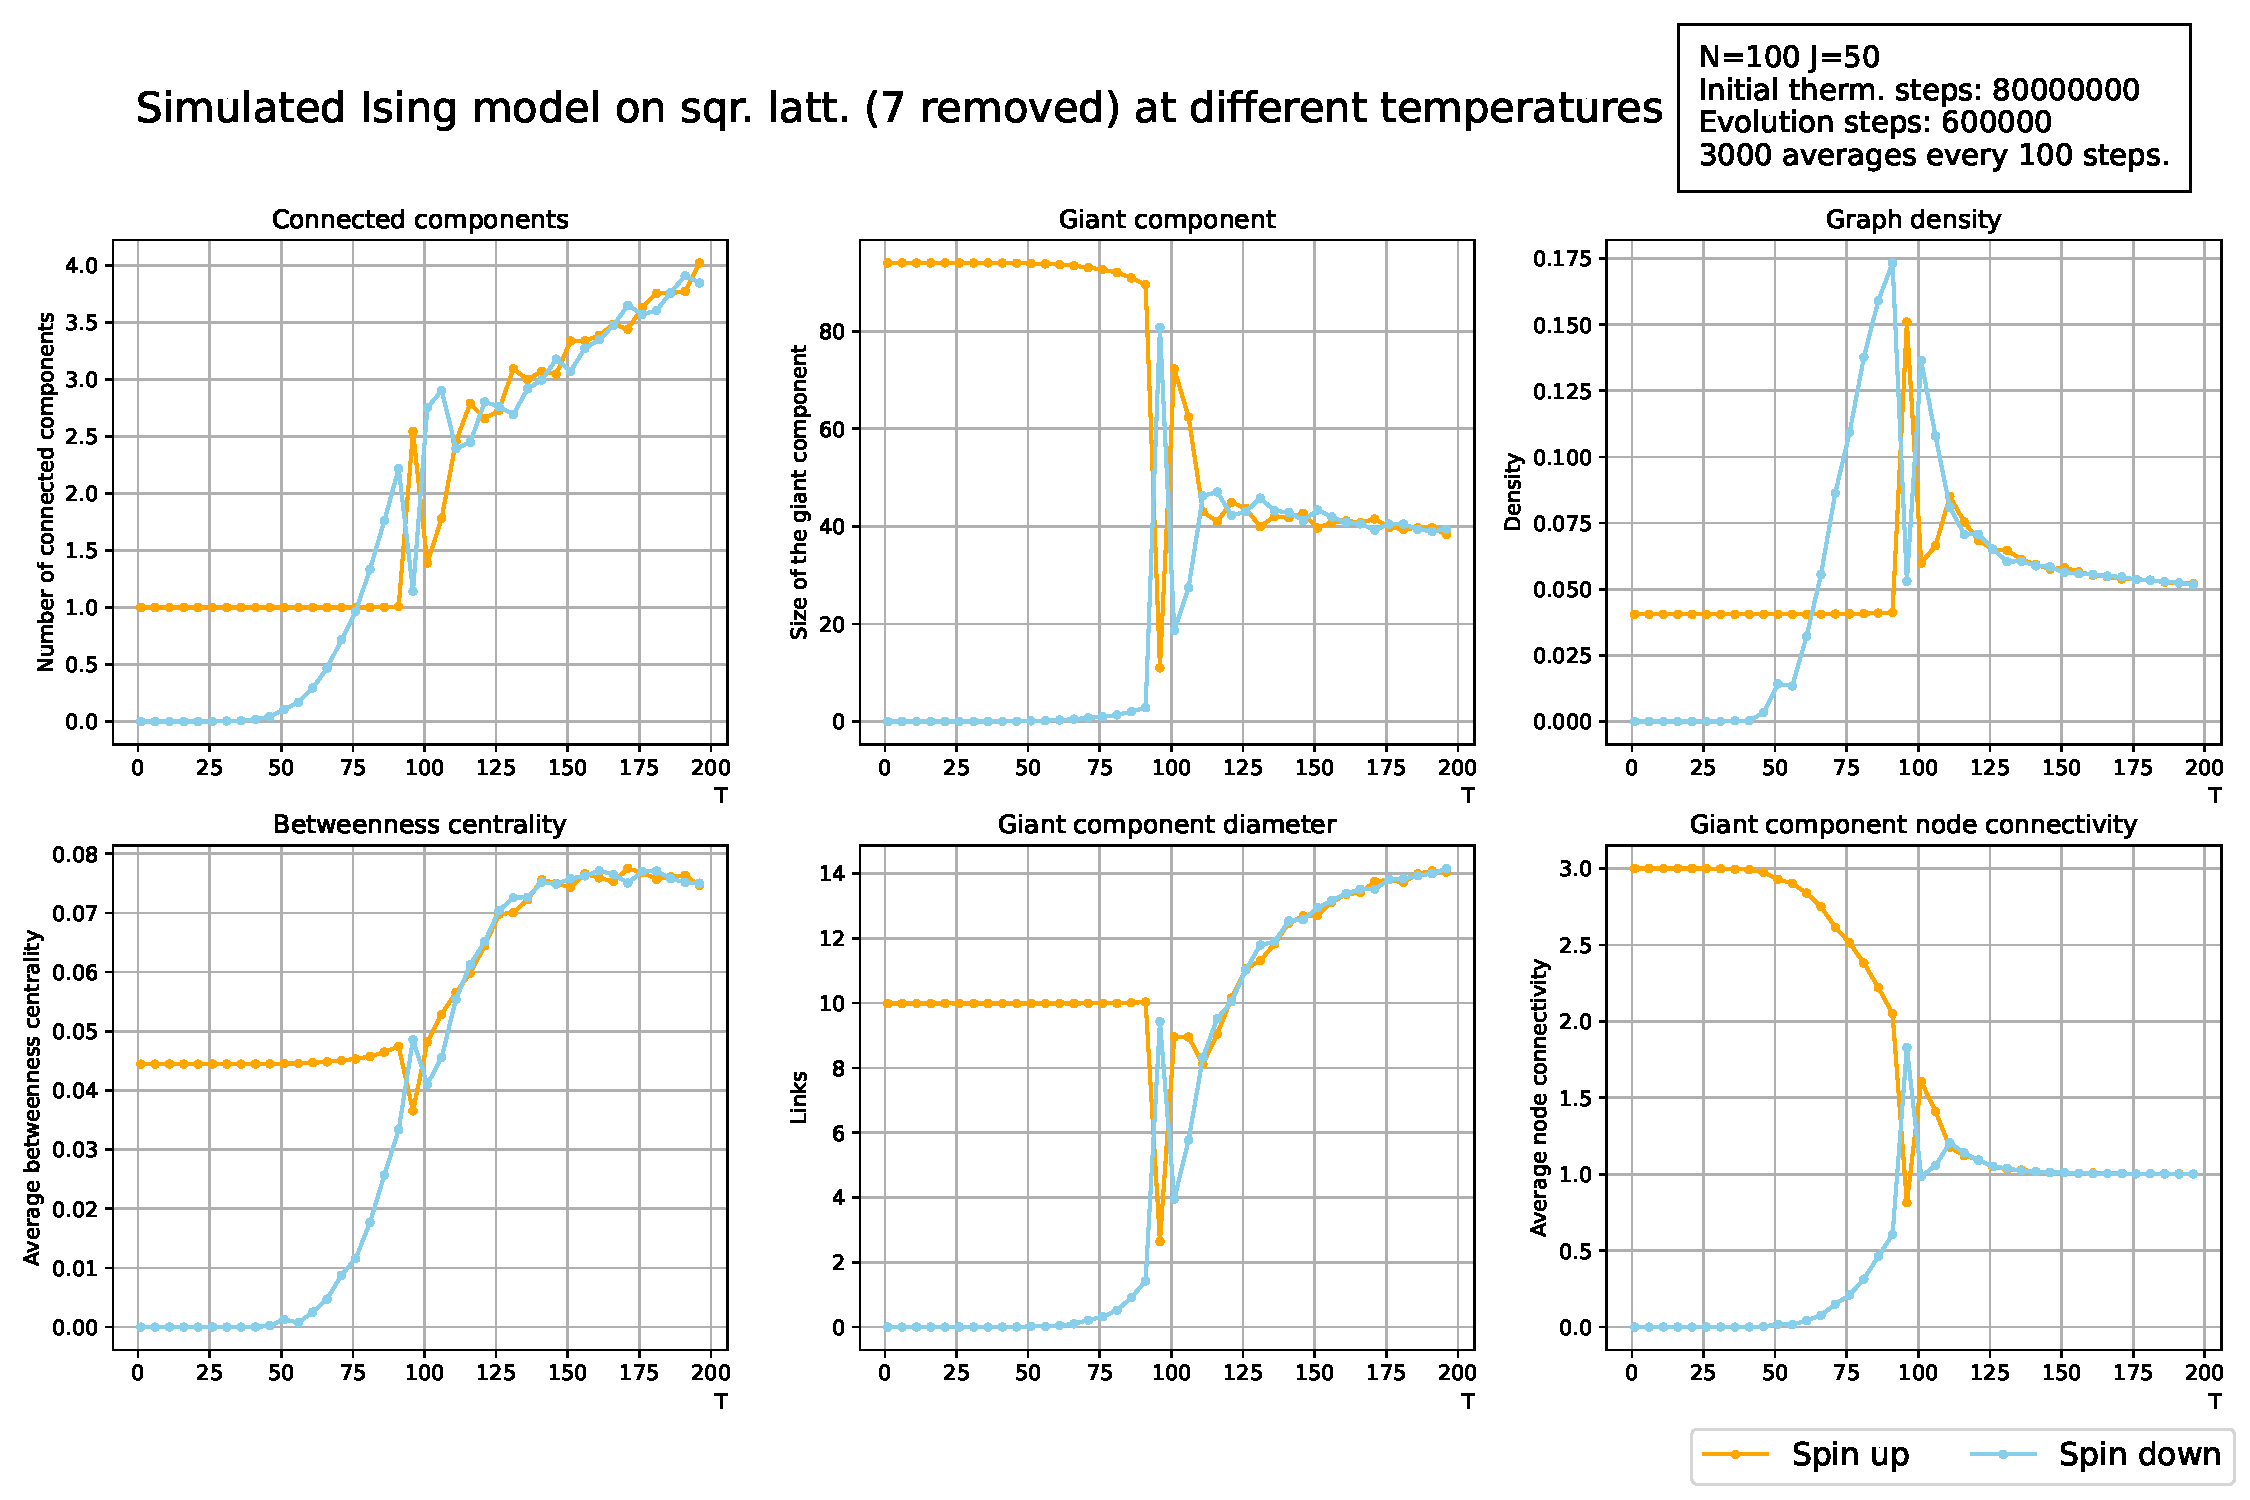
\includegraphics[width=.5\linewidth]{Broken/Square_7.pdf}

  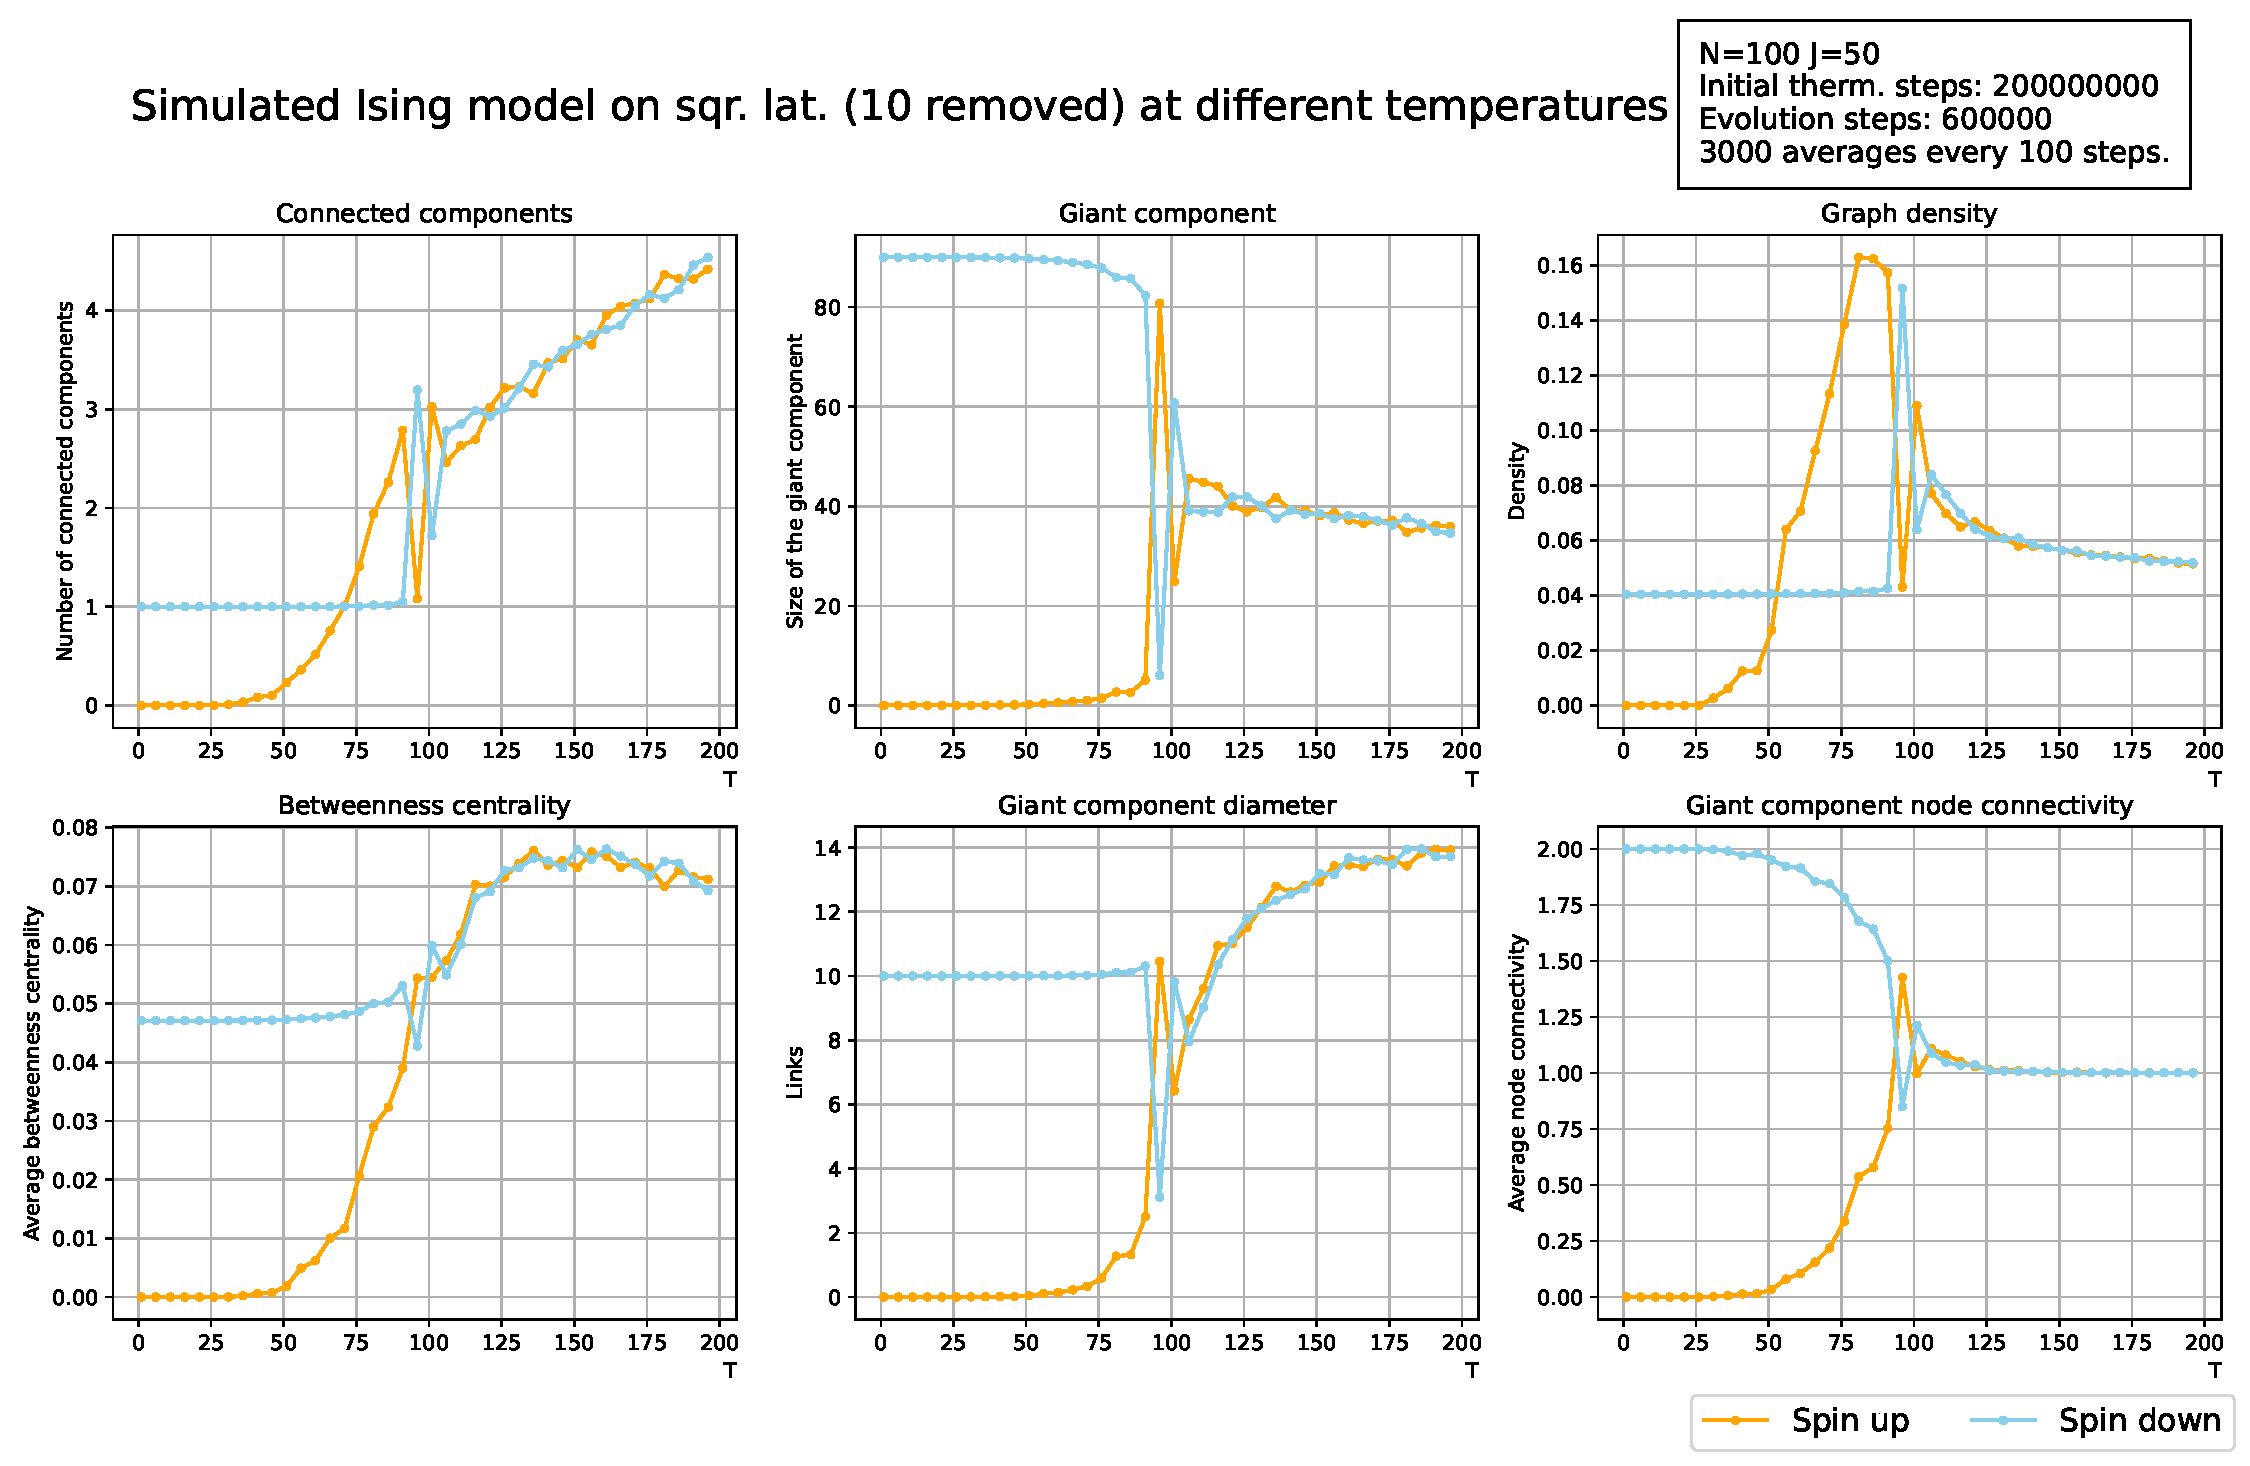
\includegraphics[width=.5\linewidth]{Broken/Square_10.pdf}
  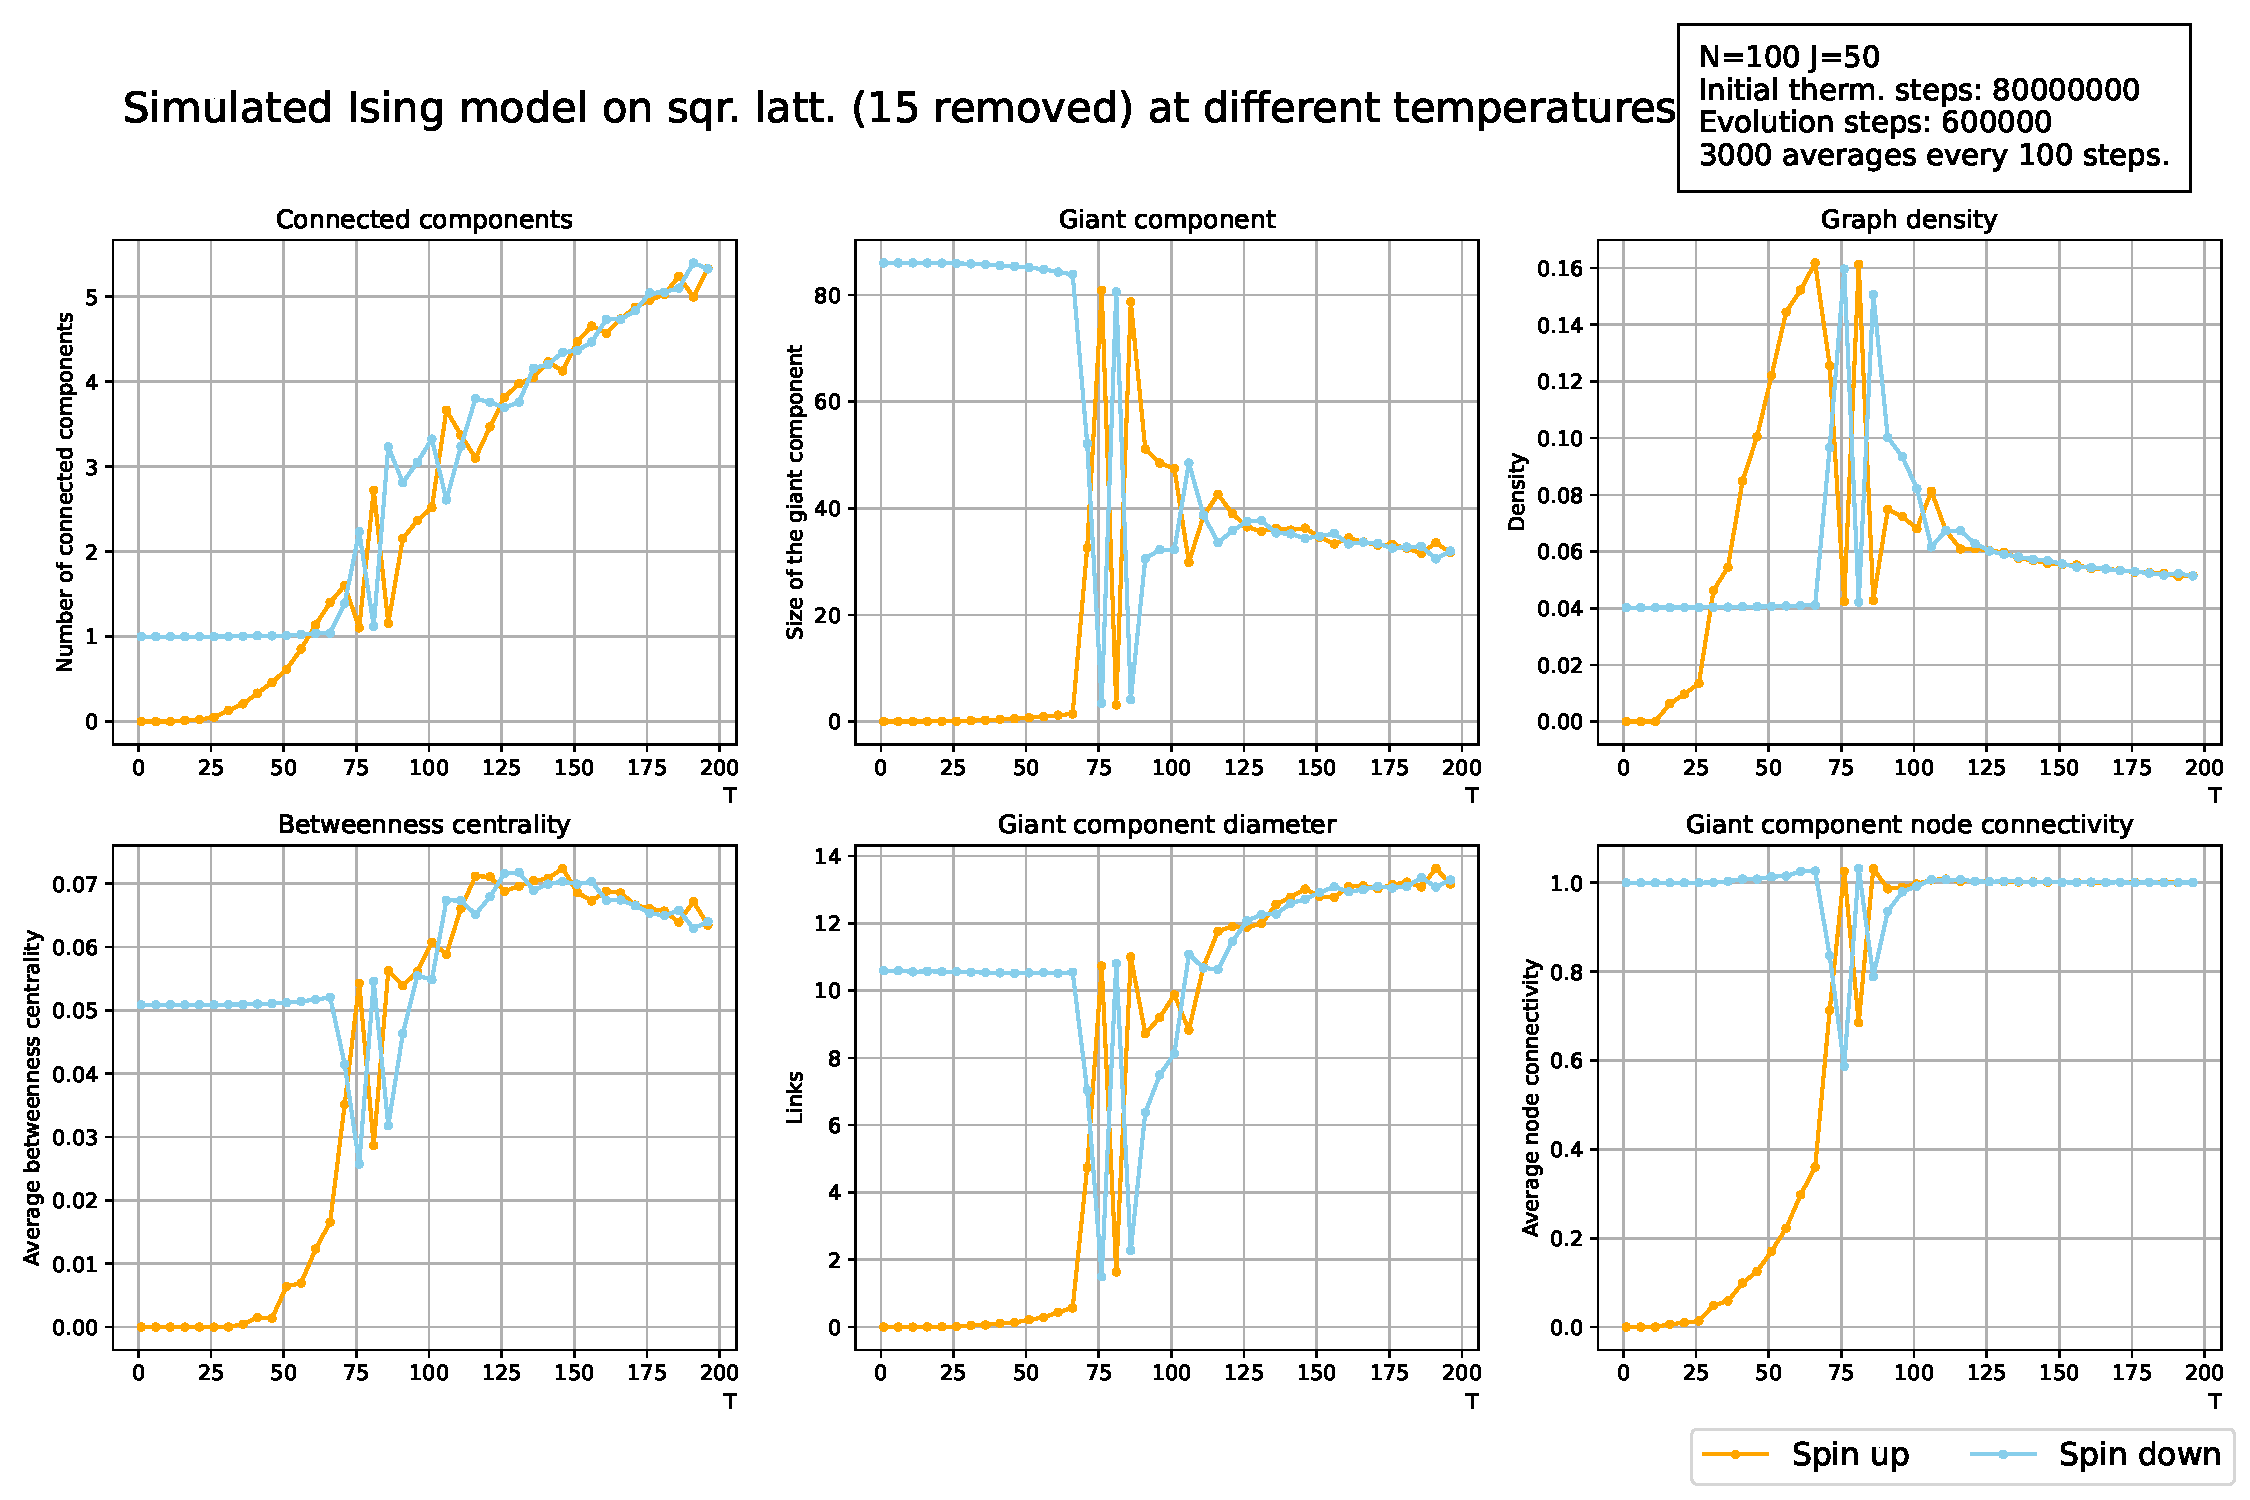
\includegraphics[width=.5\linewidth]{Broken/Square_15.pdf}

  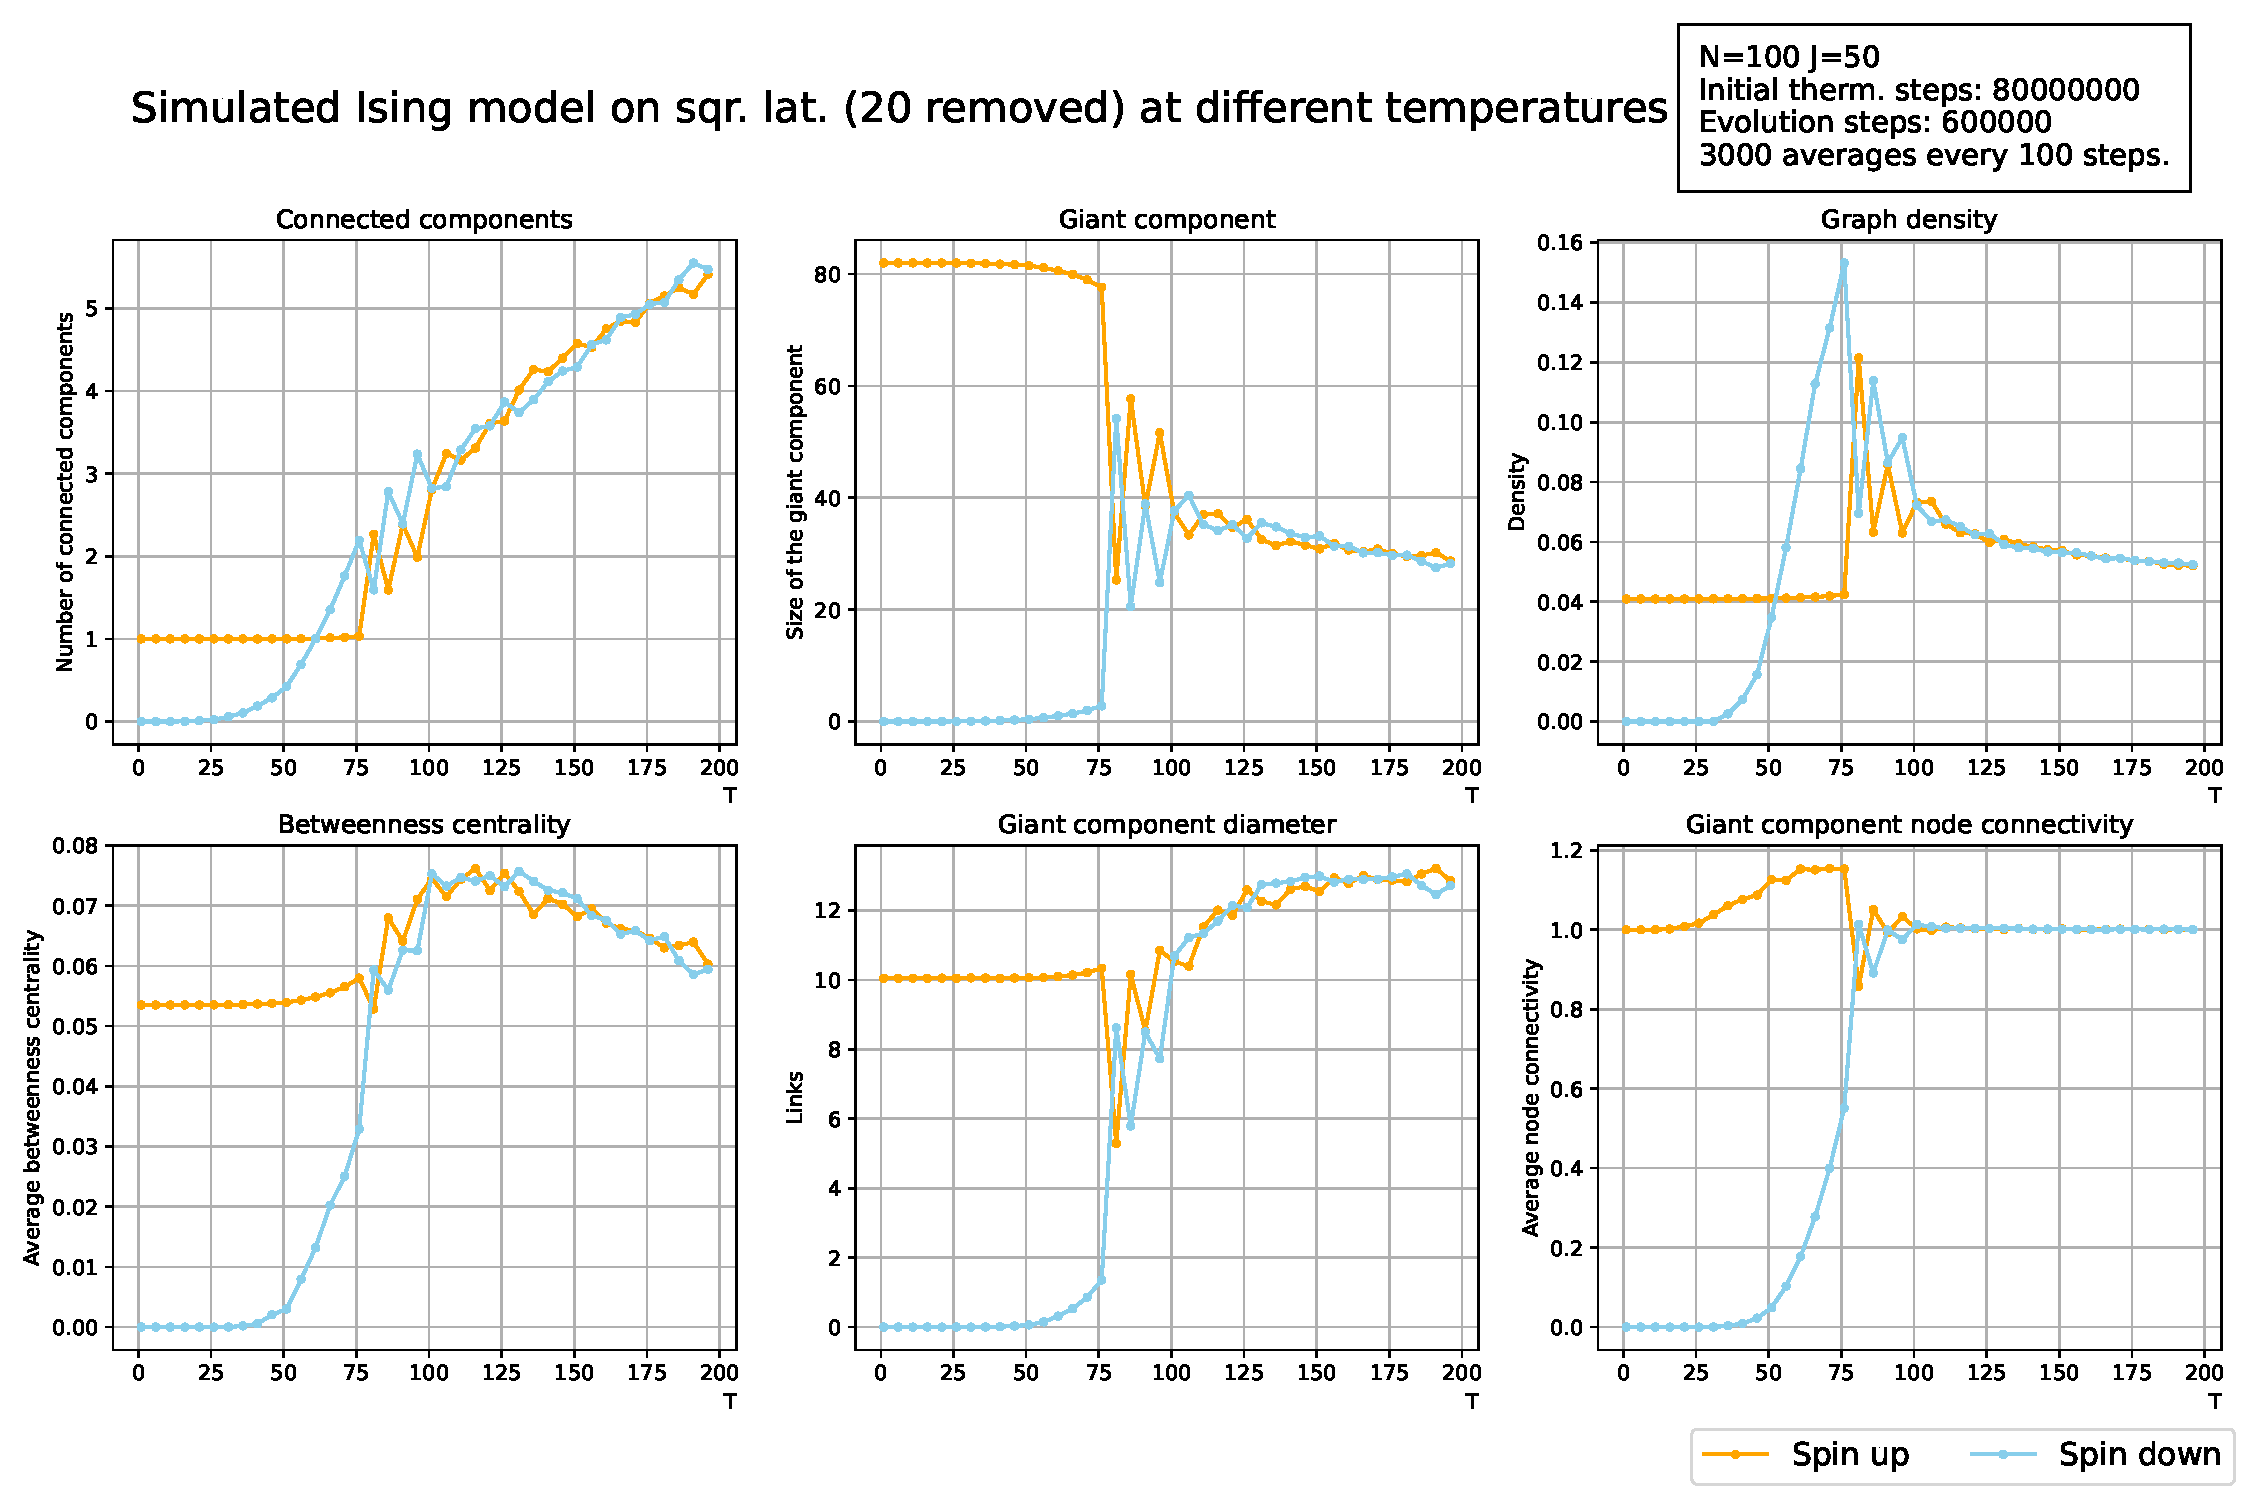
\includegraphics[width=.5\linewidth]{Broken/Square_20.pdf}
  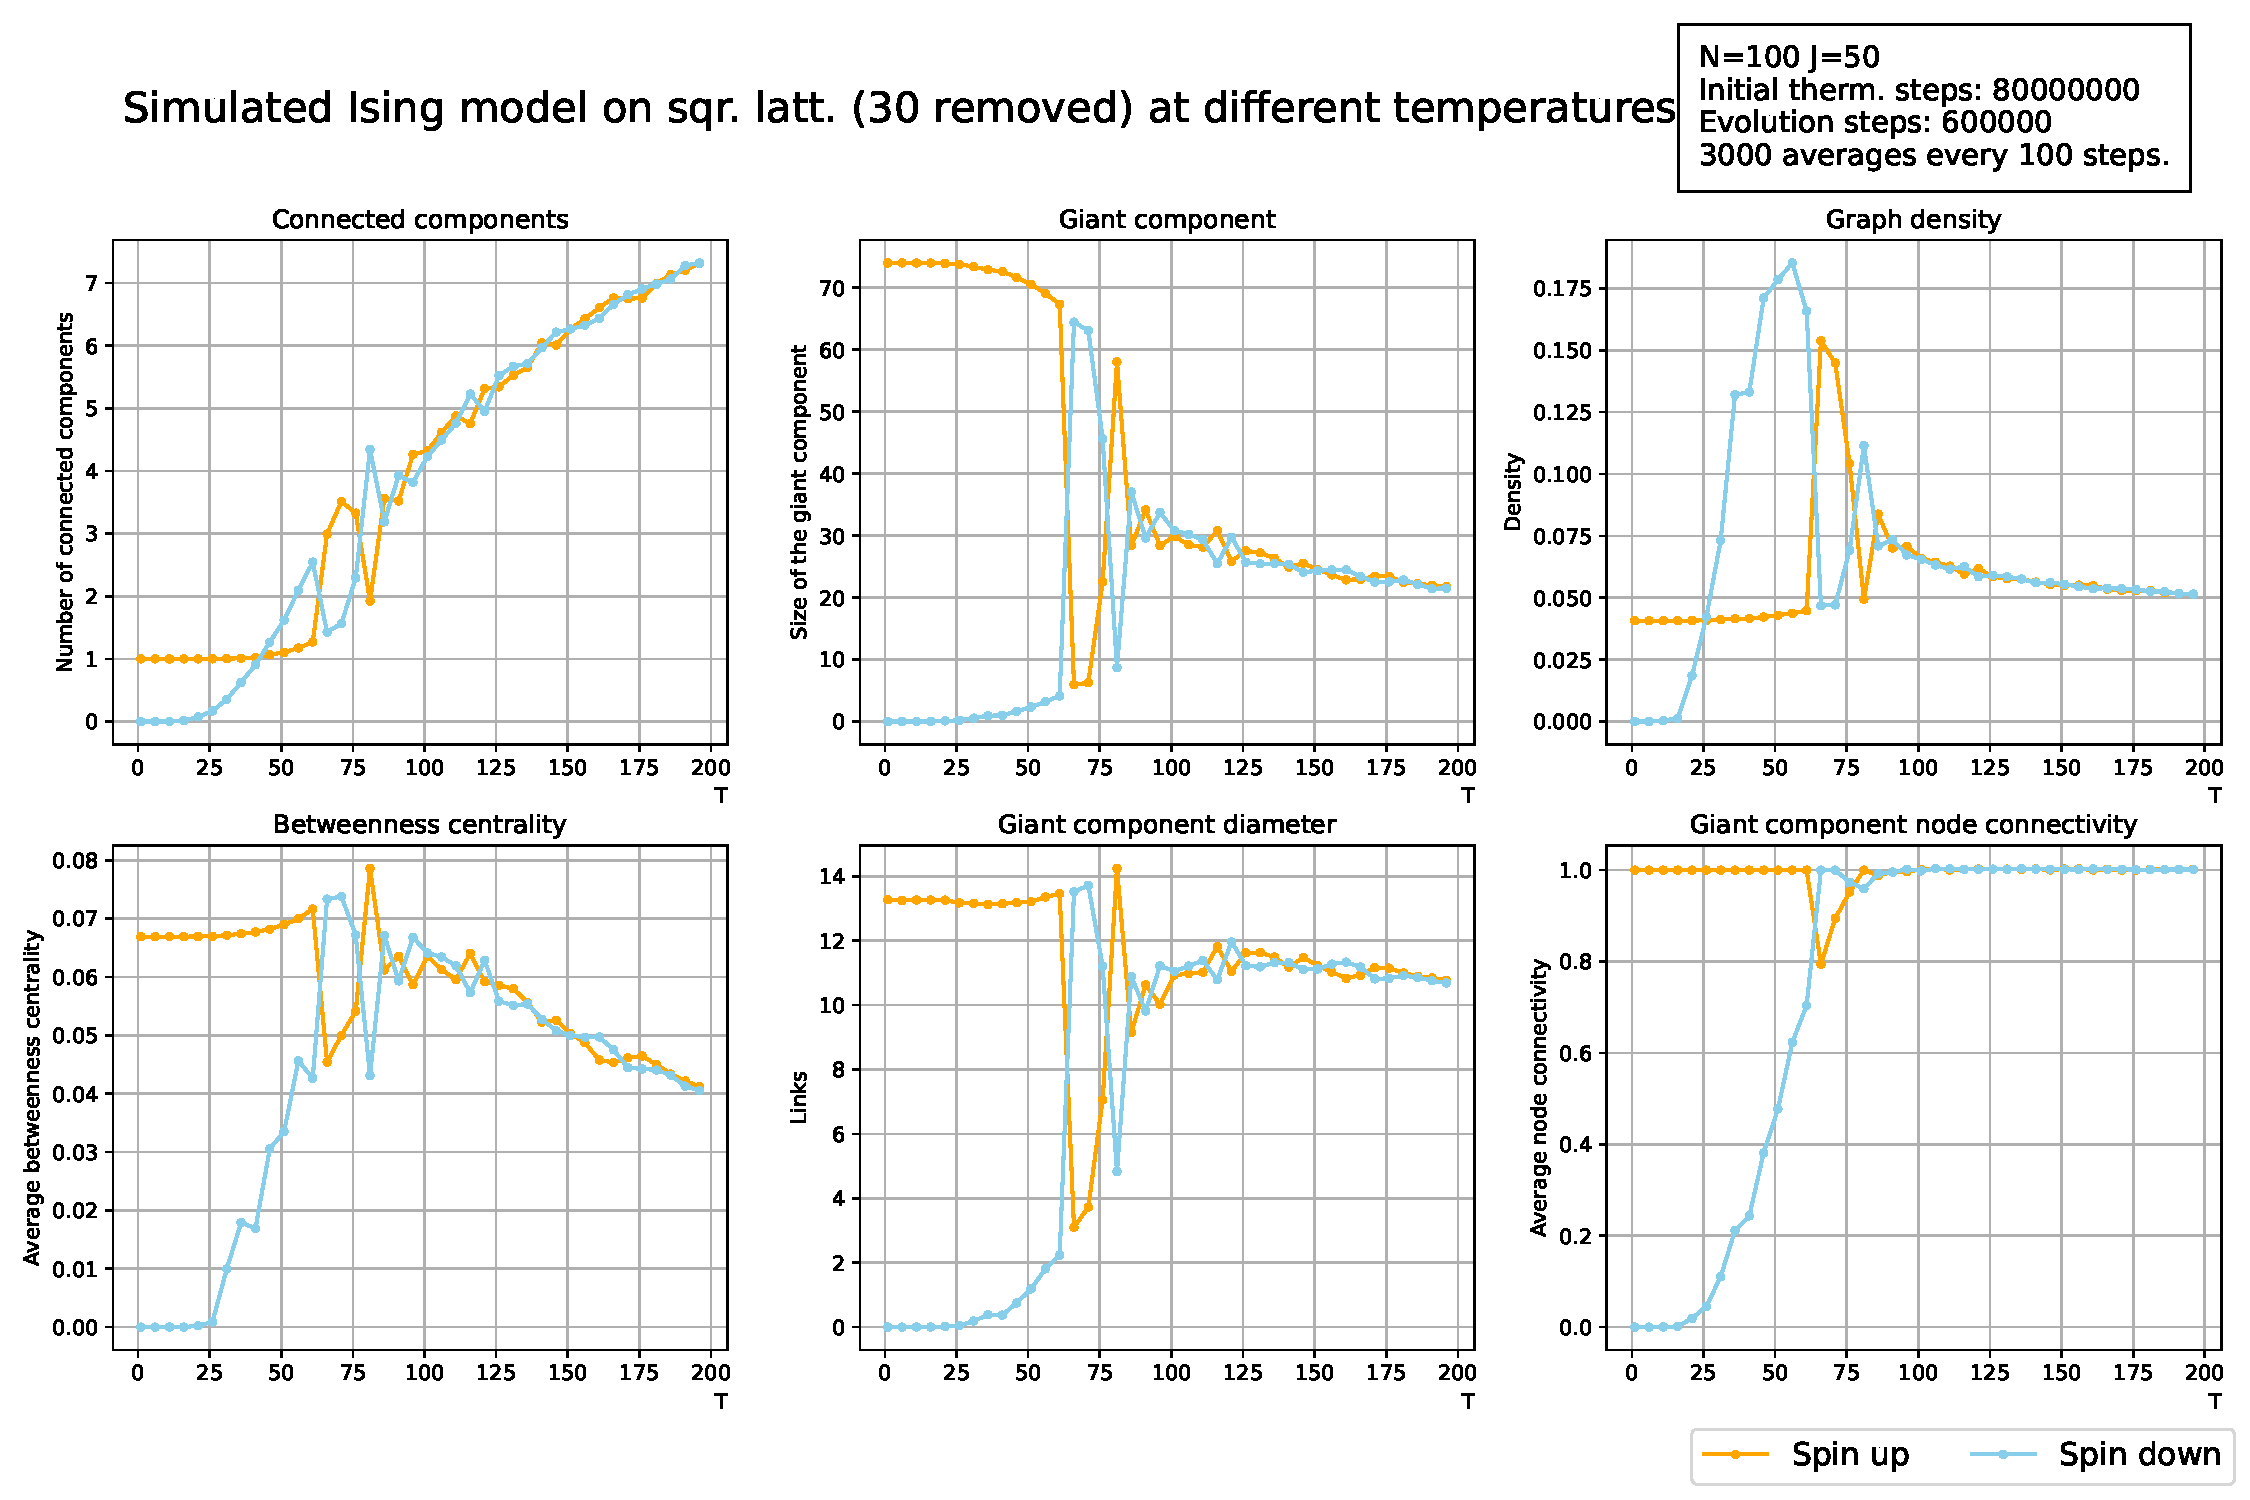
\includegraphics[width=.5\linewidth]{Broken/Square_30.pdf}
    \caption{Behavior of the network proprieties of a square lattice from which we removed 7 atoms. The orange line is the spin up network while the blue is the spin down one.}
    \label{Fig:BSNetworkmeasure}
\end{figure}

\subsubsection*{Herdos-Renyi}
The Herdos-Renyi lattice simulation appears to be different from the other ones: after the phase transition the number of connected components per type of spin increases a little without never showing a clear split in 2 or more components, and also the size of the giant components shows that the lattice is almost perfectly split in two domains. We can also note that the giant component connectivity never drops to 1, as it used in the other lattices. We must conclude that a Herdos-Renyi network is too much connected to generate more tree-like connected components, even though the betweenness centrality still rises after the phase transition. This increment of the betweenness centrality is coherent with the node connectivity, which halves, signaling that the networks becomes less connected but not as much as the previous networks.  
\begin{figure}[!htb]
  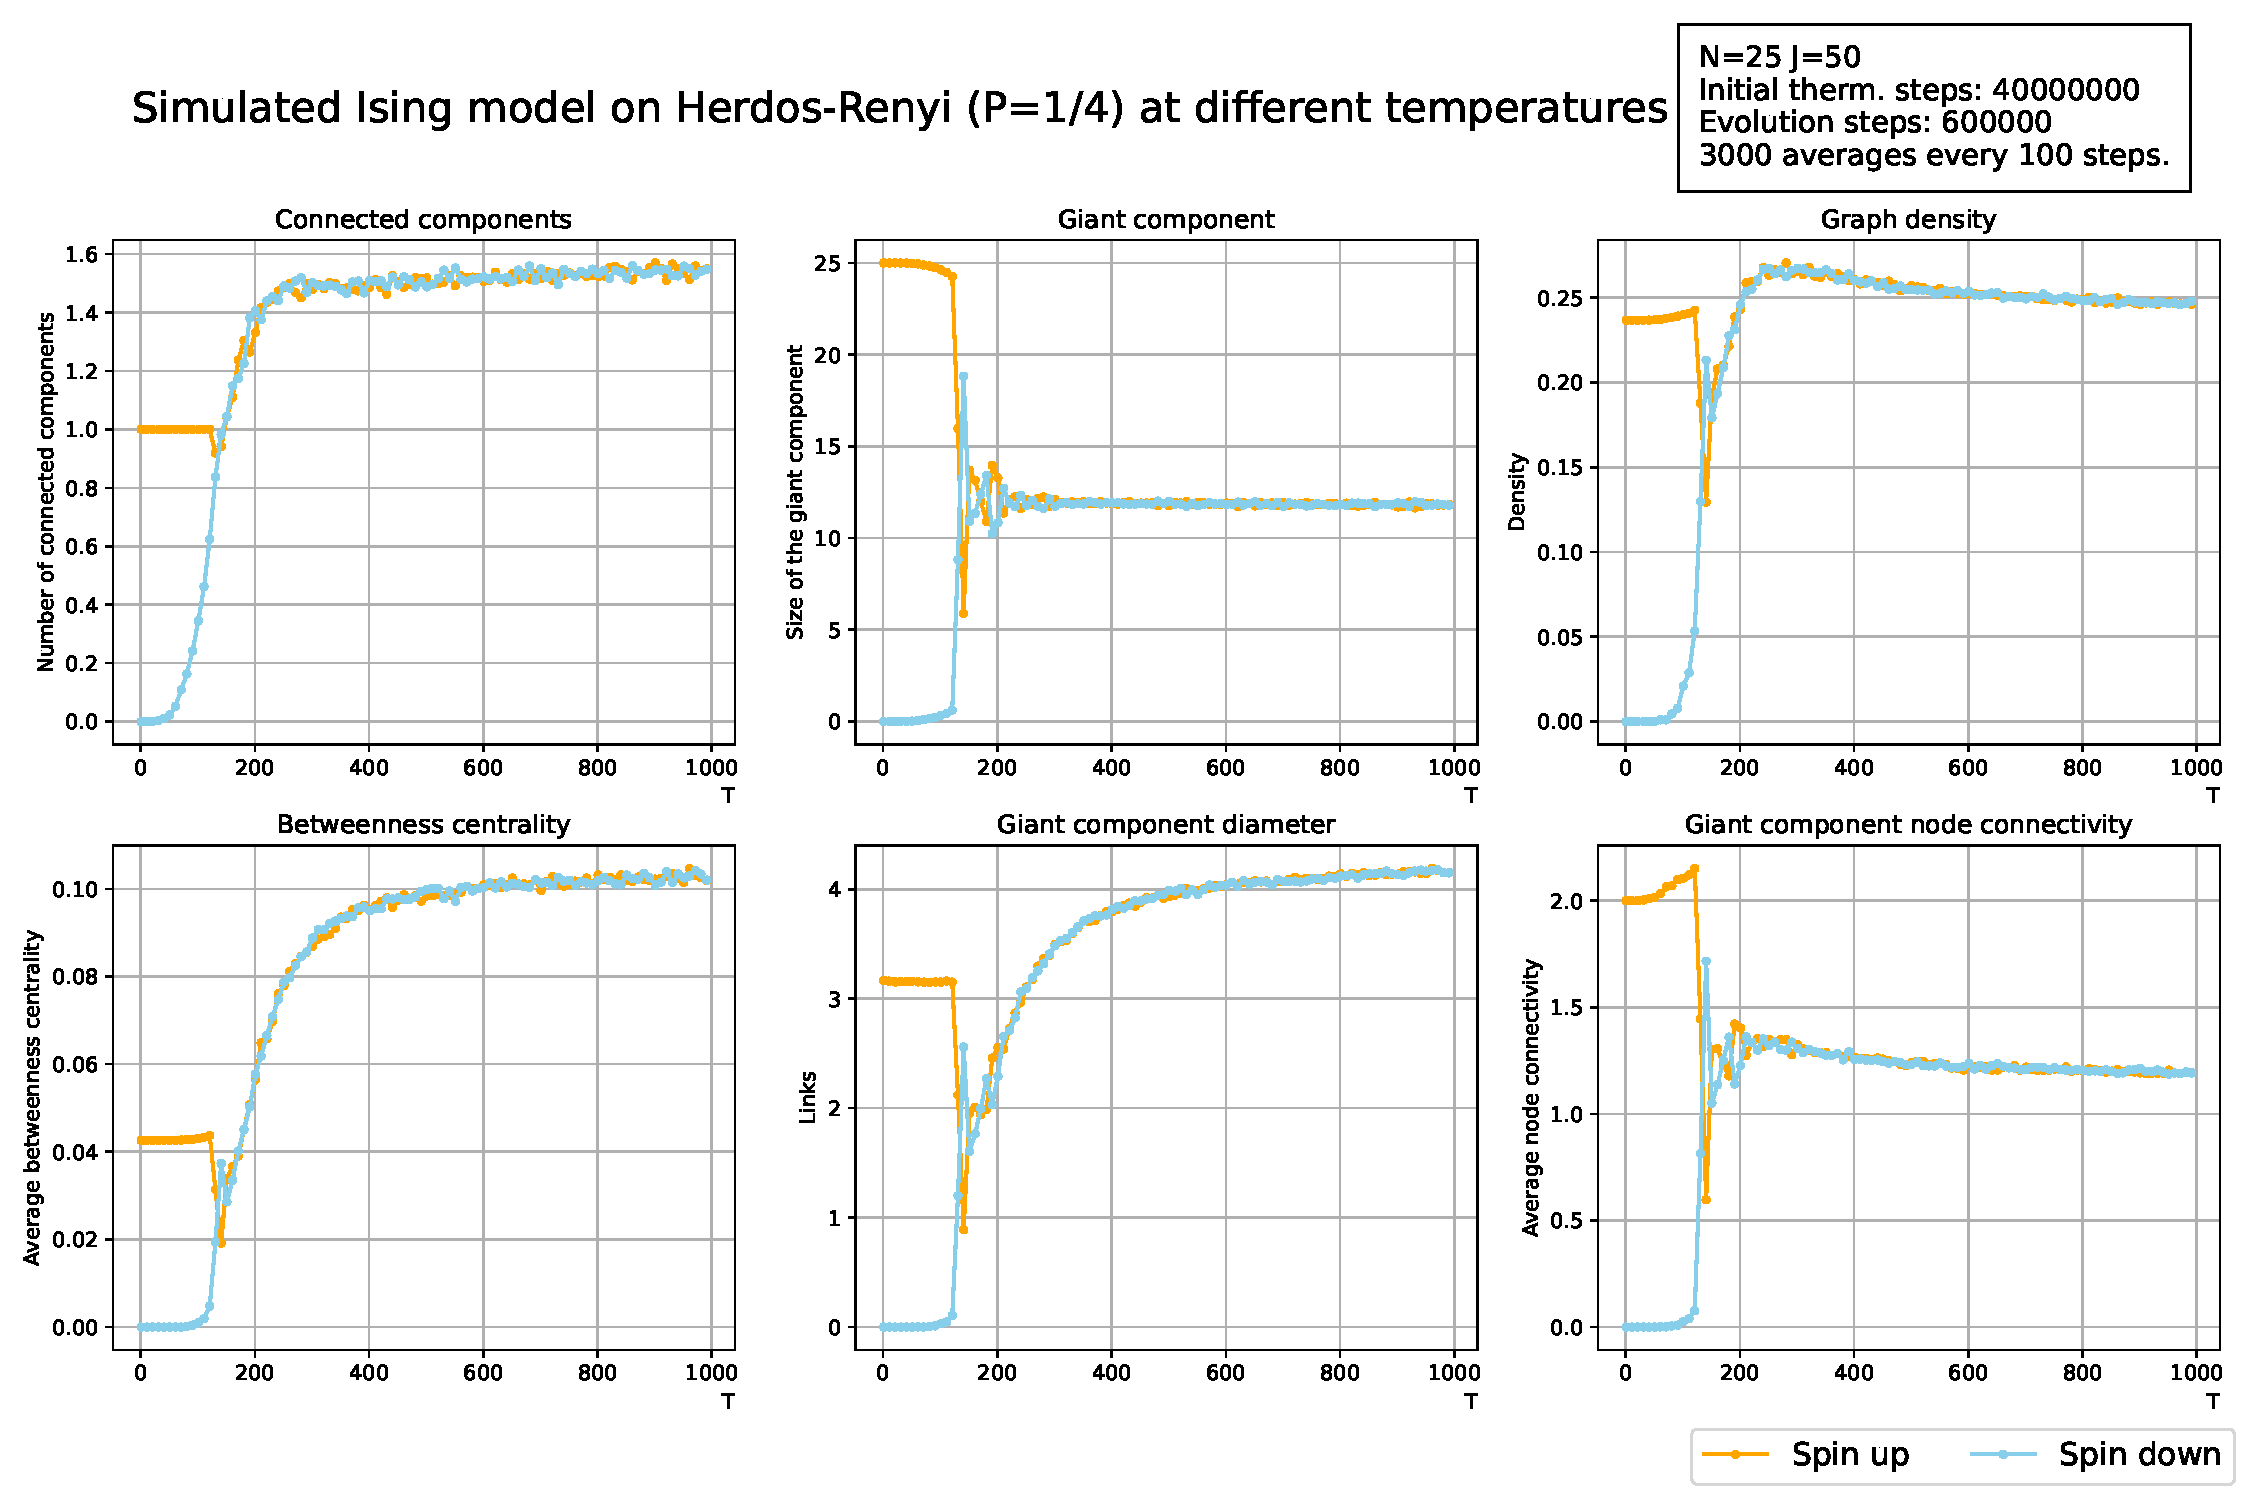
\includegraphics[width=\linewidth]{Network meausres/HR.25_Network.pdf}
    \caption{Behavior of the network proprieties of the Herdos-Renyi lattice at increasing temperatures. The orange line is the spin up network while the blue is the spin down one.}
    \label{Fig:1RHNetworkmeasure}
\end{figure}
Figures \ref{Fig:1RHNetworkmeasure}, \ref{Fig:2RHNetworkmeasure}, \ref{Fig:3RHNetworkmeasure} show different Herdos-Renyi networks with increasing probability of having a link. At lower probability, which produce a graph with fewer edges, the phase transition is still similar to the ones on lattices (Fig. \ref{Fig:1RHNetworkmeasure}), however as we increase the links, by increasing their probability, the features that we already explained become more evident. 

We also noticed that, as we increased the links, the temperatures at which the symmetries of the system are restored starts to shift from the critical temperature that we measure thermodynamically. We can appreciate this shift observing that while transitioning sometimes spin-up and spin-down networks swap: one starts to behave as the other used in a coherent way but losing the information on which one was the original alignment at $T=0$. Meanwhile, the critical temperatures increase as the probability of generating a link increases.
\begin{figure}[!htb]
  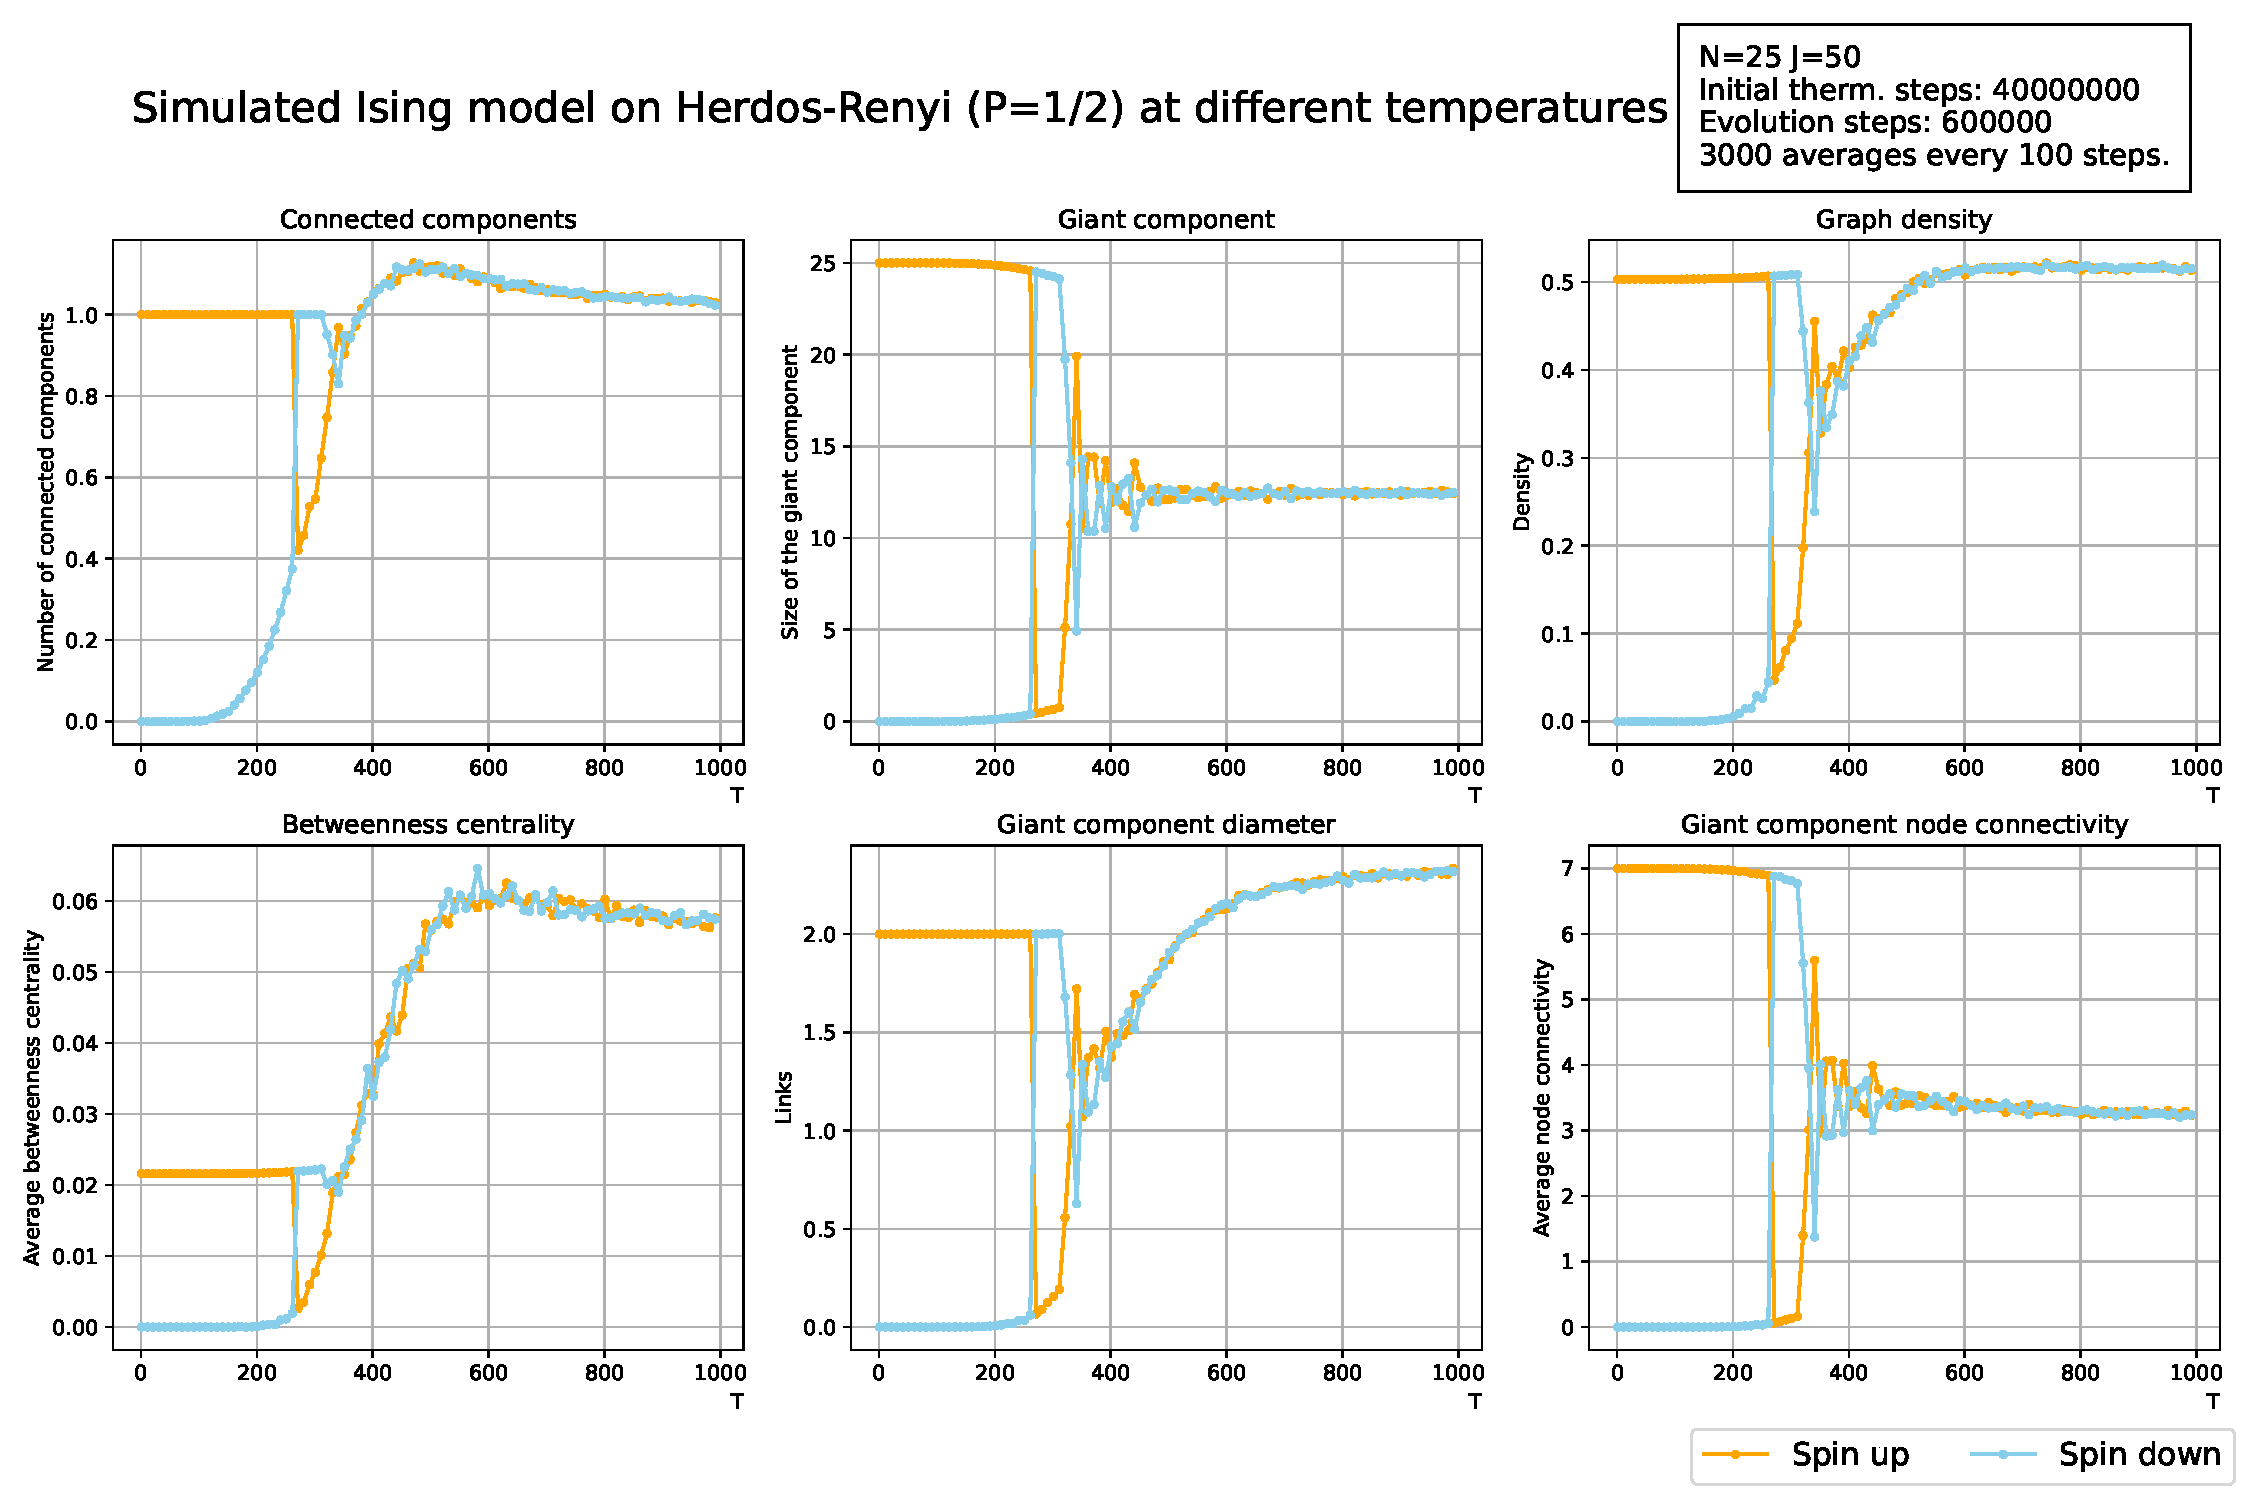
\includegraphics[width=\linewidth]{Network meausres/HR.5_Network.pdf}
    \caption{Behavior of the network proprieties of the Herdos-Renyi lattice at increasing temperatures. The orange line is the spin up network while the blue is the spin down one.}
    \label{Fig:2RHNetworkmeasure}
\end{figure}
\begin{figure}[H]
  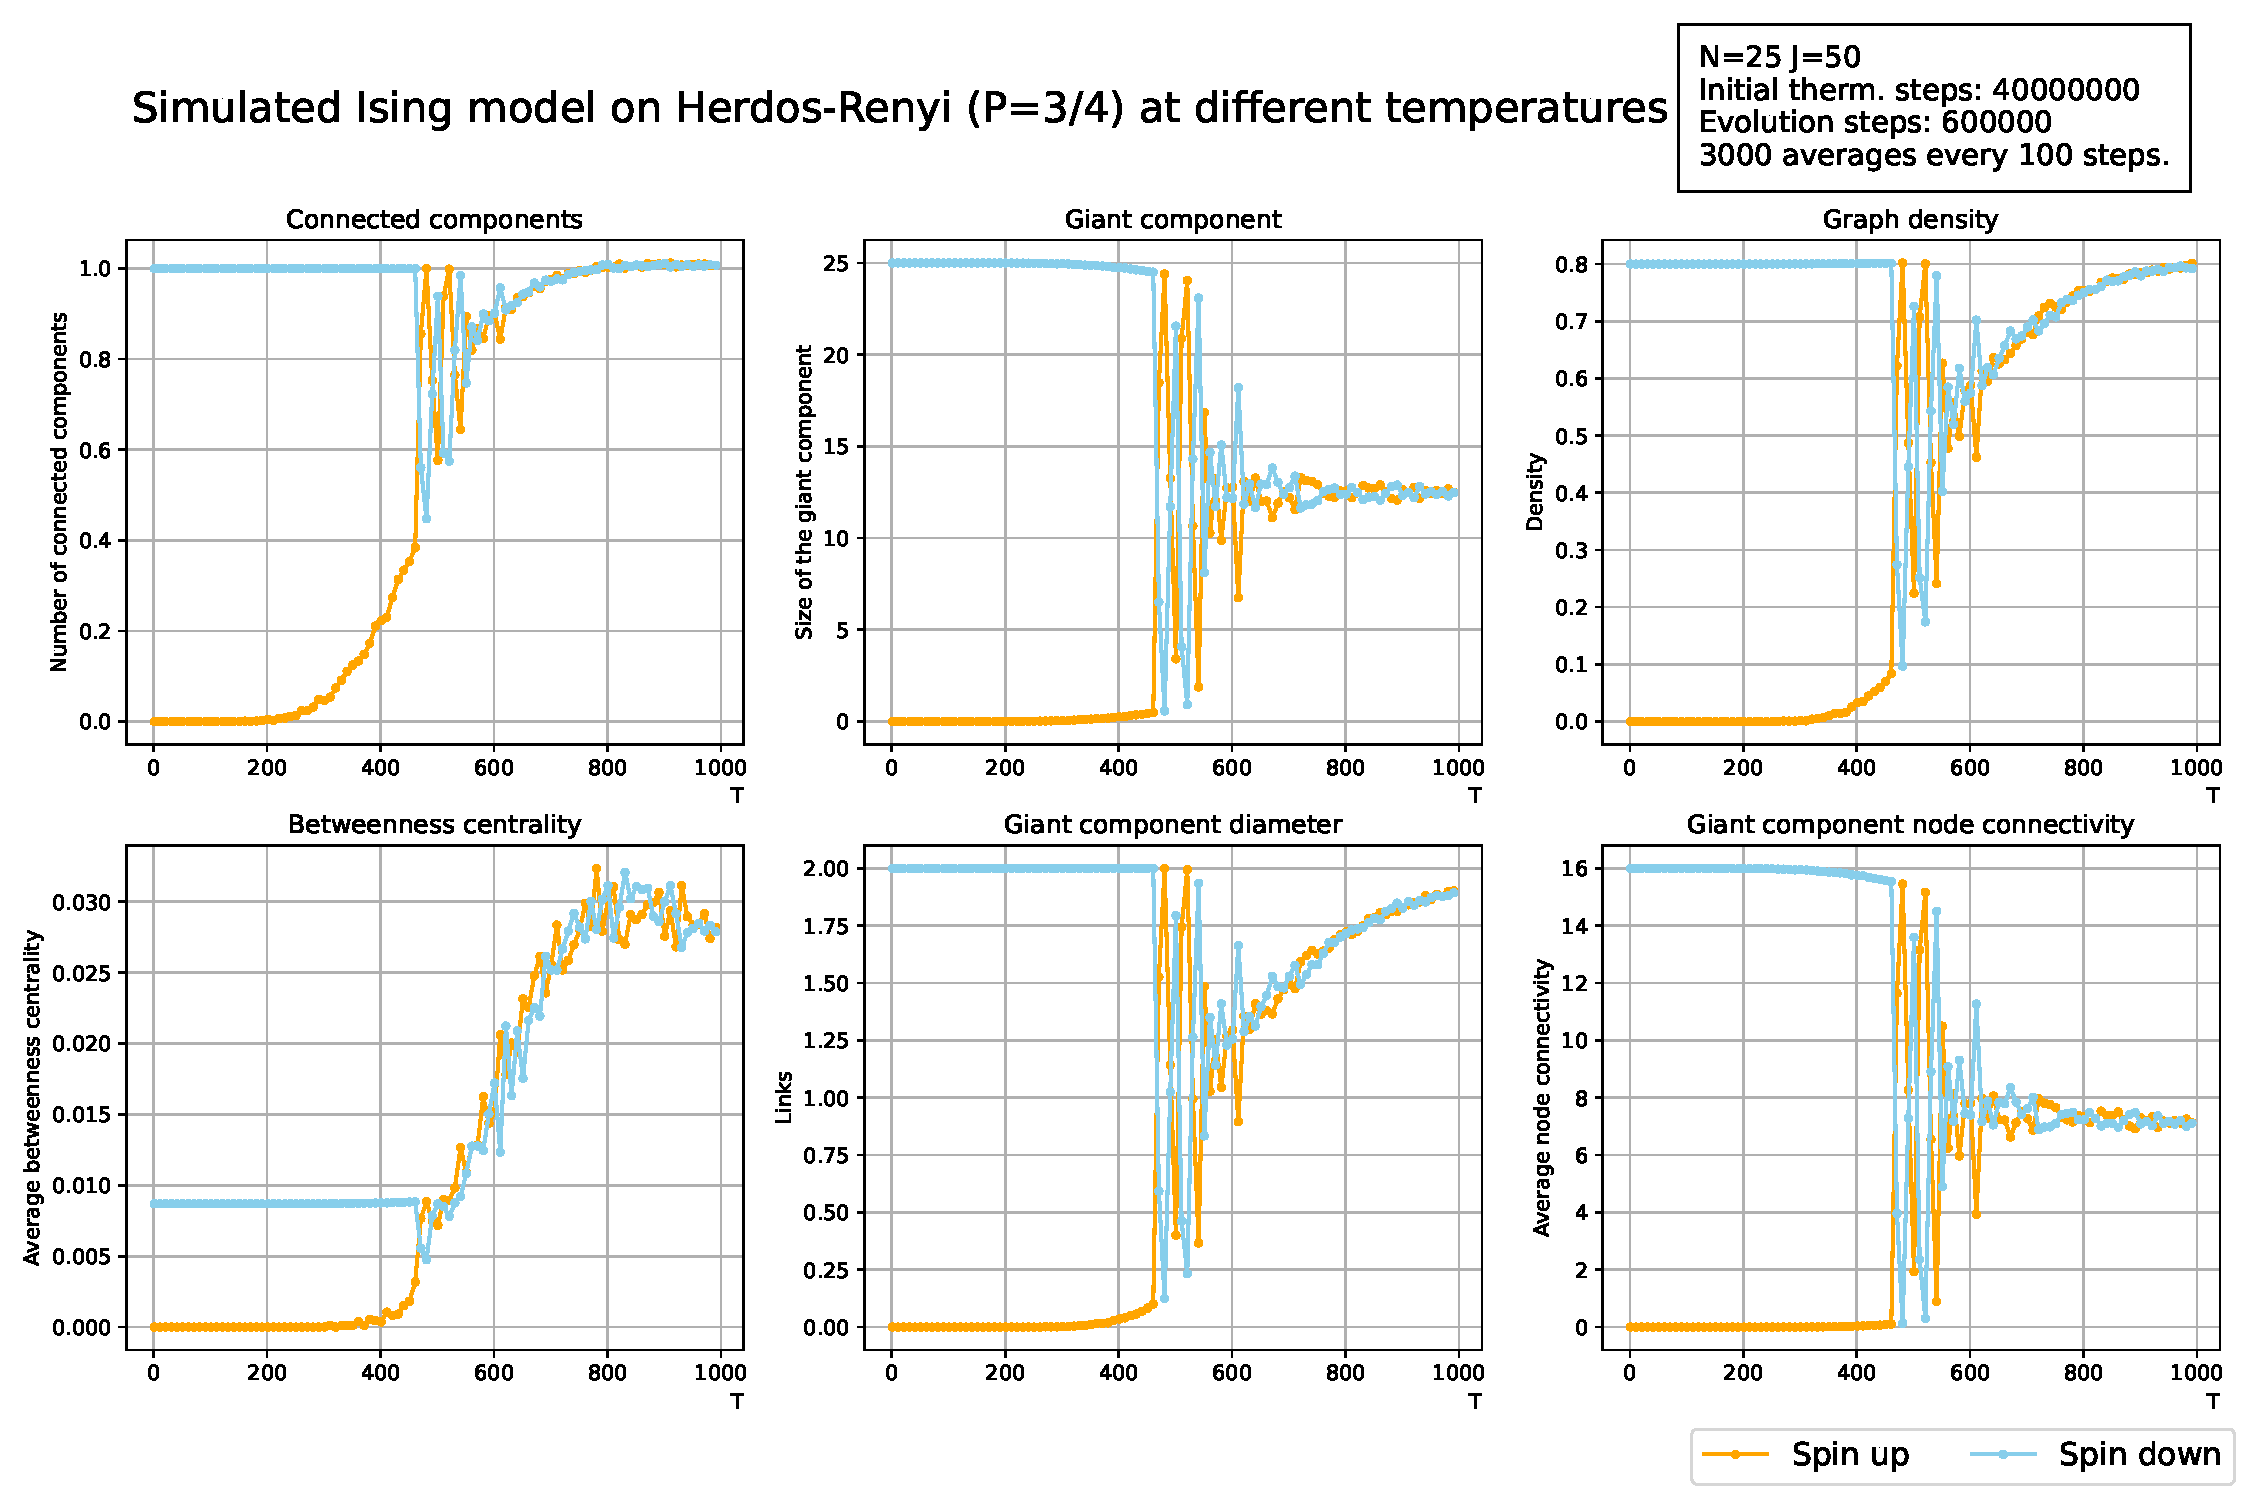
\includegraphics[width=\linewidth]{Network meausres/HR.75_Network.pdf}
    \caption{Behavior of the network proprieties of the Herdos-Renyi lattice at increasing temperatures. The orange line is the spin up network while the blue is the spin down one.}
    \label{Fig:3RHNetworkmeasure}
\end{figure}

\newpage 

\subsubsection*{More than nearest neighbor}
We also simulated the Ising model on lattices where are allowed interactions with the neighbors of the neighbors of each atom. This mimicked short range interactions but over higher distances. We simulated on square, triangular and hexagonal lattices, using parameters comparable  with the one we already used.

Figures \ref{Fig:MNN1}, \ref{Fig:MNN2}, \ref{Fig:MNN3} shows that this longer range interaction showed again a phase transition behavior: in all the lattices we encounter two networks (spins up and spins down) behaving in completely different ways at lower temperatures but becoming completely indistinguishable at higher ones. However, we noticed that these transitions happen at higher temperatures than the normal ones (just nearest neighbors interactions). Furthermore, we noticed that these networks didn't break as much as the regular ones: at higher temperatures they simply divide into two connected components, one of spins up and the other of down.

\begin{figure}[!htb]
  \centering
  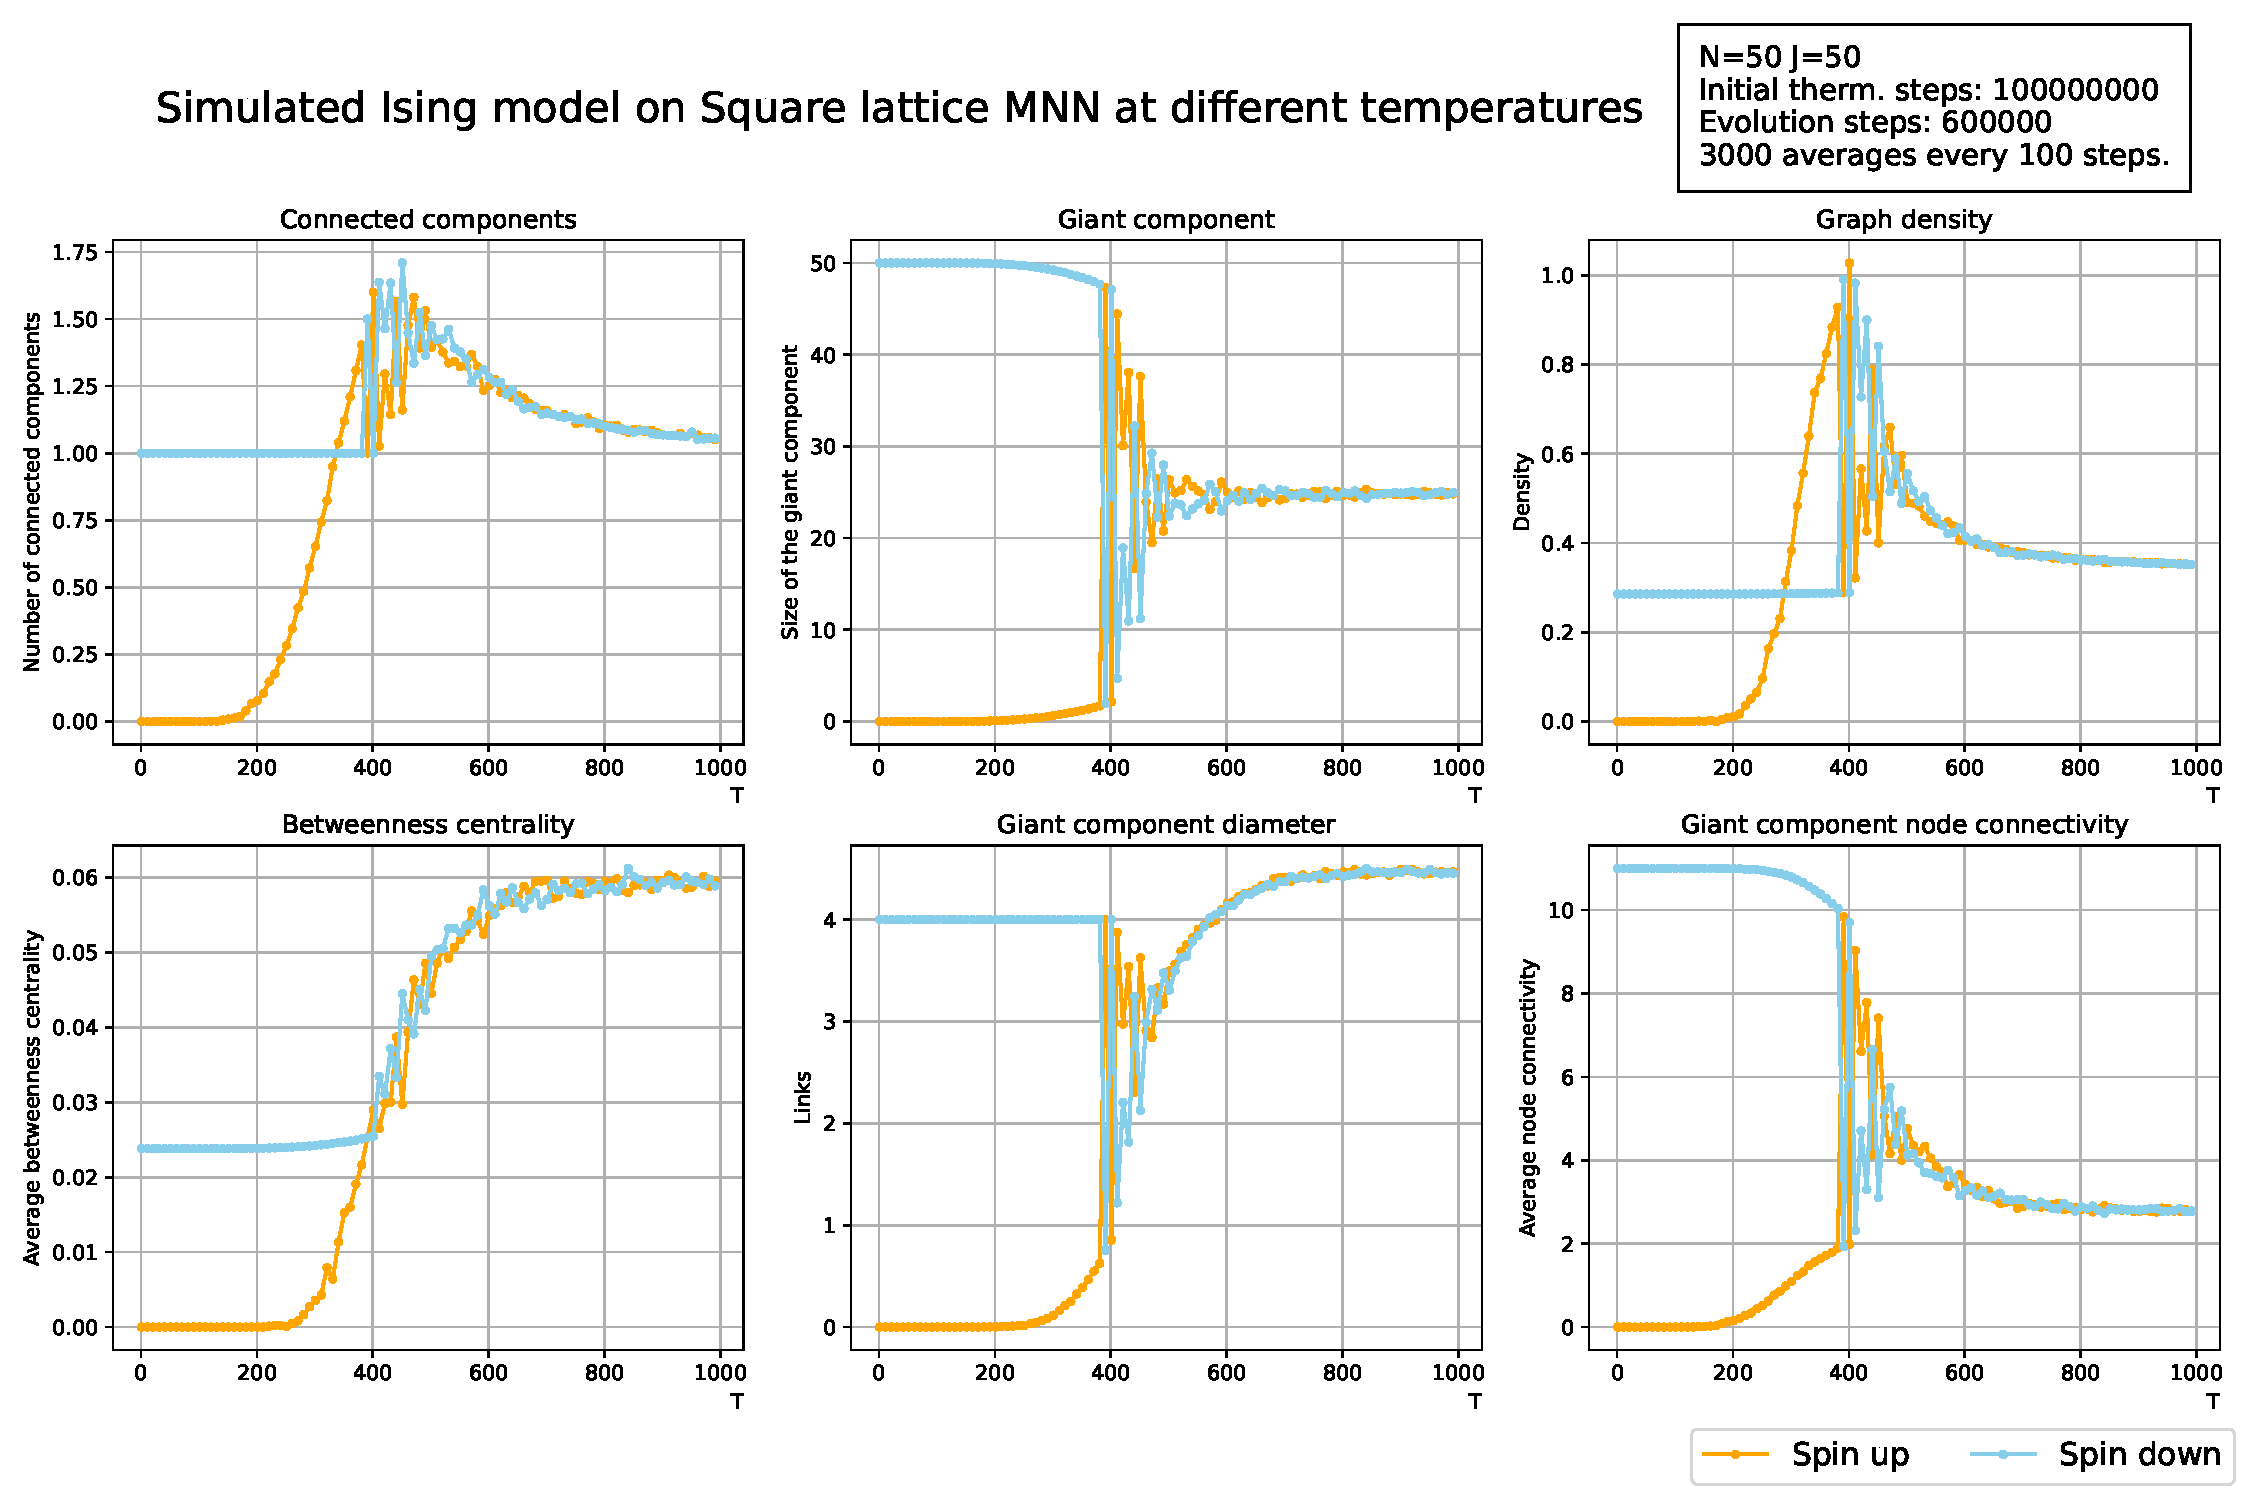
\includegraphics[width=\linewidth]{Network meausres/MNN_Square.pdf}
    \caption{Network proprieties of hexagonal lattice with more than nearest neighbor interactions. The orange line is the spin up network while the blue is the spin down one.}
    \label{Fig:MNN1}
\end{figure}
\begin{figure}[!h]
  \centering
  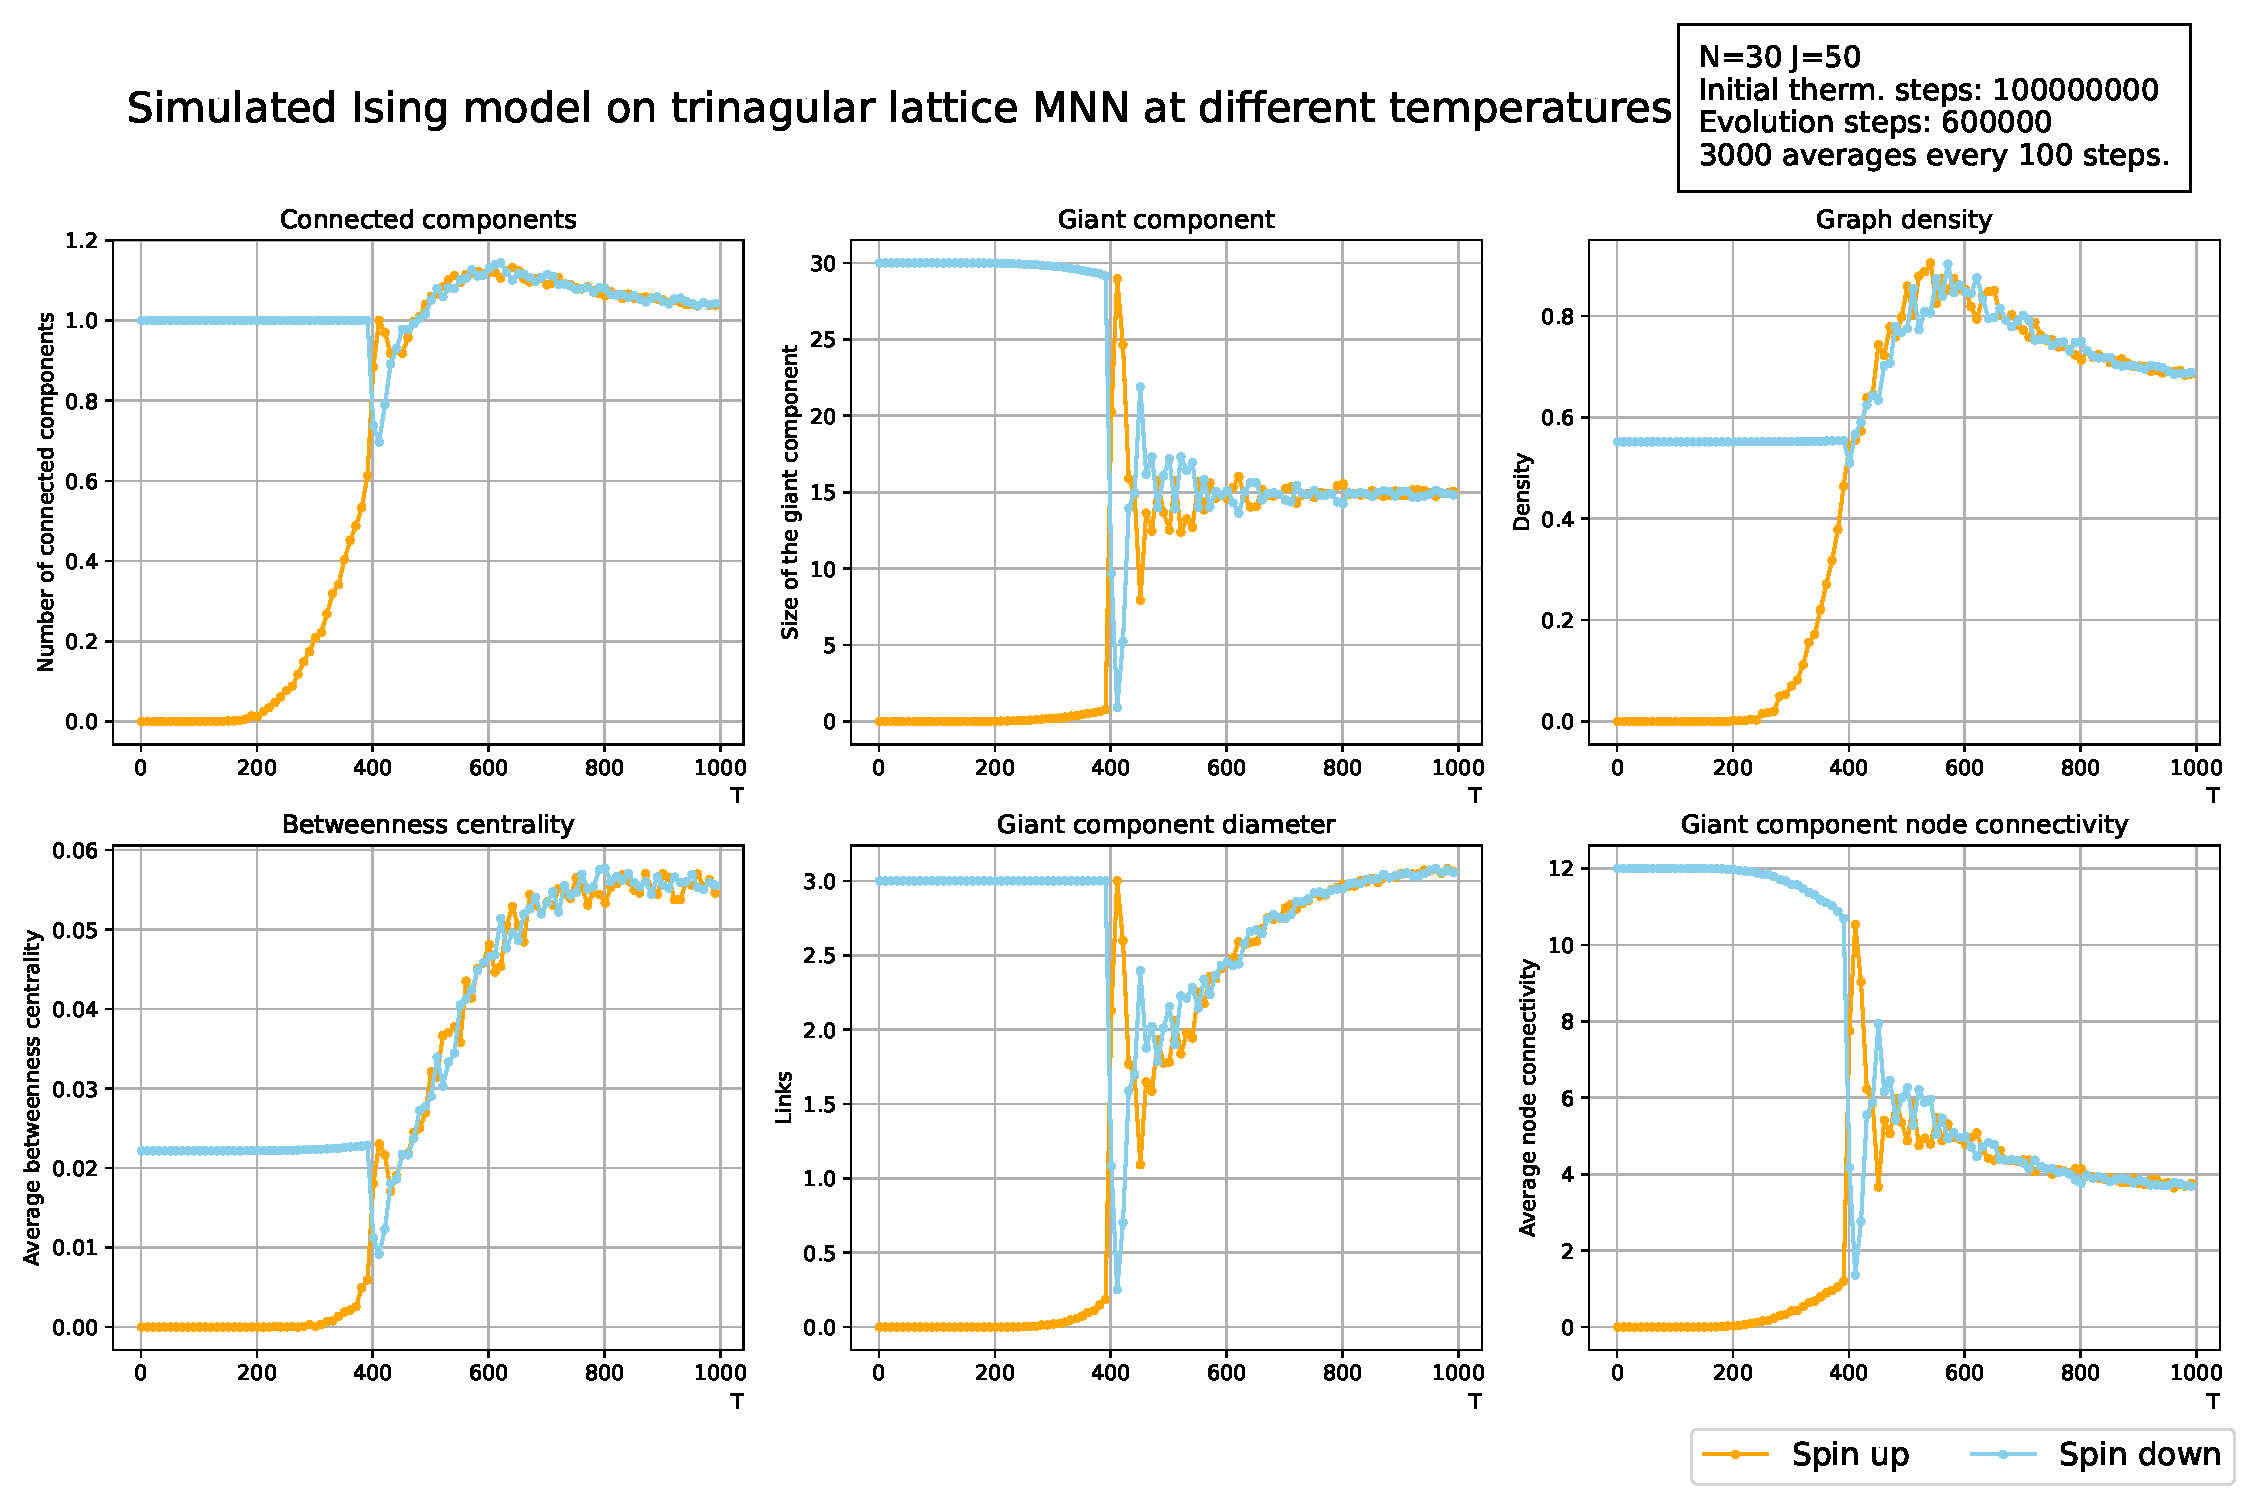
\includegraphics[width=\linewidth]{Network meausres/MNN_Triang.pdf}
    \caption{Network proprieties of hexagonal lattice with more than nearest neighbor interactions. The orange line is the spin up network while the blue is the spin down one.}
    \label{Fig:MNN2}
\end{figure}
\begin{figure}[H]
  \centering
  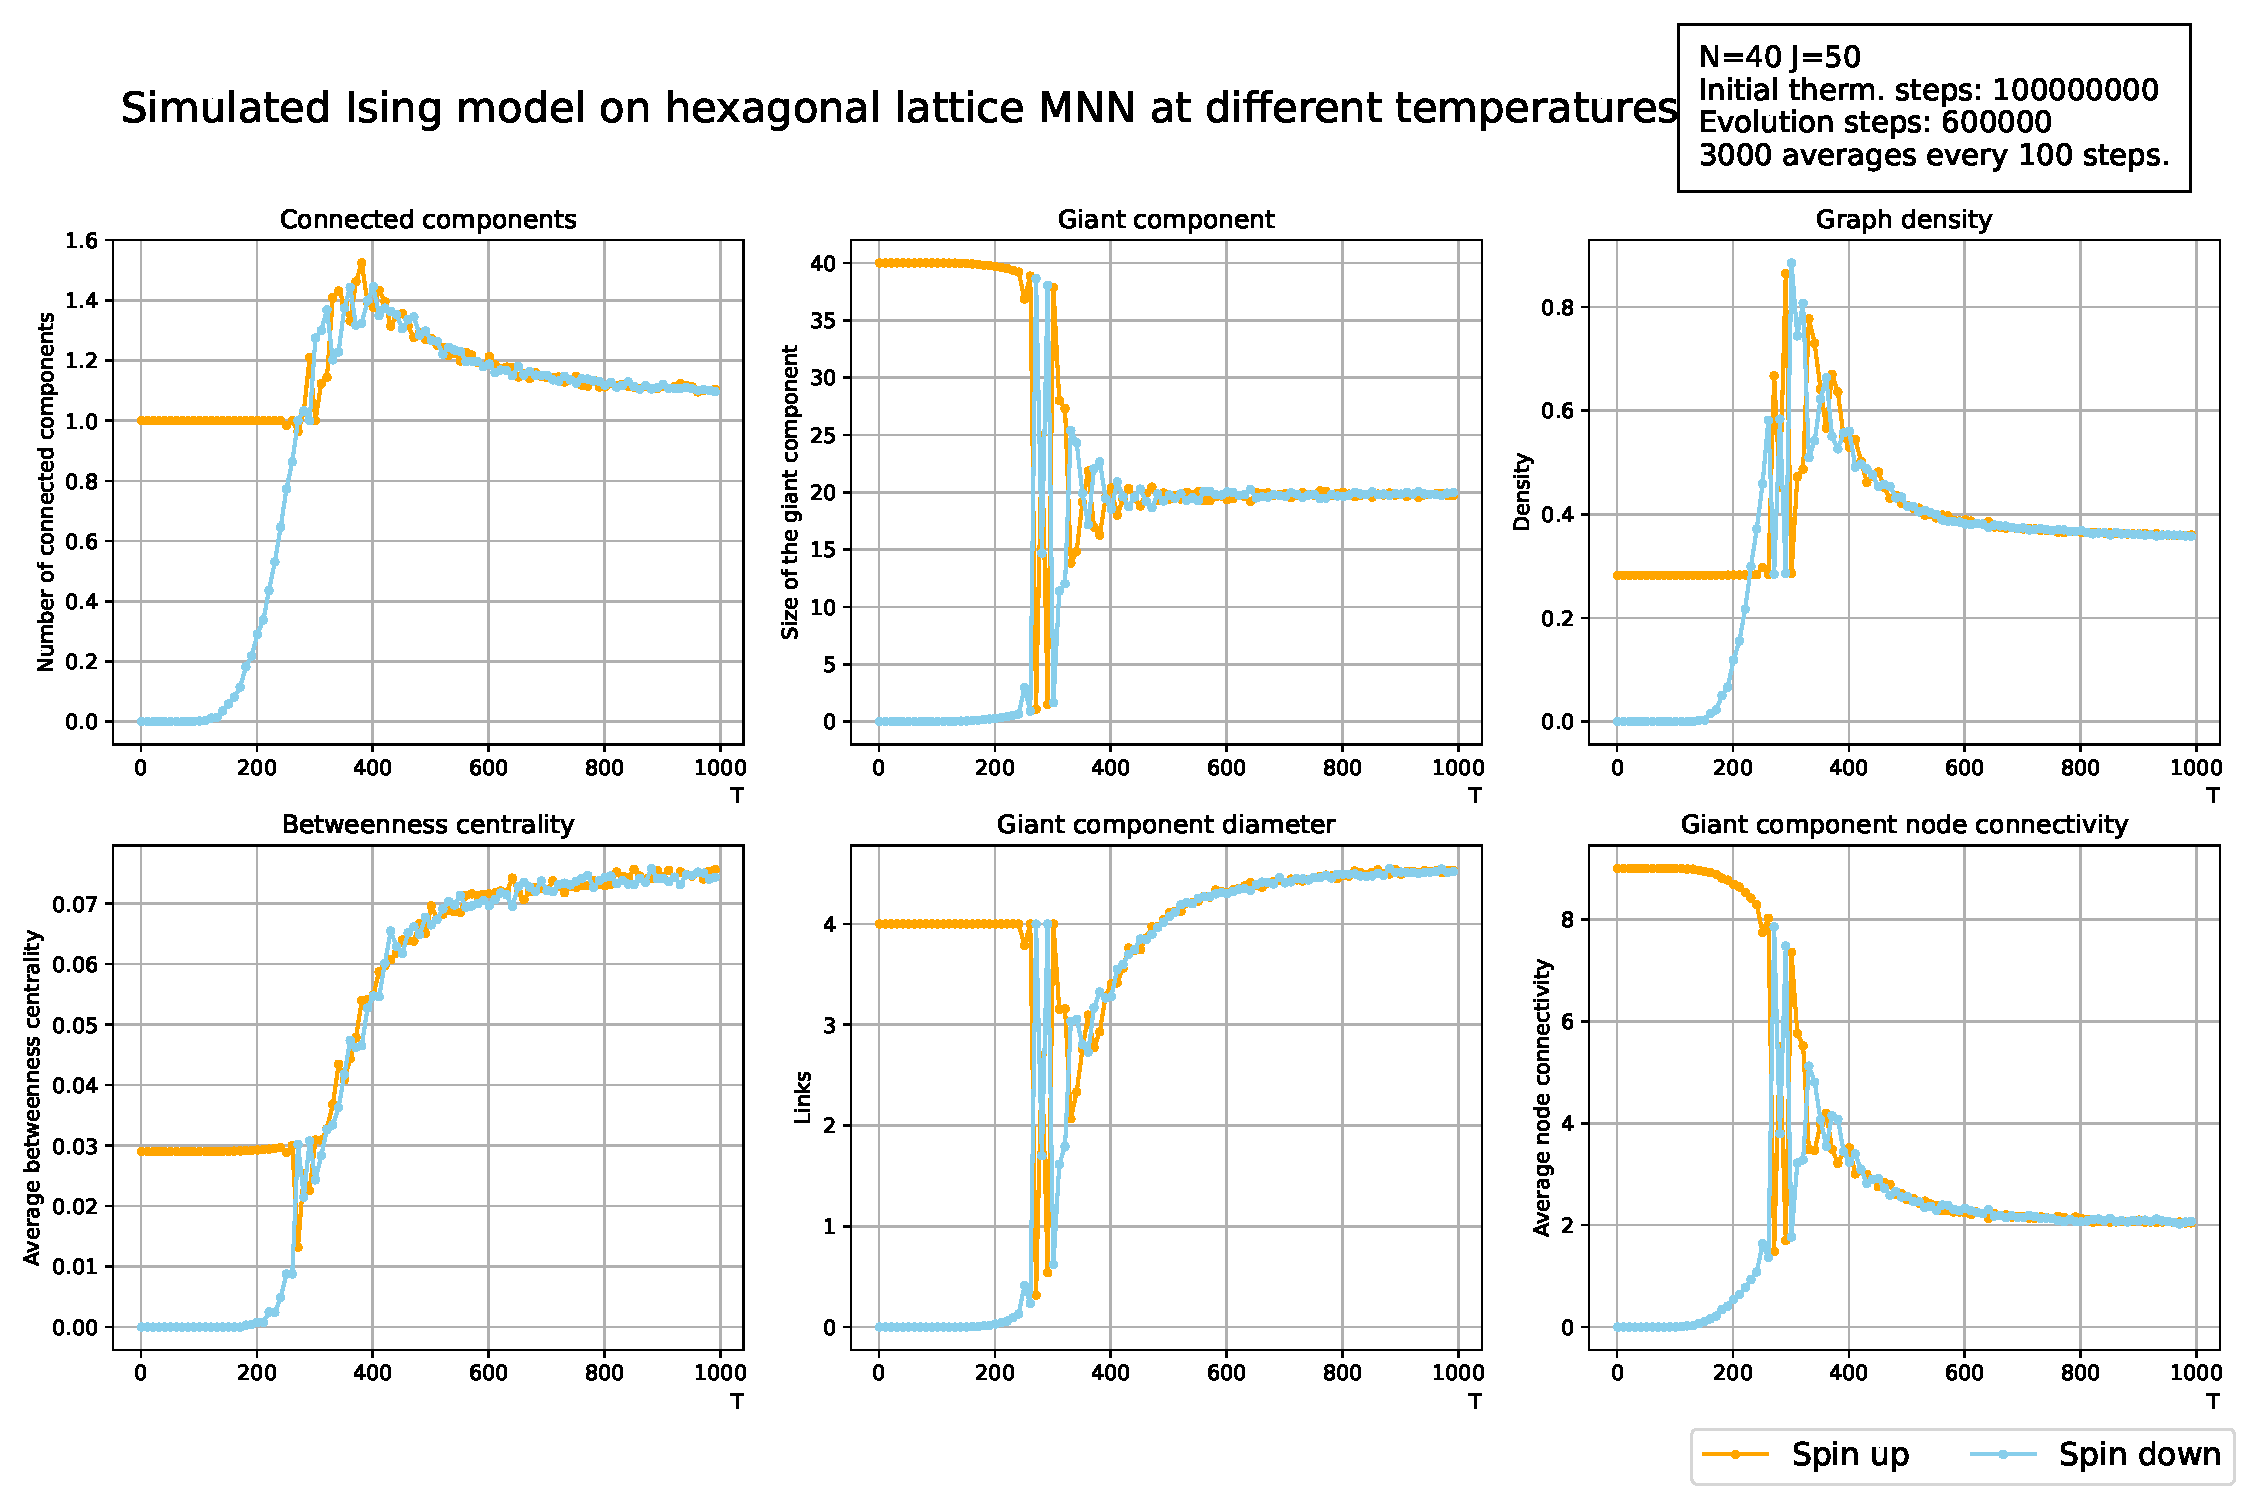
\includegraphics[width=\linewidth]{Network meausres/MNN_Hexa.pdf}
    \caption{Network proprieties of hexagonal lattice with more than nearest neighbor interactions. The orange line is the spin up network while the blue is the spin down one.}
    \label{Fig:MNN3}
\end{figure}
\newpage
\subsubsection*{1-D lattice}
The last simulation we tried is the 1-D lattice. This system is interesting because the exact solution of the Ising model predicts the absence of a phase transition. However, as Figure \ref{Fig:1-D} shows, in our simulation occurred a phase transition at low temperature in both circular graphs (closed loops) and open chains. This is probably due to the small number of atoms that we used.
\begin{figure}[H]
  \centering
  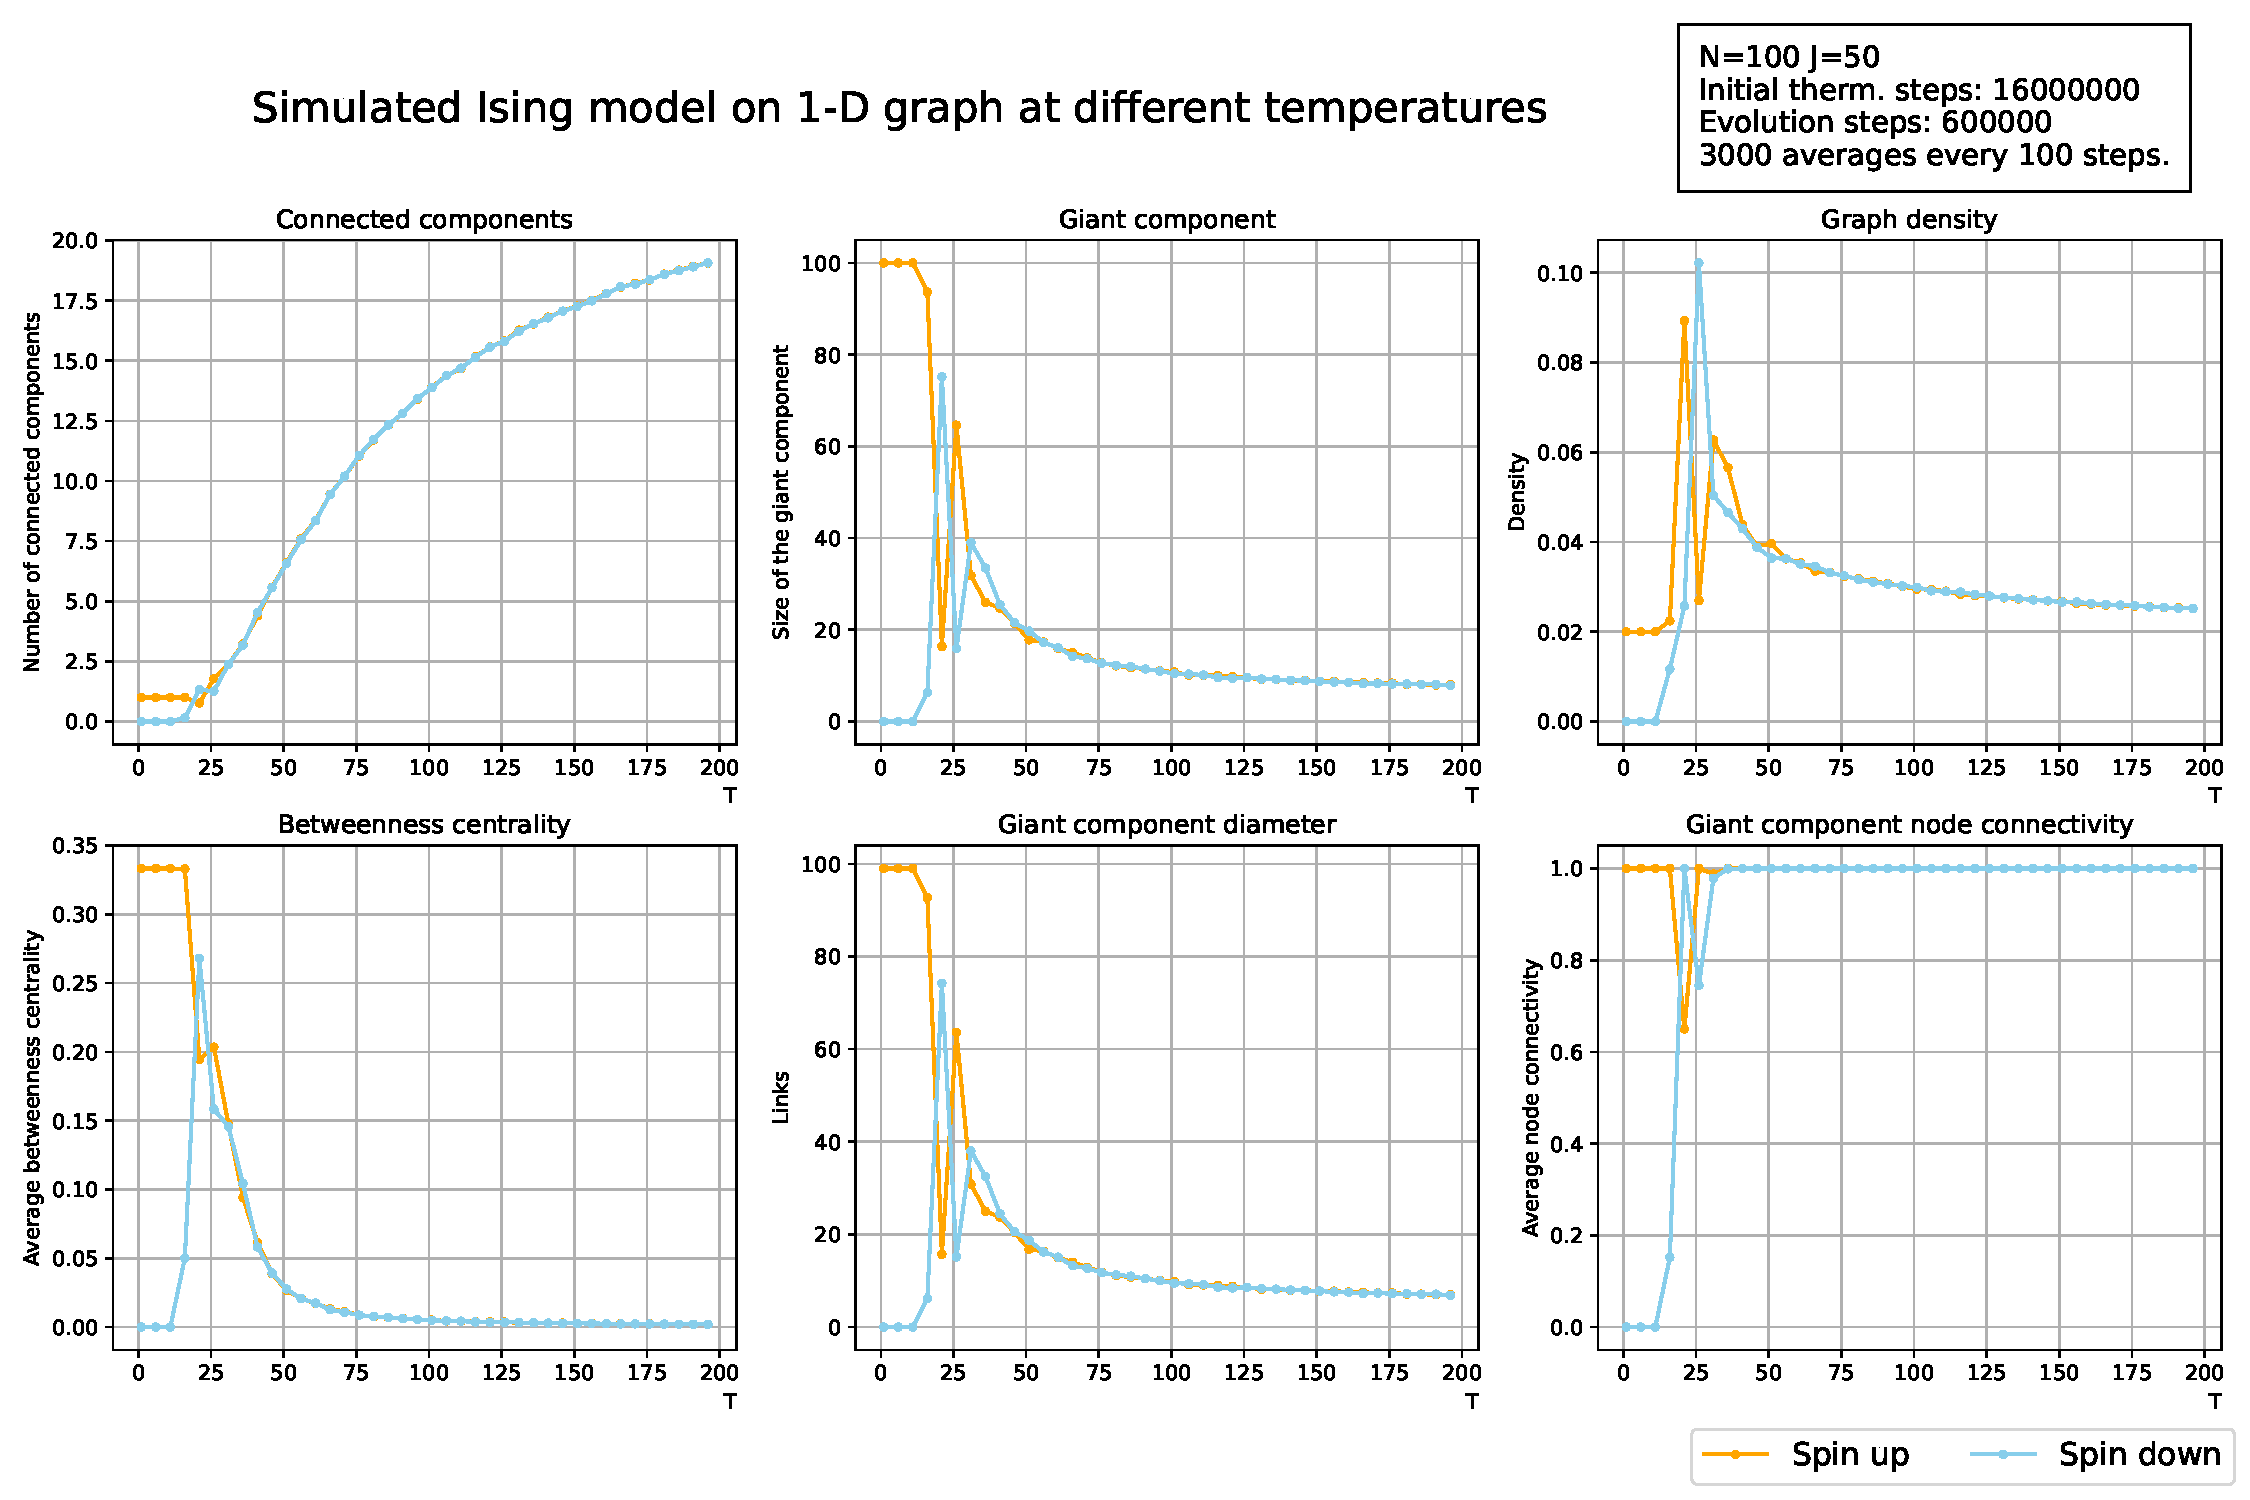
\includegraphics[width=.9\linewidth]{Network meausres/1-D100.pdf}
  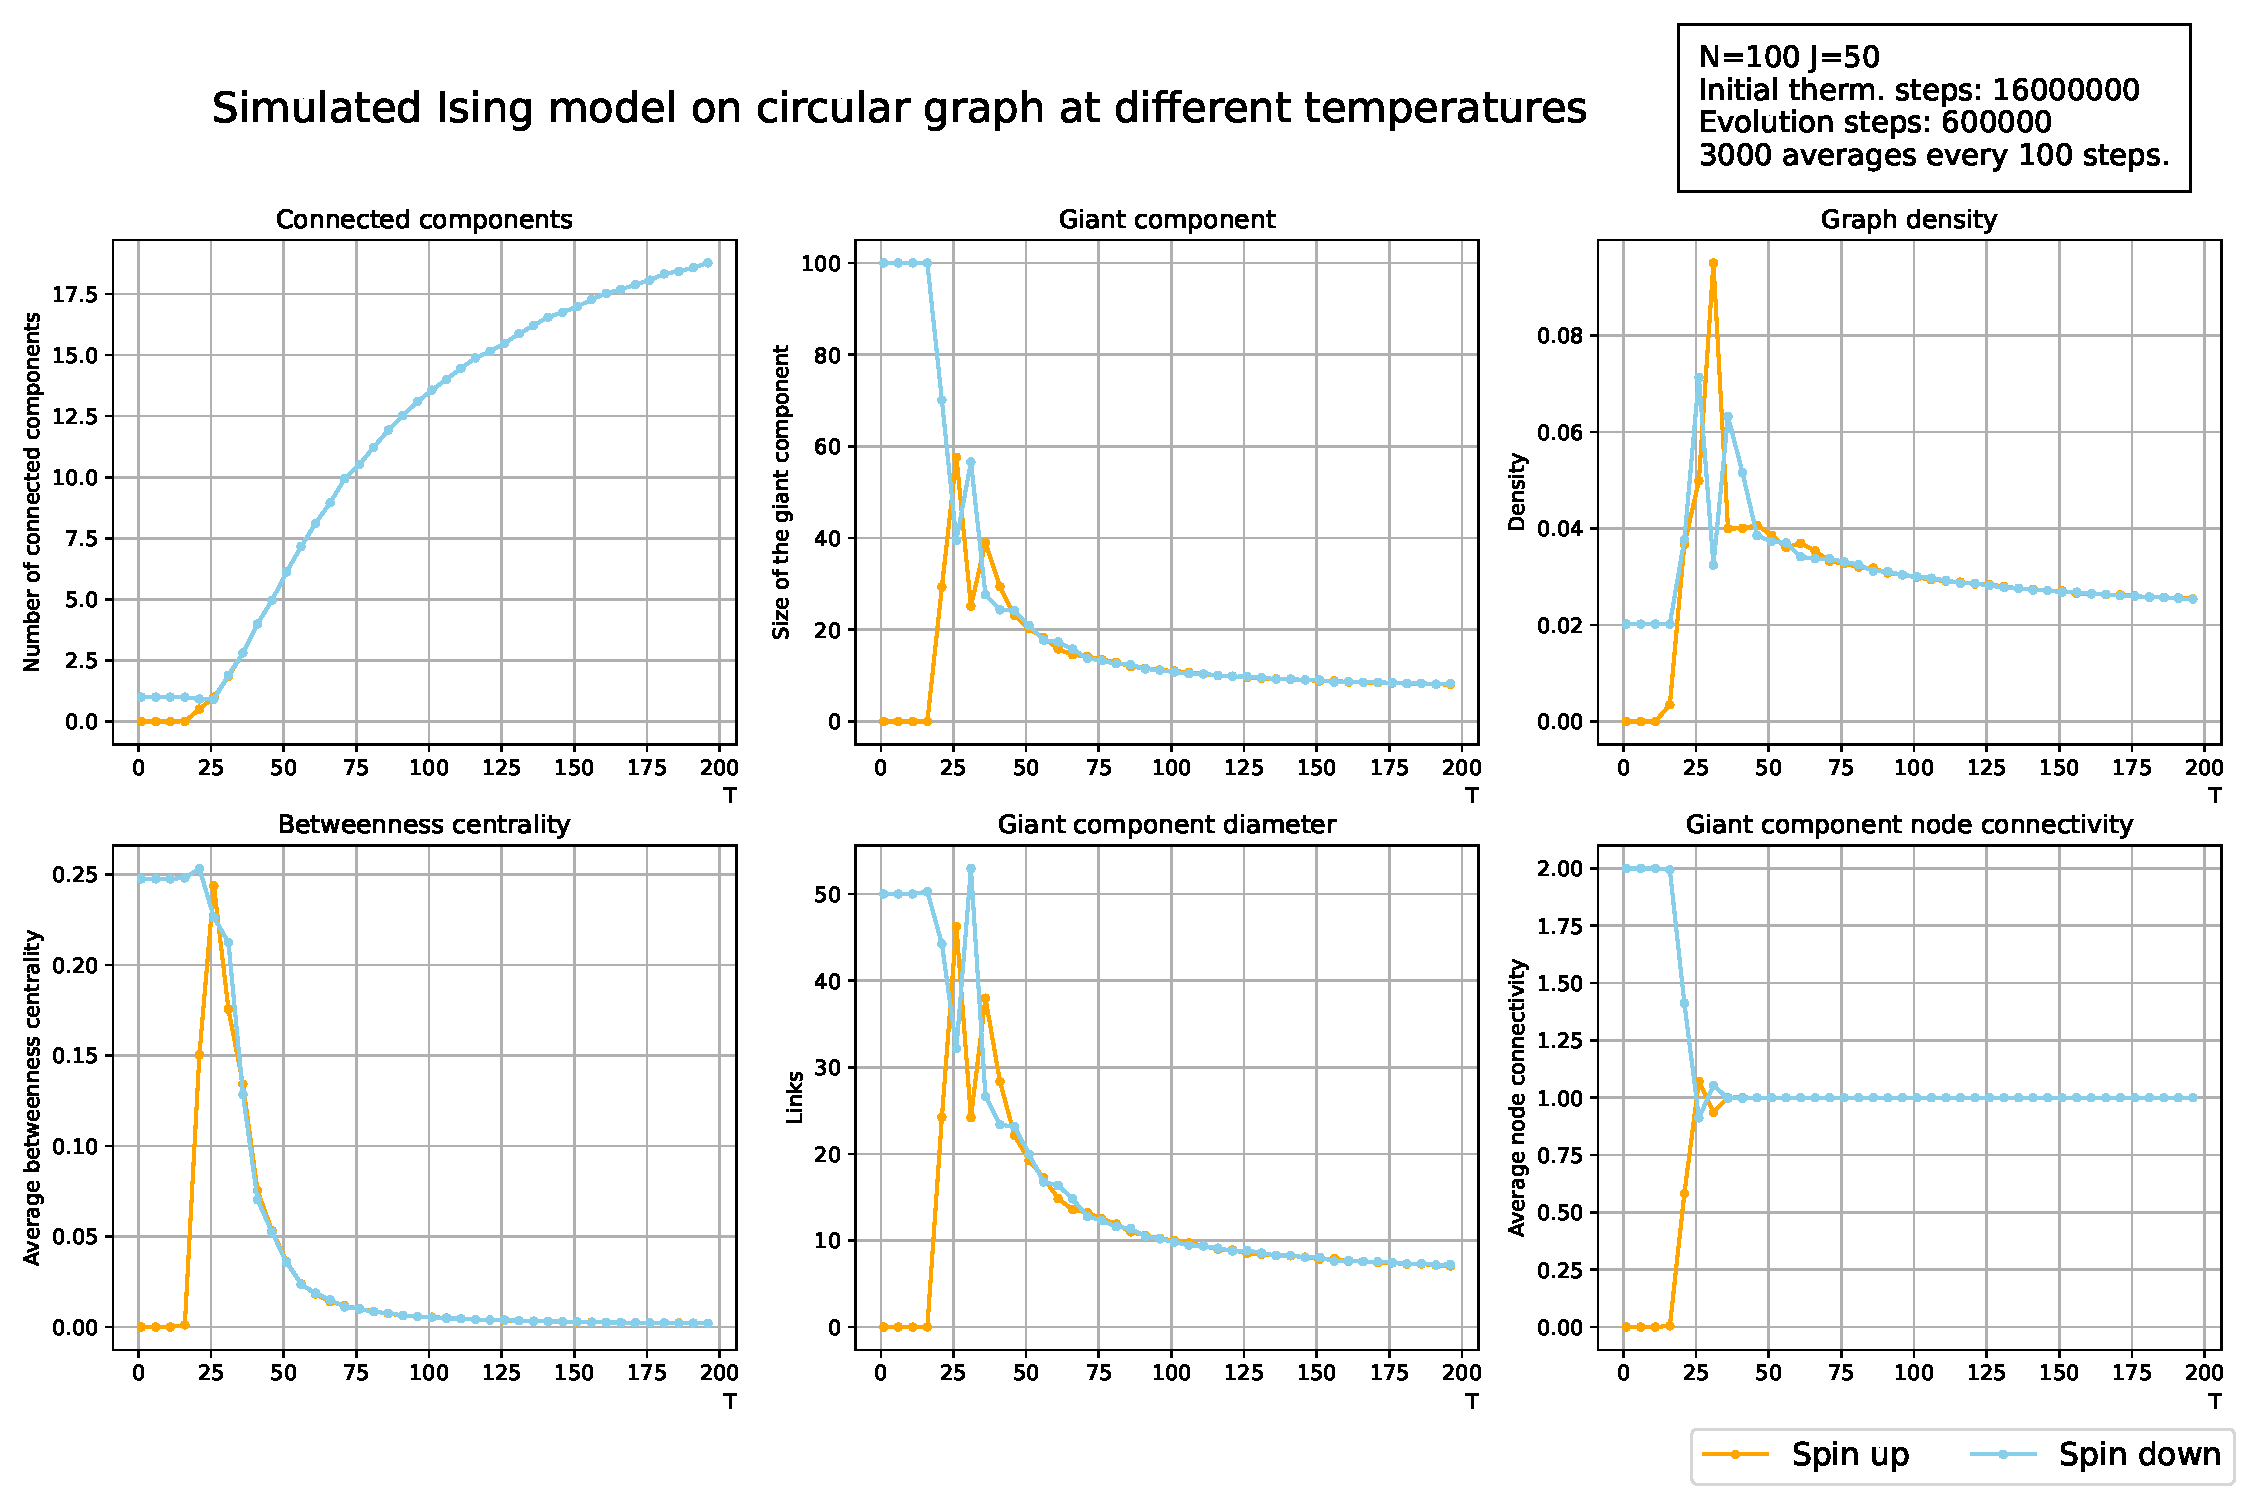
\includegraphics[width=.9\linewidth]{Network meausres/Circular100.pdf}
    \caption{Behavior of the network proprieties of a 1-D lattice and a circular graph at increasing temperatures. The orange line is the spin up network while the blue is the spin down one.}
    \label{Fig:1-D}
\end{figure}

\section{Conclusions}
In this project we simulated the Ising model on different networks. Then, measuring the proprieties of the networks generated by neighbors aligned atoms, we studied the behavior of the system in different temperatures.

First, we compared the critical temperatures, measured using the specific heat and the magnetic susceptibility, with the theoretical ones for the 2-D square, triangular and hexagonal lattices. All these measures showed agreement between the simulations ($T_{CV}^{Sq}=1.11\times10^2,\ T_{\chi}^{Sq}=1.13\times10^2,\ T_{CV}^{Tri}=1.78\times10^2,\ T_{\chi}^{Tri}=1.77\times10^2,\ T_{CV}^{Hex}=6.1\times10^1,\ T_{\chi}^{Hex}=6.6\times10^1$) and the exact solutions ($T^{Sq}= 1.134645\times 10^2,\ T^{Tri}= 1.82048\times 10^2,\ T^{Hex}=7.5\times 10^1$). Measurements of the magnetization showed the phase transition behavior expected in all the simulations and also the entropy, the energy and the free energy behaved in the expected way.

We also measured from all the previous networks some network quantities: this was done by splitting each network into spin up and down networks, in order to obtain graphs describing how aligned atoms group together in the lattice. These measures showed the phase transition also from the network perspective highlighting the spontaneous symmetry breaking of the system: in fact the two networks behave in totally different ways before and during the phase transition, but then they become indistinguishable. We were also able to study the fragmentation of the different lattices after the phase transition: all networks, from a single giant component, broke into to big components (one of spin up and the other of spin down) with a few satellites. The bigger ones showed a bigger diameter and a smaller connectivity, signaling that at high temperatures aligned spins are more disperse. Also, the betweenness centrality showed a rise after the phase transition in accordance to our previous considerations. We also noticed that for all lattices the connectivity always dropped to approximately 1, indicating that aligned spins group together in tree-like networks.

Lastly, we studied other networks. We tried to break the square lattices by removing some atoms in order to mimic defects of the lattices. This first analysis showed that as we removed more atoms the lattices broke in more and more connected networks of aligned spins. We also observed that the time required for the thermalization of the system increased too. The second type of network analyzed is the Erdős Renyl one: our simulations showed that this network, that could be interpreted as a system with random long and short range interactions, still posses the same phase transition behavior, however at high temperatures we get more connected networks of neighbor aligned spins. We also tried to simulate lattices in which each atom can interact with the neighbors of its neighbors: in this case we observed phase transitions at higher temperature and with only one connected component for spin type at high temperatures.  Lastly, we simulated 1D lattices (in closed loops and not) and unexpectedly we still observed a phase transition.

We can conclude that the direct measure of the proprieties of the networks generated by aligned spins still shows the phase transition of the Ising model through the spontaneous symmetry breaking behavior of these systems. These measures allow also to study how aligned spins group together: whether they form a single group or not and how these groups are.




\begin{thebibliography}{9}
    \bibitem{Networkx}
    Daniel A. Schult Aric A. Hagberg and Pieter J. Swart. “Exploring network structure,
    dynamics, and function using NetworkX”. In: 2008, pp. 11–15.

    \bibitem{ExactIsing}
    Giuseppe Mussardo. \emph{Statistical field theory: an introduction to exactly solved models in
    statistical physics}; 1st ed. Oxford graduate texts. New York, NY: Oxford Univ. Press, 2010.

    \bibitem{THDM}
    Codello, Alessandro. “Chapter 5 Ising model and phase transitions.” (2015).

    \bibitem{Metropolis}
    W. K. Hastings. Monte Carlo Sampling Methods Using Markov Chains and Their Applications. 1970. doi: https://doi.org/10.2307/2334940.
    \end{thebibliography}
\end{document}
